\section{Groups, first encounter}
\setcounter{subsection}{0}

\subsection{Definition of group}

% Problem 1.1
\begin{problem}
\end{problem}

\begin{solution}
	Suppose $\C$ is a (non-empty) groupoid. Let $*$ be an object of $\C$. Let $G = \Aut(*)$, we will now prove that $(G, \circ)$ (where $\circ$ is the operation of composition of morphisms in $\C$) is a group. $\circ$ is associative because $\C$ is a category. Let $e_G = 1_*$ and suppose $g \in G$ be any element of $G$. Then $g \circ e_G = g \circ 1_* = g = 1_* \circ g = e_G \circ g$ (again by the definition of a category). Also, since $g \in \Aut(*)$, it is an isomorphism and thus it has a (two-sided) inverse $g^{-1}$. Therefore $(G, \circ)$ is in fact a group.
	
	Now suppose $(G, \bullet)$ is a group. Define $\C$ to be a category with a single object, $*$. We shall define for every $g \in G$ a morphism in $\C$, $g: * \to *$. We identify the identity morphism $1_*$ with $e_G$. The composition will be equal to the operation $\bullet$, as $\bullet: G \times G \to G$ which is equal by our definition to $\bullet: \Hom_{\C}(*,*) \times \Hom_{\C}(*,*) \to \Hom_{\C}(*,*)$. The required properties of morphisms follow from the properties of a group.
	
	Now, suppose $f \in \Hom_{\C}(*,*)$ is a morphism. Then $f \in G$ and there must exist $f^{-1} \in G$, as $G$ is a group. But then $f^{-1} \in \Hom_{\C}(*,*)$, and by the definition of composition $ff^{-1} \equiv f \bullet f^{-1} = e_G \equiv 1_*$. Thus any morphism of $\C$ is necessarily an isomorphism and therefore $\C$ is a groupoid.
	
	Thus any group is in fact a group of isomorphisms of a groupoid. Notice however, that there
	is no need for $\C$ to be a groupoid - every group is in fact a group of automorphisms of some object in some category.
\end{solution}

% Problem 1.2
\begin{problem}
\end{problem}

\begin{solution}
	We will consider the standard operations on numbers, $+,\cdot,-, :$. Lets go over the sets one by one:
	\begin{itemize}
		\item Consider the set $\mathbb{N}$. Now, $+$ will not work, as we could not have inverses. The only possible choice for the identity is $0$, but there is no $a \in \mathbb{N}$ such that, for example, $1+a=0$. $\cdot$ also cannot work, as $0 \cdot 1 = 0 \cdot 2$, but $1 \neq 2$, so cancellation would not work. We cannot use $-$ either, for the same reason as $+$. $:$ also would not work, as we cannot divide by $0$. There are no simple modifications we could do to make those operations work, but as we shall see, we can only consider certain subsets of $\mathbb{N}$ that make $+$ and $\cdot$ work.
		\item Consider $\mathbb{Z}$. $+$ will work, with identity equal to 0. The inverse to any number $z$ will simply be $-z$. $\cdot$ won't work, again by cancellation with $0$. If we considered $\mathbb{Z}$ without $0$, the problem would be the inverses, as for example $2$ does not have an inverse, as for any $a \in \mathbb{Z}$ we have $2 \cdot a \neq 1$ (we either get a greater number, or smaller). $-$ will work similarly to $+$ (being the inverse operation in a sense) and again $:$ won't work.
		\item Consider $\mathbb{Q}$. $+$ will work similarly as for $\mathbb{Z}$. $\cdot$ will only work if we take out $0$ (again because of cancellation). The inverses exist as for $\frac{a}{b}$ we have $\frac{b}{a}$ such that $\frac{a}{b}\cdot\frac{b}{a}=1$. In this case, both $-$ and $:$ work.
		\item Consider $\mathbb{R}$. For this set, all operations will work (taking out $0$, again, for $\cdot$ and $:$). The situation is the same for $\mathbb{C}$. \qedhere
	\end{itemize}
\end{solution}

% Problem 1.3
\begin{problem}
\end{problem}

\begin{solution}
	Consider a group $G$, and $g, h \in G$. Now, $(gh)(h^{-1}g^{-1})=g((hh^{-1})g^{-1})=g(e_Gg^{-1})=gg^{-1}=e_G$. But then $h^{-1}g^{-1}$ is in fact an inverse of $gh$ and since the inverse is unique by Proposition II.1.7, it follows that $(gh)^{-1} = h^{-1}g^{-1}$.
\end{solution}

% Problem 1.4
\begin{problem}
\end{problem}

\begin{solution}
	Consider a group $G$, and $g, h \in G$. Now, since for any $a \in G$, $a^2 = e$, it follows that $g = g^{-1}$ and $h = h^{-1}$ (by Proposition II.1.7). Consider $gh$. We must have $gh = (gh)^{-1} = h^{-1}g^{-1}$ (by Problem II.1.3), but then $gh = hg$, as $h^{-1} = h$ and $g^{-1} = g$. Therefore $G$ is a commutative group.
\end{solution}

% Problem 1.5
\begin{problem}
\end{problem}

\begin{solution}
	Let $(G, \bullet)$ be a group. Consider its multiplication table. Suppose a row, for example the one for some $a \in G$, contains another $b \in G$ twice. But that would mean that there are $c, d \in G$ with $c \neq d$ such that $a \bullet c = b = a \bullet d$, but then by cancellation $c = d$, a contradiction. Similarly for columns.
\end{solution}

% Problem 1.6
\begin{problem}
\end{problem}

\begin{solution}
	The only group with a single element contains just the identity, and thus necessarily $e \cdot e = e$, therefore there is a single multiplication table.
	
	A group with two elements, $a,b$, must contain an identity, thus one row and one column of the multiplication table is given. If $a$ is the identity, the only place that is not clear is $b \cdot b$. But because it is a group, it must follow that $b \cdot b = e$, as otherwise $b$ would not have an inverse (as $a \cdot b = b \cdot a = b \neq a$).
	
	Again, for a group with three elements, one must be the identity. Lets mark the elements $e, a, b$. One row and one column of the multiplication table are again given (the one for $e$). Now, the only choice for $a \cdot b = e$, as if $a \cdot b = a = a \cdot e$, then by cancellation $a = e$, a contradiction. Then it must also be that $a \cdot a = b$ and $b \cdot b = a$, by Problem II.1.5.
	
	Now, consider a group with four elements. We have to decide three rows and three columns. Now for $a \cdot b$ there are two options, $e$ and $c$. $a \cdot b \neq a$ nor $a \cdot b \neq b$ as that would lead to a contradiction by the cancellation law of groups. If $a \cdot b = e$, then we also have $b \cdot a = e$, $a \cdot c = b$ (only $b$ and $c$ are possible but the column contains $c$ already) and thus $a \cdot a = c$. We then have $c \cdot c = e$, thus $b \cdot c = a$, and the other fields follow automatically from Problem II.1.5. automatically (the choice for $a \cdot b$ is in bold):
	
	\begin{center}
		\begin{tabular}{c||c|c|c|c}
			$\cdot$ & $e$ & $a$ & $b$ & $c$ \\
			\hline\hline
			$e$ & $e$ & $a$ & $b$ & $c$ \\ 
			\hline
			$a$ & $a$ & $c$ & $\boldsymbol{e}$ & $b$ \\ 
			\hline
			$b$ & $b$ & $e$ & $c$ & $a$ \\ 
			\hline
			$c$ & $c$ & $b$ & $a$ & $e$ \\ 
		\end{tabular}
	\end{center}

	In case $a \cdot b = c$, we get the following table:
	
	\begin{center}
		\begin{tabular}{c||c|c|c|c}
			$\cdot$ & $e$ & $a$ & $b$ & $c$ \\
			\hline\hline
			$e$ & $e$ & $a$ & $b$ & $c$ \\ 
			\hline
			$a$ & $a$ & $e$ & $\boldsymbol{c}$ & $b$ \\ 
			\hline
			$b$ & $b$ & $c$ & $e$ & $a$ \\ 
			\hline
			$c$ & $c$ & $b$ & $a$ & $e$ \\ 
		\end{tabular}
	\end{center}
		
	In all cases, the groups are commutative, thus all groups with $\leq 4$ elements are necessarily commutative.
\end{solution}

% Problem 1.7
\begin{problem}
\end{problem}

\begin{solution}
	Let $G$ be a group and $g \in G$ an element of finite order, and let $N \in \mathbb{Z}$. Now, suppose $g^N = e$. Then $\abs{g}$ divides $N$ and thus $N$ is a multiple of $\abs{g}$. Now, suppose $N$ is a multiple of $\abs{g}$. Then $N = a\abs{g}$ for some $a \in \mathbb{Z}$. But then $g^N = g^{a\abs{g}}=(g^{\abs{g}})^a=e^a=e$ and thus $g^N = e$.
\end{solution}

% Problem 1.8
\begin{problem}
\end{problem}

\begin{solution}
	Suppose $G$ is a finite abelian group, with exactly one element $f$ of order 2. Consider the product $\prod_{g \in G} g$. Now, since for every $g \in G$, $g \neq f, g \neq e$, we have $\abs{g} > 2$, and thus $g \neq g^{-1}$ (otherwise $\abs{g} = 2$ or $g = e$) the product must contain $g, g^{-1}$. But since $G$ is abelian, we can reorder the product so that the we take the product of $g$ and $g^{-1}$. But this results in $e$, so $\prod_{g \in G} g = ef = f$, exactly as we wanted to prove.
\end{solution}

% Problem 1.9
\begin{problem}
\end{problem}

\begin{solution}
	Let $G$ be a group of order $n$, and let $m$ be the number of elements $g \in G$ of order exactly $2$. Therefore there are $n - m$ elements of $g \in G$ of order not $2$. One of those elements must be $e_G$. Notice, that if $\abs{g} > 2$, $g \neq g^{-1}$. Thus for every element $g$ there must also be its inverse $g^{-1}$ and thus $n - m - 1$ must be even. And therefore $n - m$ is odd.
	
	It then follows that if $n$ is even, there must be elements of $G$ with order $2$. 
\end{solution}

% Problem 1.10
\begin{problem}
\end{problem}

\begin{solution}
	Suppose $G$ is a group and $g \in G$ is an element with odd order. Consider the element $g^2$. By Proposition II.1.13. we then have $\abs{g^2} = \frac{\abs{g}}{\gcd(2, \abs{g})}$. Now since $\abs{g}$ is odd, necessarily we have $\gcd(2, \abs{g}) = 1$. Thus $\abs{g^2} = \abs{g}$.
\end{solution}

% Problem 1.11
\begin{problem}
\end{problem}

\begin{solution}
	Let $G$ be a group, $a, g \in G$ its elements. Let $\abs{g}=N$. Then $(aga^{-1})^N=ag^Na^{-1}=aea^{-1}=aa^{-1}=e$. Therefore $\abs{aga^{-1}}$ must divide $N$. Suppose $\abs{aga^{-1}}=n \leq N$. Then $(aga^{-1})^n=ag^na^{-1}=e$, but then $ag^n=a$, so $g^n=e$, a contradiction, as $n \leq N$, but $N$ is the smallest number such that $g^N = e$. Thus $\abs{aga^{-1}}=\abs{g}$. 
	
	Now, suppose $h \in G$. By the fact we just proved, $\abs{gh} = \abs{hghh^{-1}} = \abs{hge} = \abs{hg}$.
\end{solution}

% Problem 1.12
\begin{problem}
\end{problem}

\begin{solution}
	We have $g^2 =
	\begin{pmatrix}
		-1 & 0\\
		0 & -1
	\end{pmatrix}$, $g^3 =
	\begin{pmatrix}
		0 & 1\\
		-1 & 0
	\end{pmatrix}$, $g^4 =
	\begin{pmatrix}
		1 & 0\\
		0 & 1
	\end{pmatrix}$. Therefore $\abs{g}=4$.
	
	Now, we have $h^2 =
	\begin{pmatrix}
		-1 & -1\\
		1 & 0
	\end{pmatrix}$, $h^3 =
	\begin{pmatrix}
		1 & 0\\
		0 & 1
	\end{pmatrix}$. Therefore $\abs{h}=3$.
	
	But $gh =
	\begin{pmatrix}
		1 & 1\\
		0 & 1
	\end{pmatrix}$, $(gh)^2 =
	\begin{pmatrix}
		1 & 2\\
		0 & 1
	\end{pmatrix}$, $(gh)^3 =
	\begin{pmatrix}
		1 & 3\\
		0 & 1
	\end{pmatrix}$, and so on, so for $n \geq 1$, $(gh)^n =
	\begin{pmatrix}
		1 & n\\
		0 & 1
	\end{pmatrix}$ and thus never equals the identity matrix, and $\abs{gh}=\infty$.
\end{solution}

% Problem 1.13
\begin{problem}
\end{problem}

\begin{solution}
	An easy example is the group of 4 elements with two elements of order $4$ and one of order $2$ from Exercise II.1.6., which we know is commutative. From the multiplication table we can see $\abs{a} = \abs{b} = 4$. But $ab = e$, and therefore $\abs{ab} = 1 \neq \lcm(4, 4)$.
\end{solution}

% Problem 1.14
\begin{problem}
\end{problem}

\begin{solution}
	Let $G$ be a group and $g,h \in G$ elements that commute, so that $gh = hg$. Suppose that $\gcd(\abs{g},\abs{h})=1$. Let $\abs{gh}=N$. Note that by Proposition II.1.14 we have that $N$ divides $\lcm(\abs{g},\abs{h})=\frac{\abs{g}\abs{h}}{\gcd(\abs{g}\abs{h}}=\abs{g}\abs{h}$.
	
	Now, $(gh)^N=g^Nh^N=e_G$ (because $g$ and $h$ commute!). But then $e_G=e_G^{\abs{h}}=(gh)^{N \abs{h}}=g^{N\abs{h}}h^{N\abs{h}}=g^{N\abs{h}}$. But then by Proposition II.1.11 it follows that $\abs{g}$ divides $N\abs{h}$. But since $\gcd(\abs{g},\abs{h})=1$, it follows that $\abs{g}$ divides $N$. Similarly we get that $\abs{h}$ divides $N$. But again by $\gcd(\abs{g}\abs{h})=1$, it follows that $\abs{g}\abs{h}$ divides $N$.
	
	But then $N = \abs{gh} = \abs{g}\abs{h}$. 
\end{solution}

% Problem 1.15
\begin{problem}
\end{problem}

\begin{solution}
	Let $G$ be a commutative group and let $g \in G$ be an element of maximal finite order, that is for any $h \in G$, if $h$ has finite order, then $\abs{h} \leq \abs{g}$. Now, let $h$ be an element of finite order. Suppose that $\abs{h}$ does not divide $\abs{g}$. Then there is a prime number $p$ such that $\abs{g}=p^m r$ and $\abs{h}=p^n s$ for some integers $m, n, r, s$ such that $r$ and $s$ are relatively prime to $p$ and $m < n$ (as if such a prime would not exist, i.e. if $n \leq m$ for all primes in the factorizations of $g$ and $h$, then $h$ would divide $g$). 
	
	Now, $\abs{g^{p^m}}=\frac{\abs{g}}{\gcd(\abs{g},p^m)}=\frac{\abs{g}}{p^m}=r$. $\abs{h^s}=\frac{\abs{h}}{s}=p^n$. Clearly $\gcd(\abs{g^{p^m}},\abs{h^s})=1$ and thus $\abs{g^{p^m}h^s}=\abs{g^{p^m}}\abs{h^s}=p^n r$ (by Exercise II.I.14.). But $p^n r > p^m r = \abs{g}$ (as $n > m$), a contradiction to the assumption that $g$ is an element of maximal finite order.
\end{solution}

\subsection{Examples of groups}

% Problem 2.1
\begin{problem}
\end{problem}

\begin{proof}
	Let $S_n$ be the group of permutations of the set $\set{1,2,\dots,n}$ and let $\sigma,\tau \in S_n$. Associate the $n \times n$ matrices $M_\sigma, M_\tau$ to those permutations as in the text, i.e. for $M_\sigma$ the entry at $(i, (i)\sigma)=1$ for all $i \in \set{1,2,\dots,n}$ and all other entries will be $0$. Consider the matrix $M_\sigma M_\tau$. The entry at $(i,j)$ must be equal to $(i,1)(1,j)+(i,2)(2,j)+\dots+(i,n)(n,j)$ by the definition of matrix multiplication. Now, by the definition of $M_\sigma$ and $M_\tau$, for the entry to equal $1$, there must be a $k$ such that $(i,k)=(k,j)=1$, but that can only happen, again by the definition, if $k = (i)\sigma$ and $j = (k)\tau=((i)\sigma)\tau=(i)\sigma\tau$ (because $S_n$ is a group). Therefore, by the definition of $M_{\sigma\tau}$, $M_{\sigma\tau}=M_\sigma M_\tau$.
\end{proof}

% Problem 2.2
\begin{problem}
\end{problem}

\begin{proof}
	Suppose $S_n$ is the group of permutations of the set $\set{1,2,\dots,n}$. Let $d$ be a positive integer such that $d \leq n$. Consider the permutation 
	\[\sigma =
	\begin{pmatrix}
		1 & 2 & 3 & \dots & d & d + 1 & \dots & n\\
		d & 1 & 2 & \dots & d - 1 & d + 1 & \dots & n
	\end{pmatrix}
	=
	\begin{pmatrix}
	1 & 2 & 3 & \dots & d\\
	d & 1 & 2 & \dots & d - 1
	\end{pmatrix}
	\].
	Clearly, $\sigma^d=e$ and for any $m \leq d$ we have $\sigma^m \neq e$, as $(1)\sigma^m=(d)\sigma^{m-1}=(d-1)\sigma^{m-2}=\dots=d-(m-1)$. Therefore $\sigma$ has order $d$.
\end{proof}

% Problem 2.3
\begin{problem}
\end{problem}

\begin{proof}
	We use the same construction of permutations as we used in Problem II.2.2.
\end{proof}

% Problem 2.4
\begin{problem}
\end{problem}

\begin{proof}
	Label a square as follows:
	\begin{equation*}
	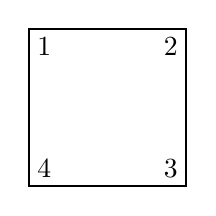
\begin{tikzpicture}
		\node[draw=black, thick,minimum width=2cm,minimum height=2cm] (rect) at (0,0) {};
		\foreach \anc/\n in {south west/4,north west/1,north east/2,south east/3}{
			\node[anchor=\anc] at (rect.\anc) {\n};
		}
	\end{tikzpicture}
	\end{equation*}
	Now, there are four rotations of this square about its center, resulting in the permutations (falling to the shorter notation) $(1\;2\;3\;4), (2\;3\;4\;1), (3\;4\;1\;2), (4\;1\;2\;3)$. There are two reflections about a line passing through the center and one of the vertices (as if the line passes through one vertex, it also passes by the one directly across the center), those result in the permutations $(1\;4\;3\;2)$ and $(3\;2\;1\;4)$. There are also the two reflections about a line passing through the center and a middle of one of the sides, there we get $(2\;1\;4\;3)$ and $(4\;3\;2\;1)$. But that is all the $8$ symmetries of this square, thus we have a homomorphism $D_8 \to S_4$.
\end{proof}

% Problem 2.5
\begin{problem}
\end{problem}

\begin{solution}
	Let $D_{2n}$ be a dihedral group, i.e. the group of symmetries of a regular polygon with $n$ vertices. Let $x$ be a reflection about the center of the polygon and any vertex. Clearly, it must hold that $x^2 = e$, as reflecting about the same line twice returns all the vertices to their original places. Let $y$ be a counterclockwise rotation by $2\pi/n$. Rotating the polygon $n$ times gives us back the original polygon, and thus $y^n=e$.  Now, notice that composing those two symmetries like $xyxy$ gives us back the original polygon, thus $(xy)^2=e$. Manipulating this equation we get $yx=xy^{-1}=xy^{n-1}$ (as $y^{-1}=y^{n-1}$). 
	
	Using these relations we can simplify any product in $D_{2n}$. Suppose $x^{i_1}y^{j_1}x^{i_2}y^{j_2}\dots$ is such a product and without loss of generality suppose $i_k < 2$ and $j_k < n$ for $k \in \mathbb{N}$ (due to the $x^2=e$ and $y^n=e$ relations). Now, we can use the relation $yx = xy^{n-1}$ to move all the $x$ in the product to the right. Thus we can in fact simplify any product in $D_{2n}$ to $x^i y^j$ for $0 \leq i < 2, 0 \leq j < n$.
\end{solution}

% Problem 2.6
\begin{problem}
\end{problem}

\begin{solution}
	For the case $n=1$, we can easily take $g=h$, since $\abs{g}=2$, we have $gg=e$ and thus $\abs{gh}=1$ as needed.
	
	Now suppose $n > 1$. Now consider the group $D_{2n}$. By Problem II.2.5. there are elements $x,y \in D_{2n}$ such that $\abs{x}=2$, $\abs{y}=n$ and $\abs{xy}=2$. Let us define $g = xy$ and $h = x$ (so that $\abs(g)=\abs(h)=2$). We have $gh = xyx = y^{-1}$ and thus $\abs{gh}=\abs{y^{-1}}=\abs{y}=n$.
\end{solution}

% Problem 2.7
\begin{problem}
\end{problem}

\begin{solution}
	By Problem II.2.6. any element of $D_{2n}$ can be written as a product $xy^i$ or $y^i$, $0 \leq i < n$. Now, consider the elements of the form $y^i$, $0 < i < n$. For $y^i$ to commute with $x$, we need to have $x y^i=y^i x$ by definition. But $x y^i = x y y^{i-1} = y^{-i} x$ (as $\abs{xy}=2$). But that means $y^i = y^{-i}=(y^i)^{-1}$ and thus $\abs{y^i}=2$. But by Proposition I.1.13. we know that $\abs{y^i}=\frac{\abs{y}}{\gcd(i, \abs{y}}=\frac{n}{\gcd(i,n)}=2$. So in particular $\gcd(i,n)=\frac{n}{2}$. Since $i < n$, it follows that $i=\frac{n}{2}$.
		
	Now consider elements of the form $xy^i$. If such an element commutes with everything, it has to commute with $x$ in particular. We have $xxy^i=y^i$ and $xy^ix=x^2y^{-i}=y^{-i}$. Now this can only happen for $i = \frac{n}{2}$. Now, it must also commute with $y$. We have $yxy^i=xy^{i-1}$ and $xy^{i}y=xy^{i+1}$. Now, $xy^{i-1}=xy^{i+1}$ would mean $y^{i-1}=y^{i+1}$, which in turn would mean $y^2=e$. But that only happens if $n=2$.
	
	Therefore we have found that there are no elements that commute with everything for groups $D_{2n}$ where $n$ is odd. In the case $n=2$, $y$ and $xy$ commute with everything. In the case $n > 2$, the only such element is $y^{\frac{n}{2}}$, which of course only exists if $n$ is even.
\end{solution}

% Problem 2.8
\begin{problem}
\end{problem}

\begin{solution}
	[not interested]
\end{solution}

% Problem 2.9
\begin{problem}
\end{problem}

\begin{solution}
	Let $n\in\mathbb{N}$ and $\equiv$ be the 'congruence modulo $n$' relation. Now, let $a,b,c \in \mathbb{Z}$ be numbers. We will prove that $\equiv$ is an equivalence relation:
	\begin{itemize}
		\item We have $a-a=0$ and trivially $n | 0$, thus $a \equiv a$.
		\item Suppose $a \equiv b$. Then $n | (b - a)$ by definition. But then there is $k \in \mathbb{Z}$ such that $(b - a) = kn$. But then $-(b - a) = (a - b) = -kn$, and that means $n | (a - b)$. Therefore $b \equiv a$.
		\item Suppose $a \equiv b$ and $b \equiv c$. Then we have $n | (b - a)$ and $n | (c - b)$. But then there are $k,l \in \mathbb{Z}$ such that $(b - a) = kn$ and $(c - b) = ln$. Summing those two equations we obtain $(b - a) + (c - b) = (c - a) = kn + ln = (k + l)n$ and thus $a \equiv c$.
	\end{itemize}
\end{solution}

% Problem 2.10
\begin{problem}
\end{problem}

\begin{solution}
	Let $\mathbb{Z}/n\mathbb{Z}$ be a cyclic group. The group is the set of equivalence classes of congruence modulo $n$ on $\mathbb{Z}$. Clearly, the $n$ elements $[0]_n,[1]_n,\dots,[n-1]_n$ are all distinct, as if we had $[i]_n = [j]_n$, $0 \leq i < j < n$ (clearly it does not matter if $i < j$ or $j < i$), then $i \equiv j$ so $n | (j - i)$ and thus $j - i = kn$ for some $k \in \mathbb{Z}$. But that is a contradiction, as $i < j < n$ so $j - i < n$ and $i \neq j$ so $j - i \neq 0$.
	
	Now, let $m \in \mathbb{Z}$ be a number such that $m < 0$ or $n \leq m$. Then we can divide $m$ by $n$ such that we get $n = km + i$ for some $k \in \mathbb{Z}$ and $0 \leq i < n$. But that means $n | (m - i)$ and thus $m \equiv i$ and therefore $[m]_n = [i]_n$.
	
	Thus, there are precisely $n$ elements of $\mathbb{Z}/n\mathbb{Z}$ given above.
\end{solution}

% Problem 2.11
\begin{problem}
\end{problem}

\begin{solution}
	Let $n \in \mathbb{Z}$ be an odd integer. Then we can write $n=2k+1$ for some $k \in \mathbb{Z}$ by the definition of an odd integer. Then we have $n^2=(2k+1)^2=4k^2+4k+1$. Now, there are two possibilities, either $k$ is even, or $k$ is odd.
	
	Suppose $k$ is even, then $k = 2l$ for some $l \in \mathbb{Z}$. But then $n^2=16l^2+8l+1$, which means $8 | n^2-1$, so that $n \equiv 1 \mod 8$.
	
	Now suppose $k$ is odd, then $k=2l+1$ for some $l \in \mathbb{Z}$. Then $n^2=16l^2+16l+4+8l+4+1=16l^2+24l+9$ so that again $8 | n^2 - 1$ and thus $n \equiv 1 \mod 8$.
\end{solution}

% Problem 2.12
\begin{problem}
\end{problem}

\begin{solution}
	If there are some nonzero integers $a, b, c \in \mathbb{Z}$ such that $a^2+b^2=3c^2$, then the equation $[a]^2_4+[b]^2_4=3[c]^2_4$ in $\mathbb{Z}/4\mathbb{Z}$ would also have to hold. Now, notice that for any $n \in \mathbb{Z}$, $[n]^2_4$ can either equal $0$ (if $n$ is even) or $1$ ($n$ odd). Therefore for the equation to hold in $\mathbb{Z}/4\mathbb{Z}$, $a, b, c$ all have to be even. Let $a=2k, b=2l, c=2m$ for some $k,l,m \in \mathbb{Z}$. Then we have $k^2+l^2=3m^2$. But again, $k,l,m$ have to be even. We can continue this process until we reach $1$ for some of the factors, proving that indeed $a^2+b^2=3c^2$ does not have a non trivial solution in $\mathbb{Z}$.
\end{solution}

% Problem 2.13
\begin{problem}
\end{problem}

\begin{solution}
	Suppose that $m,n \in \mathbb{Z}$ are numbers such that $\gcd(m,n) = 1$. Then by Corollary II.2.5. we see that $[m]_n$ is a generator of $\mathbb{Z}/n\mathbb{Z}$. But there is some $a \in \mathbb{Z}$ such that $a[m]_n=[am]_n=[1]_n$. But that means $am \equiv 1 \mod n$, so $n | (am - 1)$, and therefore $(am - 1) = cn$. But that shows exactly what we required, there are $a,b \in \mathbb{Z}$ such that $am - cn = am + bn = 1$.
	
	Conversely, suppose there are integers $a, b$ such that $am+bn=1$. But then $[am+bn]_n=[am]_n=[1]_n$. But then if $[x]_n \in \mathbb{Z}/n\mathbb{Z}$ is any element of the group, we have $[x]_n=x[1]_n=x[am]_n=xa[m]_n$. But that means $[m]_n$ generates the group, and thus by Corollary II.2.5. $\gcd(m,n)=1$ must hold.
\end{solution}

% Problem 2.14
\begin{problem}
\end{problem}

\begin{solution}
	Suppose $a \equiv a' \mod n$ and $b \equiv b' \mod n$. Then we have $n | (a' - a)$ and thus $a' - a = kn$, similarly we have $b' - b = ln$, for some $k,l \in \mathbb{Z}$. Now, $a'b'-ab=a'b'-(a'-kn)(b'-ln)=a'b'-(a'b'-a'ln-b'kn+lkn^2)=(-a'l-b'k+lkn)n$. But then $n | (a'b'-ab)$, so $[ab]_n=[a'b']_n$. But that means that multiplication of equivalence classes is well-defined.
\end{solution}

% Problem 2.15
\begin{problem}
\end{problem}

\begin{solution}
	Let $n > 0$ be an odd integer.
	\begin{itemize}
		\item Let $m$ be an integer and $\gcd(m,n)=1$. By Exercise II.2.13. there are integers $a,b$ such that $am+bn=1$. We then have $4am+4bn=4am+2n+4bn-2n=2a(2m+n)+(2b-a)2n=4$. That means $\gcd(2m+n,2n) | 4$, as the $\gcd$ must divide the whole equation. But $2m+n$ is odd, since $n$ is odd. Thus $\gcd(2m+n,2n)=1$.
		\item Now, let $r$ be an integer and suppose $\gcd(r,2n)=1$. Then we have, again by Exercise II.2.13., $ar+b2n=1$ for some integers $a,b$. But then we have $ar-an+b2n+an=a(r-n)+(2b+a)n=2a\frac{r-n}{2}=(2b-a)n=1$. Using the result of Exercise II.2.13. again we get $\gcd(\frac{r-n}{2},n)=1$.
		\item Consider the function $f: (\mathbb{Z}/n\mathbb{Z})^* \to (\mathbb{Z}/2n\mathbb{Z})^*$ defined as $f([m]_n)=[2m+n]_{2n}$. Now, this function is well defined, as if $[m]_n \in (\mathbb{Z}/n\mathbb{Z})^*$ we have $\gcd(m,n)=1$ so $\gcd(2m+n,2n)=1$ and thus $[2m+n]_{2n} \in (\mathbb{Z}/2n\mathbb{Z})^*$. Now, define a function $g: (\mathbb{Z}/2n\mathbb{Z})^* \to (\mathbb{Z}/n\mathbb{Z})^*$ as $g([r]_{2n})=[\frac{r-n}{2}]_n$. This function is again well defined. Now, $gf([m]_n)=g([2m+n]_{2n})=[\frac{2m}{2}]_n=[m]_n$ and thus $g$ is a left-inverse of $f$. $fg([r]_{2n})=f([\frac{r-n}{2}]_n)=[2\frac{r-n}{2} + n]_{2n}=[r-n+n]_{2n}=[r]_{2n}$ and thus $g$ is also a right-inverse of $f$. Therefore $f$ is a bijective function. But that means $(\mathbb{Z}/n\mathbb{Z})^*$ and $(\mathbb{Z}/2n\mathbb{Z})^*$ are isomorphic. \qedhere
	\end{itemize}
\end{solution}

% Problem 2.16
\begin{problem}
\end{problem}

\begin{solution}
	To find the last digit of $1238237^{18238456}$ we will work in $\mathbb{Z}/10\mathbb{Z}$. We have $[1238237]_{10}=[7]_{10}$. Now $[7^2]_{10}=[9]_{10}$, $[7^3]_{10}=[3]_{10}$, $[7^4]_{10}=[1]_{10}$. But $[18238456]_{4}=0$, and thus the last digit is $1$.	
\end{solution}

% Problem 2.17
\begin{problem}
\end{problem}

\begin{solution}
	Suppose $m \equiv m' \mod n$. Then $n | (m' - m)$ so $m' - m = kn$ for some integer $k$. Now, suppose that $\gcd(m,n)=1$. Then by Exercise II.2.13. there are integers $a,b$ such that $am+bn=1$. But $m = m' - kn$, so we have $a(m' - kn)+bn=am'-akn+bn=am'+(b-ak)n=1$, and thus $\gcd(m',n)=1$. 
	
	If $\gcd(m',n)=1$, then again there are integers $a,b$ such that $am'+bn=1$. But $m' = kn - m$, so $am'+bn=a(kn - m) + bn=akn-am+bn=(-a)m+(ak+b)n=1$ and thus $\gcd(m,n)=1$.
\end{solution}

% Problem 2.18
\begin{problem}
\end{problem}

\begin{solution}
	Define the function as follows. For $[m]_d$ we move every element up to $d$ $m$ places to the right, wrapping around. This way, $[0]_d$ is the identity permutation, $[1]_d$ is the permutation $(d\;1\;2\;\dots\;d-2\;d-1\;d+1\;\dots n)$. Composing this morphism gets us the permutation $(d-1\;d\;1\dots)$ etc. So indeed, those morphisms preserve the structure.
\end{solution}

% Problem 2.19
\begin{problem}
\end{problem}

\begin{solution}
	Multiplication table for $(\Z{5})^*$:
	
	\begin{center}
		\renewcommand{\arraystretch}{1.3}
		\begin{tabular}{c||c|c|c|c}
			$\cdot$ & $[1]$ & $[2]$ & $[3]$ & $[4]$ \\
			\hline\hline
			$[1]$ & $[1]$ & $[2]$ & $[3]$ & $[4]$ \\ 
			\hline
			$[2]$ & $[2]$ & $[4]$ & $[1]$ & $[3]$ \\ 
			\hline
			$[3]$ & $[3]$ & $[1]$ & $[4]$ & $[2]$ \\ 
			\hline
			$[4]$ & $[4]$ & $[3]$ & $[2]$ & $[1]$ \\ 
		\end{tabular}
	\end{center}

	Multiplication table for $(\Z{12})^*$:
	
	\begin{center}
		\renewcommand{\arraystretch}{1.3}
		\begin{tabular}{c||c|c|c|c}
			$\cdot$ & $[1]$ & $[5]$ & $[7]$ & $[11]$ \\
			\hline\hline
			$[1]$ & $[1]$ & $[5]$ & $[7]$ & $[11]$ \\ 
			\hline
			$[5]$ & $[5]$ & $[1]$ & $[11]$ & $[7]$ \\ 
			\hline
			$[7]$ & $[7]$ & $[11]$ & $[1]$ & $[5]$ \\ 
			\hline
			$[11]$ & $[11]$ & $[7]$ & $[5]$ & $[1]$ \\ 
		\end{tabular}
	\end{center}

	Now note that we can clearly see $(\Z{12})^*$ has $3$ elements of order $2$, but $(\Z{5})^*$ has two elements of order $4$ and a single element of order $2$. Therefore we cannot relabel the elements in a way the two groups would correspond.
\end{solution}

x\subsection{The category $\mathsf{Grp}$}

% Problem 3.1
\begin{problem}
\end{problem}

\begin{solution}
	Let $\C$ be a category with products and $\varphi: G \to H$ a morphism in $\C$. Now, if we have products $G \times G$ and $H \times H$ with the morphisms $\pi_G,\pi'_G: G \times G \to G$ and $\pi_H,\pi'_H: H \times H \to H$, we can use the universal property of products as follows: Since $H \times H$ with $\pi_H,\pi'_H$ satisfies the universal property, for any object $X$, such that there are morphisms $f_H,f'_H: X \to H$, there is a unique morphism $X \to H \times H$. Now notice that for $G \times G$ we have two morphisms $\varphi \circ \pi_G: G \times G \to H$ and $\varphi \circ \pi'_G: G \times G \to H$. Therefore due to the unique property of products there is a unique morphism $\varphi \times \varphi: G \times G \to H \times H$ such that $\pi_H \circ (\varphi \times \varphi) = \varphi \circ \pi_G$ and $\pi'_H \circ (\varphi \times \varphi) = \varphi \circ \pi'_G$.
\end{solution}

% Problem 3.2
\begin{problem}
\end{problem}

\begin{solution}
	Let $\C$ be a category with products and $\varphi: G \to H$ and $\psi: H \to K$ morphisms in $\C$. By Exercise II.3.1. there are then morphisms $(\varphi \times \varphi): G \times G \to H \times H$ and $(\psi \times \psi): H \times H \to K \times K$ and also $(\psi \circ \varphi) \times (\psi \circ \varphi): G \times G \to K \times K$ (since $\psi \circ \varphi: G \to K$) compatible with the natural projections. Now we will prove the diagram
	
	\begin{equation*}
		\begin{tikzcd}[column sep=huge]
			& & K \\
			G \times G
			\arrow[r, "(\psi \times \psi) \circ (\varphi \times \varphi)"]
			\arrow[urr, bend left=20, "\psi \circ \varphi \circ \pi_G"]
			\arrow[drr, bend right=20, "\psi \circ \varphi \circ \pi'_G"'] &
			K \times K
			\arrow[ur, "\pi_K"]
			\arrow[dr, "\pi'_K"'] & \\
			& & K \\
		\end{tikzcd}
	\end{equation*}
	
	commutes. Note that by Exercise II.3.1. we have $\pi_K \circ (\psi \times \psi) = \psi \circ \pi_H$ and $\pi_H \circ (\varphi \times \varphi) = \varphi \circ \pi_G$. Thus we have
	
	\begin{equation*}
		\begin{aligned}
			\pi_K \circ (\psi \times \psi) \circ (\varphi \times \varphi) &={} \psi \circ \pi_H \circ (\varphi \times \varphi)\\ &={} \psi \circ \varphi \circ \pi_G
		\end{aligned}
	\end{equation*}
	
	 and similarly for the other side. But we know $(\psi \circ \varphi) \times (\psi \circ \varphi)$ is the unique morphism making the diagram commute (by Exercise II.3.1.) and therefore $(\psi \circ \varphi) \times (\psi \circ \varphi) = (\psi \times \psi) \circ (\varphi \times \varphi)$.
\end{solution}

% Problem 3.3
\begin{problem}
\end{problem}

\begin{solution}
		Suppose $G$ and $H$ are abelian groups. Consider the product of those groups, $G \times H$, with the two natural homomorphisms $i_G: G \to G \times H$ ($g \mapsto (g, e_H)$) and $i_H: H \to G \times H$ ($h \mapsto (e_G, h)$). For this construction to satisfy the universal property of coproducts in $\mathsf{Ab}$, for any abelian group $Z$ such that there are homomorphisms $f_G: G \to Z$ and $f_H: H \to Z$, there must be a unique homomorphism $\sigma: G \times H \to Z$ making
		\begin{equation*}
			\begin{tikzcd}
				G
					\arrow[drr, bend left=20, "f_G"]
					\arrow[dr, "i_G" swap]
					& &\\
				&
					G \times H
						\arrow[r, "\sigma"]
					& Z\\
				H
					\arrow[urr, bend right=20, "f_H"']
					\arrow[ur, "i_H"]
					& &
			\end{tikzcd}
		\end{equation*}
		commute. Now, the only choice for $\sigma$ is given by the set-function $\sigma((a,b))=f_G(a)f_H(b)$. We have to check that $\sigma$ is a group homomorphism.
		We have
		\begin{equation*}
			\begin{aligned}
				\sigma((a,b)(c,d)) &= \sigma((ac,bd))\\
				&= f_G(ac)f_H(bd)\\
				&= f_G(a)f_G(c)f_H(b)f_H(d)\\
				&= f_G(a)f_H(b)f_G(c)f_H(d)\\
				&=\sigma((a,b))\sigma((c,d))
			\end{aligned}
		\end{equation*} 
		precisely because $Z$ is commutative. Therefore, $G \times H$ satisfies the universal propery of coproducts in $\C$.
\end{solution}

% Problem 3.4
\begin{problem}
\end{problem}

\begin{solution}
	$H$ does not necessarily have to be the trivial group. We can consider a countably infinite product $G = H \times H \dots$. Then indeed $G \cong G \times H$.
\end{solution}

% Problem 3.5
\begin{problem}
\end{problem}

\begin{solution}
	Let $\mathbb{Q}=G \times H$. If both $G, H$ are trivial, then $\mathbb{Q}$ would be trivial, and thus, without loss of generality, say that $G$ is non-trivial. Now, consider the canonical projection $\pi_G$.
	
	We will show that $\pi_G$ is in fact an injective homomorphism. First of all, notice that for $m \neq 0$ and any $g \in G$ such that $g^m = e_G$ we have $(g, e_H)^m = (g^m, e_H) = (e_G, e_H)$. But $\mathbb{Q}$ has no non-zero elements of finite order, and thus $g = e_G$.
	
	Now suppose that $\pi_G$ is not an injective homomorphism and thus there are two rational numbers $\frac{a_1}{b_1}, \frac{a_2}{b_2}$, such that $a_1, a_2, b_1, b_2 \neq 0 \in \mathbb{Z}$ and $\frac{a_1}{b_1} \neq \frac{a_2}{b_2}$, for which $\pi_G(\frac{a_1}{b_1}) = \pi_G(\frac{a_2}{b_2})$. Then we have $\pi_G(\frac{a_1}{b_1})^{b_1 b_2} = \pi_G(a_1)^{b_2} = \pi_G(1)^{a_1 b_2}$ and similarly $\pi_G(\frac{a_2}{b_2}) = \pi_G(1)^{a_2 b_1}$ (because $\pi_G$ is a group homomorphism). Then we must have $\pi_G(1)^{a_1 b_2} = \pi_G(1)^{a_2 b_1}$ and thus $\pi_G(1)^{a_1 b_2 - a_2 b_1} = e_G$. But that means $\pi_G(1) = e_G$ (by the last paragraph) and thus $\pi_G$ maps every integer to $e_G$.
	
	Now suppose $\frac{a}{b}$ is a rational number, $a, b \neq 0 \in \mathbb{Z}$. Now $\pi_G(\frac{a}{b})^b = \pi_G(a) = e_G$. But by the same argument of order we thus have $\pi_G(\frac{a}{b}) = e_G$. That means $\pi_G$ maps everything to $e_G$. Since $\pi_G$ is necessarily a surjective homomorphism, $G$ is trivial, a contradiction. Therefore $\pi_G$ must be an injective homomorphism. But since $\pi_G((e_G,h))=e_G$ for all $h \in H$ by definition, $H$ must necessarily be trivial.
\end{solution}

% Problem 3.6
\begin{problem}
\end{problem}

\begin{solution}
	Going point by point:
	\begin{itemize}
		\item Let $f: C_2 \to S_3$ be defined as $f(e) = (1\;2\;3)$ and $f(x) = (2\;1\;3)$. Then $f(x^n)=e$ if $2 | n$ or $f(x^n)=(2\;1\;3)$ otherwise. Thus this is an injective homomorphism. Now, let $g: C_3 \to S_3$ be defined as $g(e)=(1\;2\;3)$, $g(x)=(2\;3\;1)$ and $g(x^2)=(3\;1\;2)$. Now, $g(x)g(x)=(3\;1\;2)=g(x^2)$, and $g(x)g(x^2)=(1\;2\;3)$, so it is indeed an injective homomorphism.
		\item Suppose $C_2 \times C_3$ is the coproduct of $C_2$ and $C_3$ in $\mathsf{Grp}$. By the universal property of coproducts,  as there are morphisms $C_2 \to S_3$ and $C_3 \to S_3$, this means there is a unique homomorphism $\sigma: C_2 \times C_3 \to S_3$, such that $\sigma i_{C_2} = f$ and $\sigma i_{C_3} = g$.
		\item Now, notice that $i_{C_2}$ must necessarily map an element $x \in C_2$ to $(x, e_{C_3})$, and similarly for $i_{C_3}$. But then we have $f(x_1)g(x_2)=\sigma((x_1, e_{C_3})(e_{C_2}, x_2))=\sigma((x_1, x_2))=\sigma((e_{C_2}, x_2)(x_1, e_{C_3})=g(x_2)f(x_1)$. But we have, for example, $(2\;1\;3)(2\;3\;1)=(3\;2\;1)$ and $(2\;3\;1)(2\;1\;3)=(1\;3\;2)$. Thus $\sigma$ cannot exist (precisely because $S_3$ is not commutative). \qedhere
	\end{itemize}
\end{solution}

% Problem 3.7
\begin{problem}
\end{problem}

\begin{solution}
	Let $\mathbb{Z} \ast \mathbb{Z}$, $C_2 \ast C_3$ be a coproduct in $\Cgrp$. Let $A$ be a group and $\alpha': C_2 \ast C_3 \to $ and $\alpha'': C_2 \ast C_3 \to A$ any two homomorphisms. Consider the diagram
	
	\begin{equation*}
		\begin{tikzcd}
			\mathbb{Z} 
			\arrow[rr]
			\arrow[dr, "i_\mathbb{Z}"] & & 
			C_2
			\arrow[dr, "i_{C_2}"]
			\arrow[drr, bend left=20, "\alpha' i_{C_2}"] & & \\
			& \mathbb{Z} \ast \mathbb{Z}
			\arrow[rr, dashrightarrow, "\sigma"] & & 
			C_2 \ast C_3 
			\arrow[r, shift left, "\alpha'"]
			\arrow[r, shift right, "\alpha''"'] & A \\
			\mathbb{Z}
			\arrow[rr]
			\arrow[ur, "i'_\mathbb{Z}"'] & & 
			C_3
			\arrow[ur, "i_{C_3}"']
			\arrow[urr, bend right=20, "\alpha'' i_{C_3}"'] & & \\
		\end{tikzcd}
	\end{equation*}
	
	Now, by the universal property of coproducts, $\sigma$ is a unique homomorphism making the diagram commute. Notice, that by the universal property of coproducts we can also see $\alpha'$ is the unique homomorphism making the right half of the diagram commute. But that means $\alpha' = \alpha''$ and thus $\sigma$ is an epimorphism. But that means it is a surjective set-function and thus a surjective homomorphism.
\end{solution}

% Problem 3.8
\begin{problem}
\end{problem}

\begin{solution}
	Define a group $G$ as the group generated by two elements $x, y$ such that $x^2=e_G$ and $y^3=e_G$. Then we can define group homomorphisms $i_{C_2}: C_2 \to G$ and $i_{C_3}: C_3 \to G$ as follows: $i_{C_2}(e_{C_2})=e_G$, $i_{C_2}(c_2)=x$, $i_{C_3}(e_{C_3})=e_G$, $i_{C_3}(c_3)=y$, $i_{C_3}(c_3^2)=y^2$.
	
	Suppose $Z$ is any group, and $f: C_2 \to Z$ and $g: C_3 \to Z$ group homomorphisms. To prove that $G$ satisfies the universal property of coproducts in $\mathsf{Grp}$ we have to construct a group homomorphism $\sigma: G \to Z$, such that $\sigma i_{C_2} = f$ and $\sigma i_{C_3} = g$. Now notice that we must have $\sigma i_{C_2} (c_2) = \sigma(x) = f(c_2)$ and $\sigma i_{C_3} = \sigma(y) = g(c_3)$. Since $x$ and $y$ generate every element of $G$, this is enough for us to construct $\sigma$. If $x^{i_0} y^{j_0} x^{i_1} y^{j_1} \dots$ where $0 \leq i_0, i_1, \dots < 2$ and $0 \leq j_0, j_1 \dots < 3$ is an element of $G$, we define $\sigma(x^{i_0} y^{j_0} x^{i_1} y^{j_1} \dots)  = f(c_2)^{i_0} g(c_3)^{j_0} \dots$.
	
	It is clear that $\sigma$ is a homomorphism that makes the relevant diagram commute.
\end{solution}

% Problem 3.9
\begin{problem}
\end{problem}

\begin{solution}
	The definition of the fiber product is pretty straightforward, and follows straight from the definition for $\mathsf{Set}$. We only have to check that the definition indeed results in a group and satisfies the required universal property. Let $A,B,C$ be groups and $\alpha: A \to C$, $\beta: B \to C$ group homomorphisms. Define $A \times_C B = \set{(a,b) \in A \times B \mid \alpha(a)=\beta(b)}$.
	
	To check that this construction is a group, we will take the operation to be the same as the one on $A \times B$, i.e. $(a,b)(c,d)=(ac,bd)$. This operation is well-defined, as we have $\alpha(a)=\beta(b)$ and $\alpha(c)=\beta(d)$, and since $\alpha, \beta$ are group homomorphisms, $\alpha{ab}=\alpha(a)\alpha{b}=\beta{c}\beta{d}=\beta{cd}$. Now, we have to prove that $(e_A, e_B)$ is an element of the group. But we have $\alpha(e_A)=e_C=\beta(e_B)$, again because they are homomorphisms. Now, suppose $(a,b) \in A \times_C B$. Then $\alpha(a)=\beta(b)$, so $(\alpha(a))^{-1}=(\beta(b))^{-1})$ and again because they are homomorphisms, $\alpha(a^{-1})=\beta(b^{-1})$. Therefore $(a^{-1}, b^{-1}) \in A \times_C B$, but that is an inverse of $(a, b)$. Thus $A \times_C B$ is a group.
	
	Now, we have to prove that this construction satisfies the universal property of a fiber product. Suppose $Z$ is a group and $f, g$ the respective homomorphisms, such that $\alpha f = \beta g$. To ensure the commutativity of the respective diagram, we have to define $\sigma: Z \to A \times_C B$ as follows: $\sigma(z)=(f(z),g(z))$.  It is well defined, as we have $(\alpha f)(z) = (\beta g)(z)$, so $\alpha (f(z))=\beta(g(z))$. To see that this is a group homomorphism, note that $\sigma(z_1 z_2) = (f(z_1z_2), g(z_1z_2)) = (f(z_1)f(z_2),g(z_1)g(z_2))=(f(z_1), g(z_1))(f(z_2), g(z_2))=\sigma(z_1)\sigma(z_2)$.

	The commutativity of the diagram follows from the definition easily, note that we have $(\pi_A \sigma)(z)=\pi_A(\sigma(z))=\pi_A((f(z), g(z)))=f(z)$ so $\alpha \pi_A \sigma = \alpha f$ and similarly for the other side of the diagram.
	
	To define the fibered coproduct in $\mathsf{Ab}$ we require knowledge of quotients, which have yet to be introduced.
\end{solution}

\subsection{Group homomorphisms}

% Problem 4.1
\begin{problem}
\end{problem}

\begin{solution}
	Suppose $m | n$ and $a \equiv a' \mod n$. Then $n | (a' - a)$. But then $m | (a' - a)$, and thus $[a]_m = [a']_m$.
	
	To check it makes the diagram commute, notice that for any $z \in \mathbb{Z}$ we have $(\pi^n_m \pi_n)(z)=\pi^n_m([z]_n)=[z]_m=\pi_m(z)$ by the definition of the function.
	
	To verify it is indeed a group homomorphism, let $a,b$ be elements of $\mathbb{Z}_n$. Then we have $\pi^n_m(a+b)=[a+b]_m=[a]_m + [b]_m = \pi^n_m(a) + \pi^n_m(b)$.
	
	Thus $\pi^n_m$ is a well-defined group homomorphism that makes the diagram commute. The hypothesis $m | n$ is necessary as the order of all elements of $\mathbb{Z}_n$ divides $n$ and the order of all elements of $\mathbb{Z}_m$ divides $m$, and it also must hold that $\abs{\pi^n_m(z)} \mid \abs{z} \mid n$. Now if $m \nmid n$, then $\pi^n_m([1]_n)=[1]_m$ but $\abs{\pi^n_m([1]_n)}=m \nmid n$, a contradiction.
\end{solution}

% Problem 4.2
\begin{problem}
\end{problem}

\begin{solution}
	The homomorphism is defined pretty explicitly so we can easily check that the image of the homomorphism is the set $\set{(0,0),(1,1)}$, which is in fact not isomorphic to the set underlying $C_2 \times C_2$. We can actually show that there is no such isomorphism. 
	
	In fact, there is no isomorphism of the two groups. The generator of $C_4$ has order $4$, but there is no such element in $C_2 \times C_2$ (all non-zero elements have order $2$).
\end{solution}

% Problem 4.3
\begin{problem}
\end{problem}

\begin{solution}
	Suppose $G$ is a group of order $n$ isomorphic to $\mathbb{Z}/n\mathbb{Z}$. Let $\varphi: \Z{n} \to G$ be a group isomorphism. There is an element of order $n$ in $\Z{n}$, namely $[1]_n$. By Proposition II.4.8. $\abs{\varphi([1]_n)}=\abs{[1]_n}=n$, thus $G$ contains an element of order $n$.
	
	Suppose the converse holds, i.e. $G$ is a group of order $n$ which contains an element $x$ of 
	order $n$. Because $x$ has order $n$, the elements $x^0, x^1, \dots, x^{n-1}$ must make up all of G (if some of those elements were equal, it would be a contradiction to the order of $x$ by cancellation). We can define a homomorphism $\varphi: \Z{n} \to G$ as $\varphi([i]_n) = x^i$.
	
	This is a homomorphism as $\varphi([i]_n + [j]_n) = \varphi([i + j]_n) = x^{i + j} = x^i x^j = \varphi([i]_n) \varphi([j]_n)$.
	
	Now define $\rho: G \to \Z{n}$ as $\rho(x^i) = [i]_n$. It is easy to see that this is an inverse of $\varphi$ and thus $\varphi$ is an isomorphism of groups.
\end{solution}

% Problem 4.4
\begin{problem}
\end{problem}

\begin{solution}
	\begin{itemize}
		We will consider the groups one by one:
		
		\item Consider $(\mathbb{Z}, +)$. Notice that any element $z \in \mathbb{Z}$ is equal to $z \cdot 1$. Therefore any homomorphism $\varphi: (\mathbb{Z}, +) \to G$ (where $G$ is any group) is uniquely determined by $\varphi(1)$. Let $G = \mathbb{Q}$ (or $\mathbb{R}$) and suppose $\varphi(1) = \frac{a}{b}$ for some $a, b \neq 0 \in \mathbb{Z}$. Then $\varphi(z) = z \varphi(1) = z \frac{a}{b} = \frac{z \cdot a}{b}$. But that clearly means there is no number $z$ such that $\varphi(z) = \frac{a}{b+1}$. Thus $\varphi$ is not surjective and therefore it cannot be an isomorphism.
		
		\item Now consider $(\mathbb{Q}, +)$. Let $x, y \in \mathbb{Q}$, clearly, we can always find non-zero integers $a, b$ such that $a x = b y$. However, this is not true in $\mathbb{R}$, if for example $x = \sqrt{2}$ and $y = 1$. Thus the two groups cannot be isomorphic.
		
		\item $(\mathbb{R}, +)$ and $(\mathbb{C}, +)$ are in fact isomorphic. However the construction of the isomorphism is fairly involved. \qedhere
	\end{itemize}
\end{solution}

% Problem 4.5
\begin{problem}
\end{problem}

\begin{solution}
	Notice that $i$ has order $4$ in $(\mathbb{C} \setminus 0, \cdot)$. However, there is no element of $(\mathbb{R} \setminus 0, \cdot)$ of order $4$. Since isomorphism preserves order of elements, it follows that the two groups are not isomorphic.
\end{solution}

% Problem 4.6
\begin{problem}
\end{problem}

\begin{solution}
	The two groups are not isomorphic. Suppose there is an isomorphism $\varphi: (\mathbb{Q}, +) \to (\mathbb{Q}^{>0}, \cdot)$. Let $y$ be a number such that $\varphi(y) = 2$ (there must be such a number because $\varphi$ is an isomorphism). Now we can find a number $x \in \mathbb{Q}$ such that $x + x = y$ in $(\mathbb{Q}, +)$. But then $\varphi(y) = \varphi(x + x) = \varphi(x) \varphi(x) = \varphi^2(x) = 2$. But we know there is no number in $\mathbb{Q}$ with this property.
\end{solution}

% Problem 4.7
\begin{problem}
\end{problem}

\begin{solution}
	Let $G$ be a group and $g, h$ be elements $G$. 
	
	Consider the function $\varphi: G \to G$, $\varphi(g) = g^{-1}$. Suppose $\varphi$ is a group homomorphism. Then we have $hg = (g^{-1} h^{-1})^{-1} = \varphi(g^{-1} h^{-1}) = \varphi(g^{-1})\varphi(h^{-1}) = gh$. But that means precisely that $G$ is an abelian group. Now suppose $G$ is abelian. Then $\varphi(gh) = (gh)^{-1} = h^{-1} g^{-1} = \varphi(h) \varphi(g) = \varphi(g) \varphi(h)$. And thus $\varphi$ is a group homomorphism.
	
	Consider the function $\psi: G \to G$, $\psi(g) = g^2$. Suppose $\psi$ is a group homomorphism. Then $ghgh = (gh)^2 = \psi(gh) = \psi(g) \psi(h) = g^2 h^2 = gghh$. By cancellation we then have $hg = gh$ and thus $G$ is abelian. Now suppose $G$ is abelian. Then $\psi(gh) = (gh)^2 = ghgh = gghh = g^2 h^2 = \psi(g) \psi(h)$. And thus $\psi$ is a group homomorphism.
\end{solution}

% Problem 4.8
\begin{problem}
\end{problem}

\begin{solution}
	Let $G$ be a group, and let $g \in G$. Consider the function $\gamma_g: G \to G$, $\gamma_g(a) = gag^{-1}$. Let $a, b \in G$. Then $\gamma_g(ab) = g(ab)g^{-1} = gag^{-1}gbg^{-1} = \gamma_g(a) \gamma_g(b)$. Thus $\gamma_g$ is a group homomorphism. Now let $\varphi_g: G \to G$ be a function defined as $\varphi_g(a) = g^{-1}ag$. Clearly this is also a group homomorphism. For $a \in G$ we have $(\gamma_g \circ \varphi_g)(a) = \gamma_g(\varphi_g(a)) = \gamma_g(g^{-1}ag) = gg^{-1}agg^{-1} = a$ and $(\varphi_g \circ \gamma_g)(a) = \varphi_g(\gamma_g(a)) = \varphi_g(gag^{-1}) = g^{-1}gag^{-1}g = a$. Thus $\varphi_g$ is an inverse of $\gamma_g$ and therefore $\gamma_g$ is an automorphism of $G$.
	
	Consider the function $\psi: G \to \Aut(G)$, $\psi(g) = \gamma_g$. Let $g, h \in G$. We have $\psi(gh) = \gamma_{gh}$. Now let $a$ be any element of $G$. We then have $\gamma_{gh}(a) = (gh)a(gh)^{-1} = ghah^{-1}g^{-1} = g \gamma_h(a) g^{-1} = \gamma_g(\gamma_h(a)) = \gamma_g \circ \gamma_h$. Thus $\psi(gh) = \gamma_{gh} = \gamma_g \circ \gamma_h = \psi(g) \circ \psi(h)$ and therefore $\psi$ is in fact a group homomorphism.
	
	Now suppose $\psi$ is trivial. Then for any $g \in G$ we have $\psi(g) = \gamma_g = id_G$. But that means for every $a \in G$ we must have $gag^{-1} = a$ and thus $ga = ag$ and therefore $G$ must be abelian. Now suppose $G$ is abelian. For any $a, g \in G$ we then have $\gamma_g(a) = gag^{-1} = gg^{-1}a = e_G a = a$, but that means $\gamma_g = id_G$ for every $g$ and thus $\psi$ is a trivial homomorphism.
\end{solution}

% Problem 4.9
\begin{problem}
\end{problem}

\begin{solution}
	Suppose $m, n$ are positive integers and $\gcd(m, n) = 1$. The order of $[1]_m$ in $\Z{m}$ is $m$ and the order of $[1]_n$ in $\Z{n}$ is $n$. Consider the element $([1]_m, [1]_n)$ of $\Z{m} \times \Z{n}$. Suppose the order of $([1]_m, [1]_n)$ is $x$, so that $x ([1]_m, [1]_n) = ([0]_m, [0]_n)$, which in turn means $x [1]_m = [0]_m$ and $x [1]_n = [0]_n$. Therefore $m \mid x$ and $n \mid x$. Therefore $\lcm(m, n) \mid x$. But $\lcm(m, n) = mn$ as $\gcd(m, n) = 1$. Thus $mn$ must be the order of $([1]_m, [1]_n)$. Now notice that the order of $\Z{m} \times \Z{n}$ is $mn$. Thus by Problem II.4.3. that means $\Z{m} \times \Z{n} \cong \Z{mn}$.
\end{solution}

% Problem 4.10
\begin{problem}
\end{problem}

\begin{solution}
	Let $p \neq q$ be odd prime integers. By definition, $(\Z{pq})^* = \{[n]_{pq} \in \Z{pq} \mid \gcd(n, pq) = 1\}$. By Problem II.4.9., we have $\Z{pq} \cong \Z{p} \times \Z{q}$ as $\gcd(p, q) = 1$. But then we can conclude $(\Z{p})^* \times (\Z{q})^* \cong (\Z{pq})^*$.
	
	Notice, that $[p-1]^2_p = [p^2 - 2p + 1]_p = [1]_p$ and similarly for $[q-1]^2_q = [1]_q$. But then we have two different elements $([p-1]_p, [1]_q)$ and $([1]_p, [q-1]_q)$ in $(\Z{p})^* \times (\Z{q})^*$ of order $2$. Therefore there are two elements $x \neq y \in {\Z{pq}}^*$ of order $2$.
	
	Now, the order of $(\Z{p})^* \times (\Z{q})^*$ is $(p-1)(q-1)$, and therefore even. Suppose $(\Z{pq})^*$ is cyclic and let $g$ be a generator of this group. Then $\abs{g} = (p-1)(q-1)$. Suppose $g^k$ has order $2$, where $0 < k < (p-1)(q-1)$. Then $g^{2k}$ is the identity. Therefore, since the group is cyclic, $(p-1)(q-1) \mid 2k$, which forces $k = \frac{(p-1)(q-1)}{2}$. But that is a contradiction to the fact that $(\Z{pq})^*$ actually contains two different elements of order $2$.
\end{solution}

% Problem 4.11
\begin{problem}
\end{problem}

\begin{solution}
	Let $p$ be a prime integer. Assume that the equation $x^d = 1$ can have at most $d$ solutions in $\Z{p}$.
	
	Let $G = (\Z{p})^*$. $G$ is a commutative group of finite order. Because the order of $G$ is finite, all elements of $G$ also have finite order. Let $g \in G$ be an element of maximal order. Clearly $\abs{g} \leq p-1$. By Problem II.1.15 we can see that for all $h \in G$, $\abs{h}$ divides $\abs{g}$. But that means $h^{\abs{g}} = 1$ for all $h \in G$.
	
	But that means we produced $p-1$ solutions of the equation $x^{\abs{g}} = 1$ in $\Z{p}$ and thus $p-1 \leq \abs{g}$ by the fact we have assumed.
	
	Combining the two inequalities we see that $\abs{g} = p-1$ and thus $G$ is cyclic as it contains an element of order $p-1$.
\end{solution}

% Problem 4.12
\begin{problem}
\end{problem}

\begin{solution}
	\begin{itemize}
		\item The order of $[9]_{31}$ must divide the order of the group, $30$, because it is cyclic. Trying the different divisors we get $[9]^{15}_{31} = [1]_{31}$. Thus $\abs{[9]_{31}} = 15$ in $(\Z{31})^*$.
		\item Consider the equation $x^3 - 9 = 0$ in $\Z{31}$. Suppose that $c$ is a solution of this equation, then we have $c^3 = [9]_{31}$ in $(\Z{31})^*$. Then we must have $\abs{c^3} = \abs{[9]_{31}} = 15$. But $\abs{c^3} = \frac{\lcm(3, \abs{c})}{3}$ by Proposition II.1.13. and thus we have $\frac{\lcm(3, \abs{c})}{3} = 15$ so that $\lcm(3, \abs{c}) = 45$. But then $\abs{c} = 45$ which is a contradiction to the fact $c$ as an element of $(\Z{30})^*$ must have order dividing $30$. Therefore the equation has no solutions. \qedhere
	\end{itemize}
\end{solution}

% Problem 4.13
\begin{problem}
\end{problem}

\begin{solution}
	Consider the group $\Aut_\Cgrp(\Z{2} \times \Z{2})$, the group of isomorphisms of the group $\Z{2} \times \Z{2}$. First we will analyze how the isomorphisms look. Let $1, a, b, c$ label the elements of this group. Suppose $\varphi: \Z{2} \times \Z{2} \to \Z{2} \times \Z{2}$ is a group isomorphism. Then in particular $\varphi$ must be a group homomorphism. Therefore we always have $\varphi(1) = 1$. Clearly we have $3 \cdot 2 = 6$ possible bijections which satisfy this constraint. Now we will show that each such bijection is in fact a group homomorphism. Suppose $\varphi(a) = x, \varphi(b) = y, \varphi(a + b) = \varphi(c) = z$. Because $\varphi$ is a bijection and $a \neq b \neq c$ we have $x \neq y \neq z$ and thus $x + y = z$ and therefore $\varphi(a + b) = \varphi(a) + \varphi(c)$.
	
	But notice that the argument shows that in fact every such $\varphi$ is a permutation of the three elements $a, b, c$. And thus $\Aut_\Cgrp(\Z{2} \times \Z{2}) \cong S_3$
\end{solution}

% Problem 4.14
\begin{problem}
\end{problem}

\begin{solution}
	Consider the group $\Aut_\Cgrp(C_n)$ for some $n$. Now, $C_n$ has a generator $x$ of order $n$. We know that a class $[m]_n$ generates the group $\Z{n}$ if and only if $\gcd(m, n) = 1$ (by Corollary II.2.5.). But every isomorphism $C_n \to C_n$ must send the generator $x$ to one such element relatively prime to $n$, as isomorphisms must keep the order of elements. That means that every such isomorphism is determined by the choice of the image of $x$. Thus the order of $\Aut_\Cgrp(C_n)$ is in fact the number of positive integers $r \leq n$ that are relatively prime to $n$ as required.
\end{solution}

% Problem 4.15
\begin{problem}
\end{problem}

\begin{solution}
	Lets first consider the group of automorphisms of $(\mathbb{Z}, +)$. Clearly we have $z = z \cdot 1$ for every $z \in \mathbb{Z}$ and thus every homomorphism $\varphi$ of $(\mathbb{Z}, +)$ is determined by $\varphi(1)$. Now for $\varphi$ to be a bijection, notice that there are only two possible choices: $\varphi(1) = 1$ (the identity morphism) and $\varphi(1) = -1$. Any other choice leads to $1$ being absent from the image of $\varphi$ and thus $\varphi$ would necessarily not be a bijection. But that means $\Aut_\Cgrp((\mathbb{Z}, +)) \cong C_2$.
	
	Let $p$ be a prime integer. We know $C_p$ has a generator $x$ such that $x^p = 1$. Every isomorphism of $C_p$ is determined by where it maps this generator $x$, an element $x^n$ such that the order of $x^n$ is also $p$ (so that $x^n$ is also a generator of $C_p$). But notice that due to this we can look on $\Aut_\Cgrp(C_p)$ as on $(\Z{p})^*$. But by Problem II.4.14. we know $(\Z{p})^* \cong C_{p-1}$.
\end{solution}

% Problem 4.16
\begin{problem}
\end{problem}

\begin{solution}
	Let $p > 1$ be an integer. Suppose $p$ is prime. Then by Problem II.4.11. we can see $(\Z{p})^*$ is a cyclic group of order $p-1$. Since the group is cyclic, there is exactly one element of order $2$, $[-1]_p$. But then by Problem II.1.8. we know $\prod_{g \in (\Z{p})^*} g = [-1]_p$. But since $p$ is prime, $\prod_{g \in (\Z{p})^*} g = [p-1]_p [p-2]_p \dots [1]_p = [(p-1)!]_p = [-1]_p$. But then $(p-1)! \equiv -1 \mod p$.
	
	Now suppose $(p-1)! \equiv -1 \mod p$ and suppose $d$ is a proper divisor of $p$. Notice that all the proper divisors of $p$ are contained in the product $(p-1)!$ and thus $d$ divides this number. Then in particular $(p-1)! \equiv 0 \mod d$. But since $d \mid p$, we must have $d \mid p \mid (-1 - (p-1)!)$ and thus $(p-1)! \equiv -1 \mod d$. But that forces $d = 1$ and thus $p$ must be prime.
\end{solution}

% Problem 4.17
\begin{problem}
\end{problem}

\begin{solution}
	For $p=5$, $[2]_5$ is a generator of $(\Z{5})^*$ as its order is $4$.
	
	For $p=7$, $[3]_7$ is a generator of $(\Z{7})^*$.
	
	For $p=11$, $[2]_{11}$ is a generator of $(\Z{11})^*$.
	
	For $p=13$, $[2]_{13}$ is a generator of $(\Z{13})^*$.
\end{solution}

% Problem 4.18
\begin{problem}
\end{problem}

\begin{solution}
	Let $\varphi: G \to H$ be an isomorphism. Assume $G$ is commutative. Let $g, g' \in G$, $h, h' \in H$ be any elements such that $\varphi(g) = h, \varphi(g') = h'$. Then we have $h h' = \varphi(g) \varphi(g') = \varphi(gg') = \varphi(g'g) = \varphi(g') \varphi(g) = h' h$ and thus $H$ is commutative.
	
	Now assume $H$ is commutative. Now since $\varphi$ is an isomorphism, there is an inverse $\varphi^{-1}$. Let $g, g' \in G$, $h, h' \in H$ be any elements such that $\varphi^{-1}(h) = g, \varphi^{-1}(h') = g'$. We have $g g' = \varphi^{-1}(h) \varphi^{-1}(h') = \varphi^{-1}(h h') = \varphi^{-1}(h' h) = \varphi^{-1}(h') \varphi^{-1}(h) = g' g$ and therefore $G$ is commutative.
\end{solution}

\subsection{Free groups}

I found it necessary for my understanding of free groups to prove that if $A$ and $B$ are isomorphic sets, then so must the free groups $F(A)$ ($F^{ab}(A)$) and $F(B)$ ($F^{ab}(B)$) be isomorphic.

\begin{proof}
	Let $A, B$ be sets such that $A \cong B$. Then there is a bijection $\psi: A \to B$. We will show that $F(B)$ together with the set-function $\psi \circ j_B$ satisfies the same universal property as $F(A)$. Let $G$ be any group and $f: A \to G$ a set-function. Consider the diagram
	\begin{equation*}
		\begin{tikzcd}[column sep=large, row sep=large]
			F(B)
			\arrow[r, dashrightarrow, "\varphi"]
			& G \\
			B
			\arrow[u, "j_B"]
			\arrow[ur, "f \circ \psi^{-1}" description]
			\arrow[d, shift left, "\psi^{-1}"]
			& \\
			A
			\arrow[u, shift left, "\psi"]
			\arrow[uur, bend right=20, "f"']
			&
		\end{tikzcd} \text{.}
	\end{equation*}
	
	By the universal property of free product $F(B)$ there is a unique homomorphism $\varphi$ making the upper part of the diagram commute, so that $\varphi \circ j_B = f \circ \psi^{-1}$. But then $\varphi \circ j_b \circ \psi = f$ and thus $F(B)$ satisfies the universal property of free group on $A$ and therefore $F(A) \cong F(B)$ as needed.
	
	The situation for free abelian groups is entirely analogous. In particular, any finite set $A$ is isomorphic to the set $\{ 1, 2, \cdots, \abs{A} \}$ and thus $F^{ab}(A) = \Zs^{\oplus \abs{A}}$.
\end{proof}

% Problem 5.1
\begin{problem}
\end{problem}

\begin{solution}
	Indeed there is a final object in the category $\mathscr{F}^{A}$. The only possibility which makes sense is any trivial group $X = \{*\}$ together with the set-function $j: A \to X$ which maps everything to $*$. Let $G$ be any group, $f: A \to G$ any set-function. Since $X$ is in fact final in $\Cgrp$ there exists a unique homomorphism $\varphi: G \to X$. It is clear that this homomorphism makes the relevant diagram commute and thus $(j, X)$ is in fact final in $\mathscr{F}^{A}$.
\end{solution}

% Problem 5.2
\begin{problem}
\end{problem}

\begin{solution}
	Let $T$ be a trivial group, $G$ any group. Clearly the unique homomorphism $\varphi: T \to G$ sends the only element of $T$ to $e_G \in G$. But if $A \neq \emptyset$, there exists a set-function $f: A \to G$ such that $f(a) \neq e_G$ for some $a \in A$. Now for $(e, T)$ to be initial in $\mathscr{F}^A$, the commutativity of the respective diagram would enforce $f = \varphi \circ e$ and in particular $f(a) = e_G$.
\end{solution}

% Problem 5.3
\begin{problem}
\end{problem}

\begin{solution}
	Let $A$ be a set , $j: A \to F(A)$ the free group map and $a \neq b$ any two elements of $A$. Consider the group $C_2$ and function $f: A \to C_2$, such that $f(a) = 1$, $f(b) = x$ and $f(c) = 1$ for all $c \in A$ such that $c \neq a \neq b$. Now there exists a unique homomorphism $\varphi: F(A) \to C_2$ such that $\varphi \circ j = f$. But that implies $j(a) \neq j(b)$ as otherwise we would have $1 = f(a) = \varphi(j(a)) = \varphi(j(b)) = f(b) = x$.
\end{solution}

% Problem 5.4
\begin{problem}
\end{problem}

\begin{solution}
	We want to show that performing reductions on a word in any order produces the same result - i.e. for every word there exists a unique reduced form of this word.
	
	To prove this, suppose $w \in W(A)$. If there is no pair of letters $aa^{-1}$ or $a^{-1}a$ in $w$ for any $a \in A$, then clearly we have nothing to reduce and the word itself is its unique reduced form.
	
	If there is a single such pair, there is obviously a single way to reduce the word.
	
	There are two interesting cases to check. Suppose $w = w_1 a a^{-1} w_2 b b^{-1} w_3$ where $a, b \in A$ and $w_1, w_2, w_3 \in W(A)$. Now there are two possibly ways to reduce this word. We can either reduce the first pair producing $w' = w_1 w_2 b b^{-1} w_3$, or the second producing $w'' = w_1 a a^{-1} w_2 w_3$. But reducing those two words $w', w''$ produces the same result $w_1 w_2 w_3$. Thus the order does not matter in this case.
	
	The second interesting case is of $w = w_1 a a^{-1} a w_2$. Both ways to reduce this word produce $w_1 a w_2$ and thus order also does not matter.
	
	But that means that every word has a unique reduced form.
	
	Now the associativity of the operation of $F(A)$ follows: Let $v, w, u \in F(A)$. Then $(v \cdot w) \cdot u = R(vw) \cdot u = R(R(vw), u) = R(v, R(wu)) = v \cdot R(wu) = v \cdot (w \cdot u)$.
\end{solution}

% Problem 5.5
\begin{problem}
\end{problem}

\begin{solution}
	Let $H^{\oplus A}$ be as defined in the text and let $\varphi + \psi$ be defined in the same way as for $H^A$, so that for every $a \in A$ we have $(\varphi + \psi)(a) := \varphi(a) + \psi(a)$. 
	
	First, we have to check that the operation is well-defined. Let $\varphi, \psi \in H^{\oplus A}$. Then there are only finitely many $a \in A$ such that $\varphi(a) = e_H$ and $\psi(a) = e_H$ (not necessarily for the same elements of $A$ however). Now notice that $(\varphi + \psi)(a) \neq e_H$ only when $\varphi(a) \neq e_H$ or $\psi(a) \neq e_H$ (or both). But we know that there are only finitely many such elements of $A$ for both $\varphi$ and $\psi$ and thus it follows that there are also only finitely many $a \in A$ such that $(\varphi + \psi)(a) \neq e_H$.
	
	Now, the operation $+$ is associative because it is associative in the group $H^A$. The identity is the function which sends every element of $A$ to $e_H$ (notice that this is an element of $H^{\oplus A}$ by its definition). An inverse of $\varphi$ is again defined the same way as in $H^A$ so that $(-\varphi)(a) = -\varphi(a)$ for all $a \in A$ (again, this is easily seen to be an element of $H^{\oplus A}$).
	
	Thus $H^{\oplus A}$ is indeed a group with the operation $+$.
\end{solution}

% Problem 5.6
\begin{problem}
\end{problem}

\begin{solution}
	We want to show that $F(\{x, y\})$ satisfies the universal property for coproduct of $\mathbb{Z}$ by itself in $\Cgrp$. In other words, for any group $G$ and two homomorphisms $f_x, f_y: \Zs \to G$, there is a unique homomorphism $\varphi: F(\{x, y\}) \to G$ making the diagram
	\begin{equation*}
		\begin{tikzcd}
			\Zs
			\arrow[dr, "i_x"]
			\arrow[drr, bend left=20, "f_x"]
			& & \\
			& F(\{x, y\})
			\arrow[r, dashrightarrow, "\varphi"]
			& G \\
			\Zs
			\arrow[ur, "i_y"']
			\arrow[urr, bend right=20, "f_y"']
			& &
		\end{tikzcd}
	\end{equation*}
	commute. The homomorphism $i_x$ can be obtained by using the universal property of free groups, being the unique homomorphism making the natural diagram
	\begin{equation*}
		\begin{tikzcd}[row sep=large]
			\Zs
			\arrow[r, dashrightarrow, "i_x"]
			& F(\{x, y\}) \\
			\{x\}
			\arrow[u, "j_x"]
			\arrow[r, "\iota_x"']
			\arrow[ur, "j \circ \iota_x" description]
			& \{x ,y\}
			\arrow[u, "j"']
		\end{tikzcd}
	\end{equation*}
	commute, with $j: \{x ,y\} \to F(\{x ,y\})$ and $j_x: \{x\} \to \Zs$ being the set functions defining the free groups. Similarly for $i_y$. 
	
	Let us now consider the universal property of the free group $F(\{x, y\})$. Notice, that it would be only natural to demand for the two diagrams
	\begin{equation*}
		\begin{tikzcd}[row sep=large]
			\Zs
			\arrow[r, dashrightarrow, "i_x"]
			\arrow[rr, bend left=40, "f_x"]
			& F(\{x, y\})
			\arrow[r, dashrightarrow, "\psi"]
			& G \\
			\{x\}
			\arrow[u, "j_x"]
			\arrow[r, "\iota_x"']
			\arrow[ur, "j \circ \iota_x" description]
			& \{x ,y\}
			\arrow[u, "j"']
			\arrow[ur, "g"']
			&
		\end{tikzcd}\qquad
		\begin{tikzcd}[row sep=large]
			\Zs
			\arrow[r, dashrightarrow, "i_y"]
			\arrow[rr, bend left=40, "f_y"]
			& F(\{x, y\})
			\arrow[r, dashrightarrow, "\psi"]
			& G \\
			\{y\}
			\arrow[u, "j_y"]
			\arrow[r, "\iota_y"']
			\arrow[ur, "j \circ \iota_y" description]
			& \{x ,y\}
			\arrow[u, "j"']
			\arrow[ur, "g"']
			&
		\end{tikzcd}
	\end{equation*}
	for some choice of a set-function $g$. The existence of $\psi$ would follow from the universal property. But notice that such a function $g$ is forced on us by the required commutativity of the two diagrams. We must have $g \circ \iota_x = f_x \circ j_x$ so that $g(x) = g \circ \iota_x(x) = f_x \circ j_x(x) = f_x(1)$ and similarly $g(y) = f_y(1)$. Then we have a unique homomorphism $\psi: F(\{x, y\}) \to G$ such that, in particular, we have $\psi \circ i_x = f_x$ and $\psi \circ i_y = f_y$.
	
	Therefore, $F(\{x, y\})$ indeed satisfies the universal property of coproduct of $\Zs$ by itself in $\Cgrp$ and thus $F(\{x, y\}) \cong \Zs * \Zs$.
 \end{solution}

% Problem 5.7
\begin{problem}
\end{problem}

\begin{solution}
	Notice that we can extend the solution of Problem II.5.6. to any finite set $\{ x_1, x_2, \cdots, x_n \}$. If $G$ is any group and $f_{x_1}, f_{x_2}, \dots, f_{x_n}: \Zs \to G$ group homomorphisms, we can demand all the diagrams of the form
	\begin{equation*}
		\begin{tikzcd}[row sep=large]
			\Zs
			\arrow[r, dashrightarrow, "i_{x_i}"]
			\arrow[rr, bend left=40, "f_{x_i}"]
			& F(\{x_1, x_2, \cdots, x_n \})
			\arrow[r, dashrightarrow, "\psi"]
			& G \\
			\{x_i \}
			\arrow[u, "j_{x_i}"]
			\arrow[r, "\iota_{x_i}"']
			\arrow[ur, "j \circ \iota_{x_i}" description]
			& \{ x_1, x_2, \cdots, x_n \}
			\arrow[u, "j"']
			\arrow[ur, "g"']
			&
		\end{tikzcd}
	\end{equation*}
	for $1 \leq i \leq n$ to commute for a suitable set-function $g: \{ x_1, x_2, \cdots, x_n \} \to G$. Again, $g$ is forced on us by the required commutativity of all the diagrams and it follows that $F(\{x_1, x_2, \cdots, x_n \})$ is the coproduct of $\Zs$ by itself $n$ times.
	
	Now note that the situation for free \emph{abelian} groups is entirely analogous. We know $F^{ab}(\{x_i\}) \cong \Zs$. Therefore we can continue in the same sake as last time, replacing groups with abelian groups where needed and the coproduct in $\Cgrp$ with coproduct in $\Cab$. Therefore $F^{ab}(\{x_1, x_2, \cdots, x_n\}) \cong \Zs^{\oplus n}$.
\end{solution}

% Problem 5.8
\begin{problem}
\end{problem}

\begin{solution}
	Generalizing the solutions to Problems II.5.6. and II.5.7. once more, we can consider the free (abelian) groups $F(A \amalg B)$ for some sets $A, B$.
	
	For the non-abelian case (the result for abelian free groups will follow), let $G$ be any group and $f_{F(A)}: F(A) \to G$, $f_{F(B)}: F(B) \to G$ group homomorphisms.
	
	We can follow a similar procedure as in the proof of Problem II.5.6. Let $G$ be any group and $f_A: F(A) \to G$, $f_B: F(B) \to G$ any homomorphisms. We will again demand the two diagrams
	\begin{equation*}
		\begin{tikzcd}[row sep=large]
			F(A)
			\arrow[r, dashrightarrow, "i_{F(A)}"]
			\arrow[rr, bend left=40, "f_{F(A)}"]
			& F(A \amalg B)
			\arrow[r, dashrightarrow, "\psi"]
			& G \\
			A
			\arrow[u, "j_A"]
			\arrow[r, "i_A"']
			\arrow[ur, "j \circ i_A" description] &
			A \amalg B
			\arrow[u, "j"']
			\arrow[ur, "g"']
			&
		\end{tikzcd}\qquad
		\begin{tikzcd}[row sep=large]
			F(B)
			\arrow[r, dashrightarrow, "i_{F(B)}"]
			\arrow[rr, bend left=40, "f_{F(B)}"]
			& F(A \amalg B)
			\arrow[r, dashrightarrow, "\psi"]
			& G \\
			B
			\arrow[u, "j_B"]
			\arrow[r, "i_B"']
			\arrow[ur, "j \circ i_B" description] &
			A \amalg B
			\arrow[u, "j"']
			\arrow[ur, "g"']
			&
		\end{tikzcd}
	\end{equation*}
	to commute for a suitable set-function $g: A \amalg B \to G$. The definition of this function is not as clearly forced upon us as in Problem II.5.6., however, we can use the universal property of $A \amalg B$ to produce such a function for us:
	\begin{equation*}
		\begin{tikzcd}[column sep=large]
			A
			\arrow[dr, "i_A"]
			\arrow[drr, bend left=20, "f_{F(A)} \circ j_A"]
			& & \\
			& A \amalg B
			\arrow[r, dashrightarrow, "g"]
			& G \\
			B
			\arrow[ur, "i_B"']
			\arrow[urr, bend right=20, "f_{F(B)} \circ j_b"']
			& & \\
		\end{tikzcd} \text{.}
	\end{equation*}
	
	It follows that $F(A \amalg B)$ indeed satisfies the universal property of the coproduct of $F(A)$ and $F(B)$ in $\Cgrp$.
	
	As in Problem II.5.7., the abelian case is entirely analogous, only replacing groups with abelian groups where necessary.
\end{solution}

% Problem 5.9
\begin{problem}
\end{problem}

\begin{solution}
	First we will consider the set $\N \amalg \N$. Let $\varphi: \N \amalg \N \to \N$, defined as \[
		\varphi(x) =
			\begin{cases}
				2n & \text{if $x = (n, 0)$} \\
				2n + 1 & \text{if $x = (n, 1)$}
			\end{cases}
	\] which is clearly a bijective function. Therefore $\N \amalg \N \cong \N$.
	
	By Problem II.5.8. that means $F^{ab}(\N) \cong F^{ab}(\N \amalg \N) \cong F^{ab}(\N) \oplus F^{ab}(\N)$.
	
	Now $G = \Zs^{\oplus \N} = F^{ab}(\N)$. Since $\oplus$ is defined in the same way as direct products of abelian groups, we have in fact showed that $G = F^{ab}(\N) \cong F^{ab}(\N) \oplus F^{ab}(\N) = G \times G$.
\end{solution}

% Problem 5.10
\begin{problem}
\end{problem}

\begin{solution}
	Let $F = F^{ab}(A)$ for some set $A$.
	\begin{itemize}
		\item Define an equivalence relation $\sim$ on $F$ by setting $f' \sim f$ if and only if $f - f' = 2g$ for some $g \in F$. Consider the set $F/\sim$. Suppose $A$ is infinite. Let $[f]_\sim 
		\in F/\sim$ be an equivalence class. Now $f$ can be understood as the finite sum 
		\[
			\sum_{a \in A} m_a j_a \text{, $m_a \neq 0$ for only finitely many $a$.}
		\]
		Notice that for any such $f$ we can construct a new $f'$ such that $f - f' \neq 2g$ for any $g \in F$ by taking any $b \in A$ such that $m_b = 0$, and considering the finite sum $f + j_b$. Notice that this also satisfies the constraint of there being only finitely many non zero coefficients (the old finite number and one more). But clearly $f - f' = j_b \neq 2g$ for any $g \in F$. Thus $F/\sim$ is infinite.
		
		Now suppose $A$ is finite. Now the elements of $F$ can be understood easily as tuples $(x_1, \dots, x_{\abs{A}})$. Notice that the equivalence classes of such tuples depend on the parity at each index - two tuples belong in the same equivalence class if $x_i \equiv y_i \mod 2$ for $1 \leq i \leq \abs{A}$. Thus the set $F/\sim$ has $2^{\abs{A}}$ elements and therefore is finite.
		\item Assume $F^{ab}(B) \cong F^{ab}(A)$. Suppose that $A$ is finite. Then by the first part we know $\abs{F^{ab}(A)/\sim} = 2^{\abs{A}}$. But since $F^{ab}(B)$ is isomorphic to $F^{ab}(A)$, $F^{ab}(B)/\sim$ must also be isomorphic to $F^{ab}(A)/\sim$ and therefore $B$ must also be finite and $2^{\abs{A}} = 2^{\abs{B}}$. That necessarily means $\abs{A} = \abs{B}$ and because finite sets of the same size are isomorphic we have $A \cong B$. \qedhere
	\end{itemize}
\end{solution}

\subsection{Subgroups}

% Problem 6.1
\begin{problem}
\end{problem}

\begin{solution}
	We will go point by point, for each set trying to determine the possible inclusions to other sets in the list.
	\begin{itemize}
		\item $\mSL_n(\R) \subseteq \mGL_n(\R)$ is obvious. Now let $A, B \in \mSL_n(\R)$. Now $\det(A B^{-1}) = \det(A) \det(B^{-1}) = 1$ and thus $A B^{-1} \in \mSL_n(\R)$ and therefore $\mSL_n(\R)$ is a subgroup of $\mGL_n(\R)$. 
		
		We also have $\mSL_n(\R) \subseteq \mSL_n(\Cs)$ as real numbers are in particular complex. Again let $A, B \in \mSL_n(\R)$. $\det(B^{-1}) = \frac{1}{\det(B)} = 1$ and thus $B^{-1} \in \mSL_n(\Cs)$. We have already shown that $A B^{-1} \in \mSL_n(\R)$.
		
		\item $\mSL_n(\Cs) \subseteq \mGL_n(\Cs)$. The proof that it is indeed a subgroup is the same as in the last item.
		
		\item $\mO_n(\R) \subseteq \mGL_n(\R)$. Let $A, B \in \mO_n(\R)$. Consider $A B^{-1}$. We have $(A B^{-1}) (A B^{-1})^t = (A B^{-1}) ((B^{-1})^t A^t) = A A^t = I_n$ and similarly for the other direction and thus $A B^{-1} \in \mO_n(\R)$.
		
		$\mO_n(\R) \subseteq \mU(n)$, because conjugate transpose is identical to a normal transpose on matrices with real entries.
		
		\item $\mSO_n(\R) \subseteq \mO_n(\R)$. The proof is again similar to the first item.
		
		\item $\mU(n) \subseteq \mGL_n(\Cs)$. The proof is similar to the proof for $\mO_n(\R)$.
		
		\item $\mSU(n) \subseteq \mU(n)$. \qedhere
	\end{itemize}
\end{solution}

% Problem 6.2
\begin{problem}
\end{problem}

\begin{solution}
	Let \[
		A = 
			\begin{pmatrix}
				a & b \\
				0 & c
			\end{pmatrix}
		\text{, }
		B = 
			\begin{pmatrix}
				x & y \\
				0 & z
			\end{pmatrix}
		\text{.}
	\] 
	Then \[
		B^{-1} =
			\begin{pmatrix}
			\frac{1}{x} & \frac{-y}{xz} \\
			0 & \frac{1}{z}
			\end{pmatrix}
		\text{.}
	\]
	The product is then \[
		A B^{-1} =
			\begin{pmatrix}
			\frac{a}{x} & \frac{b}{z} - \frac{ay}{xz} \\
			0 & \frac{c}{z}
			\end{pmatrix}
		\text{.}
	\]
	So the upper triangular matrices form a subgroup of the invertible $2 \times 2$ matrices.
\end{solution}

% TODO: Problem 6.3
\begin{problem}
\end{problem}

\begin{solution}
	Todo.
\end{solution}

% Problem 6.4
\begin{problem}
\end{problem}

\begin{solution}
	Let $G$ be a group, $g \in G$, $\epsilon_g: \Zs \to G$ the exponential map. We know that $\im \epsilon_g$ is a subgroup of $G$. Now because a subgroup of $G$ must be closed under the operation of $G$. In particular, if $g$ is an element of a subgroup of $G$, then its order in the subgroup is the same as its order in $G$.
	
	There are two possibilities for the order of $g$. First suppose that $g$ does not have finite order in $G$. Then the subgroup $\im \epsilon_g$ is clearly isomorphic to $\Zs$ - it is enough to consider a similar exponential map $\Zs \to \im \epsilon_g$ and notice that it is in fact an isomorphism - surjectivity is immediate, for injectivity notice that $i \neq j$ we have $g^i \neq g^j$ because $g$ does not have finite order.
	
	Now suppose $g$ has a finite order in $G$, so that $\abs{g} = n$. $\im \epsilon_g$ must then consist of exactly the $n$ elements of the form $g^i$, $0 \leq i \leq n - 1$. Thus $\im \epsilon_g$ is a group of order $n$ and contains an element $g$ of order $n$, therefore it is isomorphic to $\Z{n}$.
\end{solution}

% Problem 6.5
\begin{problem}
\end{problem}

\begin{solution}
	Let $G$ be a commutative group, $n > 0$ an integer. Let $x, y \in \{ g^n \mid g \in G \}$. Then by definition there are $g, h \in G$ such that $x = g^n, y = h^n$. Then we have $x y^{-1} = g^n (h^n)^{-1} = g^n (h^{-1})^n$. Now notice that $G$ is a commutative group, therefore we can reorder the product $g^n (h^{-1})^n$ to $(gh^{-1})^n$. But that is in fact an element of the set and thus we have proved that it is a subgroup of $G$.
	
	Now suppose $G$ is not commutative. Then the given set is not necessarily a subgroup. For a counterexample, we can take the group $S_3$ which we know is not commutative, and $n = 3$. Then we have $H = \{g^3 \mid g \in S_3\} = \{(1, 2, 3), (1, 3, 2), (3, 2, 1), (2, 1, 3)\}$. But $(1, 3, 2)(3, 2, 1) = (3, 1, 2) \not \in H$. And thus $H$ is not closed under the operation of $S_3$ and therefore is not a subgroup.
\end{solution}

% Problem 6.6
\begin{problem}
\end{problem}

\begin{solution}
	Let $H, H'$ be subgroups of a group $G$.
	
	Suppose that $H \not \subseteq H'$ and $H' \not \subseteq H$. Then there must be some $h \in H, h' \in H'$ such that $h \not \in H'$ and $h' \not \in H$. We have $h, h' \in H \cup H'$. For $H \cup H'$ to be a subgroup of $G$, the element $h h'$ must be in $H \cup H'$. But that means either $h h' \in H$ or $h h' \in H'$. Suppose $h h' \in H$. Then because $H$ is a subgroup of $G$, and thus it is closed on its operation and $h^{-1} \in H$, we must also have $h^{-1} h h' = e_G h' = h' \in H$, a contradiction. Similarly if $h h' \in H'$. Thus $H \cup H'$ is not a subgroup of $G$.
	
	Now consider an indexed family of subgroups $H_0 \subseteq H_1 \subseteq H_2 \subseteq \dots$ of $G$. We will show that $\bigcup_{i \geq 0} H_i$ is in fact a subgroup of $G$. Let $h, h' \in \bigcup_{i \geq 0} H_i$. But that means there must be a minimal index $j$ such that $h, h' \in H_j$ (by the definition of set union and the assumption of set inclusions). Since $H_j$ is a subgroup, we have $h h'^{-1} \in H_j$ and thus $h h'^{-1} \in \bigcup_{i \geq 0} H_i$. Therefore $\bigcup_{i \geq 0} H_i$ is in fact a subgroup of $G$.
\end{solution}

% Problem 6.7
\begin{problem}
\end{problem}

\begin{solution}
	Let $G$ be a group. Define $\Inn(G)$ as the set of all inner automorphisms of $G$. Clearly $\Inn(G) \subseteq \Aut(G)$. Let $\gamma_g, \gamma_h \in \Inn(G)$ (where $g, h \in G$). Now $\gamma_g \circ \gamma_h^{-1} = \gamma_g \circ \gamma_{h^{-1}}$. Then for any $a \in G$ we have $\gamma_g \circ \gamma_{h^{-1}} (a) = \gamma_g(h^{-1} a h) = (gh^{-1}) a (h g^{-1}) = (gh^{-1}) a (g h^{-1})^{-1} = \gamma_{gh^{-1}} (a)$. Therefore $\gamma_g \circ \gamma_{h^{-1}} = \gamma_{g h^{-1}} \in \Inn(G)$. Therefore $\Inn(G)$ is a subgroup of $\Aut(G)$.
	
	Now we shall prove that $\Inn(G)$ is cyclic if and only it is trivial if and only if $G$ is abelian. Suppose $\Inn(G)$ is cyclic. Then in particular there must exist an element $a \in G$ such that $\forall g \in G$ $\exists n \in \Zs$ $\gamma_g = \gamma_a^n$. In particular we have $g a g^{-1} = a^n a a^{-n} = a$. Thus $a$ commutes with every $g \in G$. Therefore $\forall g \in G$ $\gamma_g = id_G$ and $\Inn(G)$ is trivial. Now by Problem II.4.8. we know that the homomorphism $g \mapsto \gamma_g$ is trivial if and only if $G$ is abelian. If $\Inn(G)$ is trivial, it is obviously cyclic, which finishes our argument.
	
	Notice that if $\Aut(G)$ is cyclic, its subgroups must also be cyclic (by Propositions II.6.9 and II.6.11.). In particular, $\Inn(G)$ must be cyclic, but as we have proved, that means $G$ must be abelian.
\end{solution}

% Problem 6.8
\begin{problem}
\end{problem}

\begin{solution}
	Let $G$ be an abelian group. Suppose $G$ is finitely generated. By definition there exists a finite subset $A \subseteq G$ such that $G = \langle A \rangle$. $\langle A \rangle$ is an image of the unique homomorphism $F^{ab}(A) \to G$. Because $G$ is the image of this homomorphism, it is necessarily surjective. Let $n = \abs{A}$. Then $F^{ab}(A) = \Zs^{\oplus n}$ (this can be seen, for example, from Problem II.5.7). Thus we have a surjective homomorphism $\Zs^{\oplus n} \twoheadrightarrow G$.
	
	Now suppose there is a surjective homomorphism $\Zs^{\oplus n} \twoheadrightarrow G$ for some $n$. Now, every element of $\Zs^{\oplus n}$ is equal to a tuple $(m_1, m_2, \dots, m_n) = m_1 (1, 0, 0, \dots 0) + m_2 (0, 1, 0, \dots 0) + \dots + m_n(0, 0, 0, \dots, 1)$ and thus the homomorphism is defined by the images of the tuples with $0$ everywhere but a single element which is $1$. Let the images of those tuples be $g_1, g_2, \dots, g_n$. The homomorphism is surjective, therefore we can write every element $g = g_1^{m_1} g_2^{m_2} \cdots g_n^{m_n}$ for some $m_1, m_2, \dots, m_n \in \Zs$. Of course, the elements $g_1, g_2, \dots, g_n$ may not be all distinct, in which case we can simplify the product. Consider the set $A = \{ h_1, h_2, \dots, h_k \}$ defined as all the distinct elements from $g_1, g_2, \dots, g_n$. In particular, this set is finite and $\abs{A} = k \leq n$. We shall show that $G = \langle A \rangle$. By the universal of free abelian groups we have a homomorphism $\varphi: F^{ab}(A) \to G$ extending the inclusion $A \to G$.
	
	Consider an element $g \in G$. Then we know $g$ is a product of the elements of $A$ such that $h_1^{m_1} h_2^{m_2} \cdots h_k^{m_k}$ for some $m_1, \dots, m_k$. From the universal property of free abelian groups it also follows that $\varphi(j_{h_i}) = h_i$ for all $1 \leq i \leq k$.  In particular it follows that $\varphi(m_1 j_{h_1} + m_2 j_{h_2} + \cdots + m_k j_{h_k}) = h_1^{m_1} h_2^{m_2} \cdots h_k^{m_k} = g$ because $\varphi$ is a group homomorphism. Thus $\varphi$ is surjective and therefore $\im \varphi = G$. Then it follows that $G = \langle A \rangle$ and is therefore finitely generated.
\end{solution}

% Problem 6.9
\begin{problem}
\end{problem}

\begin{solution}
	Let $G$ be a finitely generated subgroup of $\Qs$. Then $G = \langle A \rangle$ for a finite set $A \subseteq \Qs$ so that $A = \{ \frac{p_1}{q_1}, \frac{p_2}{q_2}, \cdots, \frac{p_n}{q_n} \}$ for some $n \in \N$, $p_i \in \Zs$, $q_i \in \Zs$ and $q_i > 0$ for all $1 \leq i \leq n$. It is not hard to see that the elements of $G$ are precisely the elements $m_1 \frac{p_1}{q_1} + m_2 \frac{p_2}{q_2} + \cdots + m_n \frac{p_n}{q_n}$, $m_i \in \Zs$ for $1 \leq i \leq n$. Every such element can be rewritten as
	\[
		\frac{m_1 p_1 q_2 \cdots q_n + m_2 q_1 p_2 q_3 \cdots q_n + \cdots + m_n q_1 \cdots q_{n-1} p_n }{q_1 \cdots q_n} \text{.}
	\]
	But notice that means $\langle A \rangle \subseteq \langle \frac{1}{q_1 \cdots q_n} \rangle$, which is cyclic. It is not hard to see that it is also a subgroup of this group, and thus $G$ is cyclic.
	
	Suppose that $\Qs$ is finitely generated. Similarly to the first part, there must then be a finite set $A \subseteq \Qs$ such that $Q = \langle A \rangle$. As we have noted already, the elements of $\langle A \rangle$ look like the fractions above. Consider $\frac{1}{q_1 \cdots q_n + 1}$. Clearly there is no way to generate this element, a contradiction.
\end{solution}

% Problem 6.10
\begin{problem}
\end{problem}

\begin{solution}
	Let $\mSL_2(\Zs)$ denote the group of $2 \times 2$ matrices with integer entries and determinant $1$. Then $
	s = \begin{pmatrix*}[r]
		0 & -1 \\ 
		1 & 0
	\end{pmatrix*}$ and $
	t = \begin{pmatrix*}[r]
		1 & 1 \\
		0 & 1
	\end{pmatrix*}$ are elements of this group.
	
	Let $H$ be the subgroup generated by $s$ and $t$, so that $H = \langle s, t \rangle$, and let $q \in \Zs$. Notice, that $s$ has order $4$, and in particular $s ^ 2 = \begin{pmatrix*}[r]
		-1 & 0 \\
		0 & - 1
	\end{pmatrix*}$. Now, there are two interesting elements which we can obtain from $s$ and $t$:
	\[
		x = s t s^3 = (s t s) s^2 =
		\begin{pmatrix*}[r]
			-1 & 0 \\
			 1  & -1
		\end{pmatrix*}
		\begin{pmatrix*}[r]
			-1 & 0 \\
			0 & -1
		\end{pmatrix*} = 
		\begin{pmatrix*}[r]
			1 & 0 \\
			-1 & 1
		\end{pmatrix*}
	\]
	\[
		y = s t s t s^3 = (s t s t s) s^2 =
		\begin{pmatrix*}[r]
			-1 & 1 \\
			0  & -1
		\end{pmatrix*}
		\begin{pmatrix*}[r]
			-1 & 0 \\
			0 & -1
		\end{pmatrix*} = 
		\begin{pmatrix*}[r]
			1 & -1 \\
			0 & 1
		\end{pmatrix*}
	\]
	It is not hard to see that we have
	\[
		x^q =
		\begin{pmatrix*}[r]
			1 & 0 \\
			-q & 1
		\end{pmatrix*}
		\quad \text{and} \quad
		y^q =
		\begin{pmatrix*}[r]
		1 & -q \\
		0 & 1
		\end{pmatrix*} \text{.}
	\]
	Let $m \in \mSL_2(\Zs)$, $m =
	\begin{pmatrix*}[r]
		a & b \\
		c & d
	\end{pmatrix*}$. 
	Then $m x^q =
	\begin{pmatrix*}[r]
		a - qb & b \\
		c - qd & d
	\end{pmatrix*}$ and $m y^q =
	\begin{pmatrix*}[r]
		a & b - qa \\
		c & d - qc
	\end{pmatrix*}$.
	
	Suppose that both $c$ and $d$ are both nonzero. We can show that one of the multiplications noted above (by $x^q$ or $y^q$) will necessarily decrease the absolute value of one of them. If $c = d$, it is clear that we can produce a matrix with either $c$ or $d$ equal to $0$ by using $q = 1$. Suppose $c \neq d$, then clearly one of the numbers will have larger absolute value than the other. Suppose $c$ has the larger absolute value, then we can produce numbers $k, l \in \Zs$ such that $c = k d + l$, with $\abs{l} < \abs{c}$. Setting $q = k$, we can produce a new matrix
	$\begin{pmatrix*}[r]
		a - kb & b \\
		l & d
	\end{pmatrix*}$
	such that $\abs{l} < \abs{c}$. Similarly we can decrease $d$ if $\abs{d} > \abs{c}$.
	
	But we can repeat this operation several times, each time either decreasing $\abs{c}$ or $\abs{d}$. Because absolute values are always non-negative, this procedure must stop when either $c = 0$ or $d = 0$, in a finite number of steps.
	
	Therefore it is enough to consider matrices with $c = 0$ or $d = 0$. Suppose $c = 0$, by the condition on determinant being equal to $1$, we must have $ad = 1$ and thus $a = d = 1$. We have already shown that $m \in H$ however, as $m = y^q$ for a suitable $q$. Now suppose $d = 0$. Then we have a condition $bc = -1$. Therefore we have either
	$m = 
	\begin{pmatrix*}[r]
		a & 1 \\
		-1 & 0
	\end{pmatrix*}$
	or
	$m = 
	\begin{pmatrix*}[r]
		a & -1 \\
		1 & 0
	\end{pmatrix*}$ for some $a$. Notice that $s x^q =
	\begin{pmatrix*}[r]
		q & -1 \\
		1 & 0
	\end{pmatrix*}$ and $ s x^q s^2 =
	\begin{pmatrix*}[r]
		-q & 1 \\
		-1 & 0
	\end{pmatrix*}$. And thus in either case $m \in H$.
\end{solution}

% Problem 6.11
\begin{problem}
\end{problem}

\begin{solution}
	Suppose $S_3$ is a coproduct of cyclic groups, then in particular it satisfies the universal property of a coproduct of (cyclic) groups $G_i, i \in I$, where $I$ is a set of indices, with homomorphisms $\iota_i: G_i \to S_3$. Then for any $i \in I$ we can take trivial homomorphisms $f_j: G_j \to G_i$ for $j \in I, j \neq i$ and a homomorphism $id_{G_i} = f_i: G_i \to G_i$ and produce a unique homomorphism $\sigma_i: S_3 \to G_i$ such that $\sigma_i \circ \iota_i = f_i = id_{G_i}$. But that means the order of each $G_i$ must be at most the order of $S_3$, as otherwise the homomorphisms $\sigma_i$ could not exist.
	
	Therefore we are looking at a coproduct of cyclic groups of order up to $6$. Each $\iota_i$ is a group homomorphism, and therefore the order of $\iota_i(x)$ must divide the order of $x$ for all $x \in G_i$. But $S_3$ has elements of orders $1$, $2$, and $3$. Since a cyclic group $C_n$ has order $n$ and contains an element of order $n$, the only possible choices we have for our coproduct are $C_1, C_2, C_3, C_4, C_6$. $C_1$ is clearly not interesting as we can always add it to a coproduct without changing the result, because it is the trivial group. Now suppose $G_i = C_4$ for some $i \in I$. Then again by order considerations we would require $\sigma_i (\iota_i(x))$ to divide $\iota(x)$ for all $x \in G_i$. In particular, the generator $x$ of order $C_4$ has order $4$, then $\iota(x)$ must have order $2$, and therefore there is no way $\sigma_i (\iota_i(x)) = x$. Similarly for $C_6$.
	
	Now this means every $G_i$ is either $C_1$, $C_2$, or $C_3$. Suppose $C_3$ is a part of the coproduct. By the universal property of coproducts there must be a unique homomorphism $\varphi: S_3 \to S_3$ such that all the diagrams
	\begin{equation*}
		\begin{tikzcd}
			G_i
			\arrow[r, "\iota_i"]
			\arrow[dr, "\iota_i"'] &
			S_3
			\arrow[d, "\varphi"] \\
			&
			S_3
		\end{tikzcd}
	\end{equation*}
	commute. However, for all $i \in I$, $\iota_i$ can never map to an element of order $3$ in $S_3$ (again by order considerations). Therefore no of the diagrams above constrain the elements of order $3$ in $S_3$ in any way, and thus $\varphi$ cannot be unique as we can either map those elements to themselves (obtaining the homomorphism $id_{S_3}$) or to $e_{S_3}$.
	
	We came to the conclusion that there must be an $i \in I$ such that $G_i = C_3$. Now, by the initial consideration that means there must be a unique homomorphism $\sigma_i: S_3 \to C_3$ such that $\sigma_i \circ \iota_i = id_{C_3}$. Let $g$ be the element which generates $C_3$. We know there are elements $x, y \in S_3$ such that $x^2 = e$, $y^3 = e$ and $yx = xy^2$. Now $\iota_i(g)$ must equal either $y$ or $y^2$ (the only two elements of $S_3$ of order $3$). Suppose $\iota_i(g) = y$. Then we must have $\sigma_i(y) = g$ and $\sigma_i(x) = e$ (due to order). But $g = g e = \sigma_i(y x) = \sigma_i(x y^2) = e g^2 = g^2$ which is not possible. If $\iota_i(g) = y^2$, then similarly we need $\sigma_i(y^2) = g$ and thus $\sigma_i(y) = g^2$ which again is not possible as we would have $g^2 = \sigma(y x) = \sigma(x y^2) = g$.
	
	Thus $S_3$ cannot be a coproduct of cyclic groups.
\end{solution}

% Problem 6.12
\begin{problem}
\end{problem}

\begin{solution}
	Let $m, n$ be positive integers and consider the subgroup $\langle m, n \rangle$ of $\Zs$. By Proposition II.6.9., we must have $\langle m, n \rangle = d\Zs$ for some positive integer $d$. In particular, $d$ must be the smallest positive integer such that $d = am + bn$ for $a, b \in \Zs$. But this means $d$ must be $\gcd(m, n)$.
\end{solution}

% TODO: Problem 6.13
\begin{problem}
\end{problem}

\begin{solution}
	Todo.
\end{solution}

% Problem 6.14
\begin{problem}
\end{problem}

\begin{solution}
	Let $m$ be a positive integer. $\phi(m)$ is defined as the number of positive integers $r \leq m$ that are relatively prime to $m$. By Corollary II.2.5. we know that an element $[n]_m$ generates $\Z{m}$ if and only if $\gcd(m, n) = 1$. But that means $\phi(m)$ is in fact the number of generators of $C_m$.
	
	Consider a cyclic group $C_n$ for some $n$. Then every element of $C_n$ generates a subgroup of $C_n$, which must be isomorphic to $C_m$ for some $m \mid n$ by Proposition II.6.11.
	
	It then follows that \[\sum_{m>0, m \mid n} \phi(m) = n \text{.}\]
\end{solution}

% Problem 6.15
\begin{problem}
\end{problem}

\begin{solution}
	Let $\varphi: G \to G'$ be a group homomorphism such that it has a left-inverse, that is, a group homomorphism $\psi: G' \to G$ such that $\psi \circ \varphi = \id_{G}$. Suppose $H$ is a group and $\alpha, \alpha': H \to G$ two group homomorphisms such that $\varphi \circ \alpha = \varphi \circ \alpha'$. Then we have $\psi \circ \varphi \alpha = \psi \circ \varphi \circ \alpha'$ and thus $\alpha = \alpha'$. But that means $\varphi$ is a monomorphism.
\end{solution}

% Problem 6.16
\begin{problem}
\end{problem}

\begin{solution}
	Consider the homomorphism $\varphi: \Z{3} \to S_3$ given by
	\[
		\varphi([0]) = 
			\begin{pmatrix}
				1 & 2 & 3 \\
				1 & 2 & 3
			\end{pmatrix} = e,
		\quad
		\varphi([1]) =
			\begin{pmatrix}
				1 & 2 & 3 \\
				3 & 1 & 2
			\end{pmatrix} = x,
		\quad
		\varphi([2]) =
			\begin{pmatrix}
				1 & 2 & 3 \\
				2 & 3 & 1
			\end{pmatrix} = y
	\]
	which is a monomorphism. Suppose $\psi: S_3 \to \Z{3}$ is a homomorphism such that $\psi \circ \varphi = id_{\Z{3}}$. Then in particular, we must have $\psi(x) = [1]$ and $\psi(y) = [2])$. $S_3$ has elements of order $2$, which must be mapped to $[0]$ as $[1]$ and $[2]$ have order $3$ in $\Z{3}$. Notice that we have
	\[
		\begin{pmatrix}
			1 & 2 & 3 \\
			2 & 1 & 3
		\end{pmatrix}
		\begin{pmatrix}
			1 & 2 & 3 \\
			1 & 3 & 2
		\end{pmatrix} =
		\begin{pmatrix}
			1 & 2 & 3 \\
			3 & 1 & 2
		\end{pmatrix} \text{,}
	\]
	but
	\[
		\psi(
			\begin{pmatrix}
				1 & 2 & 3 \\
				2 & 1 & 3
			\end{pmatrix}
			\begin{pmatrix}
				1 & 2 & 3 \\
				1 & 3 & 2
			\end{pmatrix}
		) = [0] + [0] = [0] \neq [1] =
		\psi(
			\begin{pmatrix}
				1 & 2 & 3 \\
				3 & 1 & 2
			\end{pmatrix}
		)
	\]
	because $\psi$ is a homomorphism. Thus there cannot exist any such $\psi$.
\end{solution}

\subsection{Quotient groups}

% Problem 7.1
\begin{problem}
\end{problem}

\begin{solution}
	The trivial group and $S_3$ are both subgroups of $S_3$. Now consider the subgroups generated by each element of $S_3$ which is not the identity:
	\begin{itemize}
		\item $\langle (1\;3\;2) \rangle = \{e, (1\; 3\; 2)\}$,
		\item $\langle (2\;1\;3) \rangle = \{e, (2\; 1\; 3)\}$,
		\item $\langle (3\;2\;1) \rangle = \{e, (3\; 2\; 1)\}$,
		\item $\langle (2\;3\;1) \rangle = \langle (3\;1\;2) \rangle = \{e, (2\; 3\; 1), (3\; 1\; 2)\}$.
	\end{itemize}
	Checking that these are in fact all the possible subgroups of $S_3$ amounts to trying subgroups generated by two elements which in fact always generate $S_3$.
	
	Now, the trivial group and $S_3$ are both normal subgroups of $S_3$. It is not hard to check that neither subgroup generated by an element of order $2$ is normal - for example we have
	\[
		(2\;3\;1)(1\;3\;2)(3\;1\;2) = (3\;2\;1)(3\;1\;2) = (2\;1\;3)
	\]
	so that $\langle (1\;3\;2) \rangle$ is not normal.
	Now it remains to check if $\{e, (2\; 3\; 1), (3\; 1\; 2)\}$ is normal. It is enough to check the left- and right-cosets for $(1\;3\;2), (2\;1\;3), (3\;2\;1)$. We have
	\begin{align*}
		(1\;3\;2) \{e, (2\; 3\; 1), (3\; 1\; 2)\} &= \{ (1\; 3\; 2), (2\; 1\; 3), (3\; 2\; 1) \} \\
		\{e, (2\; 3\; 1), (3\; 1\; 2)\} (1\; 3\; 2) &= \{ (1\; 3\; 2), (3\; 2\; 1), (2\; 1\; 3) \}
	\end{align*}
	and similarly for the rest and thus this subgroup is normal.
\end{solution}

% Problem 7.2
\begin{problem}
\end{problem}

\begin{solution}
	Clearly that is not the case. Remember that by the universal property of free groups we have a group homomorphism $\varphi: F((1\;3\;2)) \to S_3$ such that $\im \varphi = \langle (1\;3\;2) \rangle$ which is not a normal subgroup of $S_3$.
\end{solution}

% Problem 7.3
\begin{problem}
\end{problem}

\begin{solution}
	By Definition II.7.1., a subgroup $N$ of a group $G$ is normal if $\forall g \in G, \forall n \in N, gng^{-1} \in N$.
	
	We want to show that the following conditions are all equivalent, $\forall g \in G$,
	\[
		N \text{ is normal} \iff gNg^{-1} \subseteq N \iff gNg^{-1} = N \iff gN \subseteq Ng \iff gN = Ng\text{.}
	\]
	
	First suppose that $N$ is a normal subgroup of $G$ and let $g \in G$ be any element. Consider $x \in gNg^{-1}$. Then $x = gng^{-1}$ for some $n \in N$. But because $N$ is normal, $x \in N$ and thus $gNg^{-1} \subseteq N$. 
	
	Now let $n \in N$. Since $gNg^{-1} \subseteq N$ for any $g$, it must also hold for $g^{-1}$ so that $g^{-1}Ng \subseteq N$. Then $n = g(g^{-1}ng)g^{-1} \in gNg^{-1}$ and thus $N \subseteq gNg^{-1}$ and therefore $gNg^{-1} = N$ as required. 
	
	Now suppose $x \in gN$. Then $x = gn$ for some $n \in N$. Since $g^{-1}Ng = N$ we have $x =g(g^{-1}n'g) = n'g$ for some $n' \in N$ and thus $x \in Ng$ and therefore $gN \subseteq Ng$. 
	
	Let $x \in Ng$, so that $x = ng$ for some $n \in N$. Then $x = ng = (gg^{-1})ng = g(g^{-1}n)g$. Since $gN \subseteq Ng$ for all $g \in G$, in particular we have $g^{-1}N \subseteq Ng^{-1}$, and thus $g^{-1}n = n' g^{-1}$ for some $n' \in N$ and thus $x = g (n' g^{-1}) g = g n'$ and therefore $x \in gN$ so that $Ng \subseteq gN$ and thus $gN = Ng$.
	
	Let $n \in N$. Since $gN = Ng$, there is $n' \in N$ such that $gn = n'g$. But that means $gng^{-1} = n'gg^{-1} = n' \in N$ and thus $N$ is a normal subgroup of $G$.
\end{solution}

% Problem 7.4
\begin{problem}
\end{problem}

\begin{solution}
	Let $A$ be a set, and $F = F^{ab}(A)$. Consider the equivalence relation $\sim$ defined by setting $f' \sim f$ if and only if $f - f' = 2g$ for some $g \in F$.
	
	Let $a, b \in F$ and suppose $a \sim b$. Let $f \in F$ be any element. Since $a \sim b$, $b - a = 2g$ for some $g \in F$. We then have $(b + f) - (a + f) = b - a = 2g$ and therefore $a + f \sim b + f$. Similarly, $(f + b) - (f + a) = b - a = 2g$ and therefore $f + a \sim f + b$. Thus $\sim$ is compatible with group structure.
	
	It is not hard to understand the quotient $F/\sim$ when $A$ is a finite set. In the general case we have to be more careful. The normal subgroup $G$ of $F$ which corresponds to $\sim$ contains the identity element of $G$, that is a set-function $\alpha: A \to \Zs$, such that $\alpha(a) = 0$ for all $a \in A$. It must then also contain all the set-functions $\beta: A \to \Zs$ such that $\beta(a)$ is equal to a multiple of $2$ for finitely many elements $a \in A$. Notice that this situation is very similar to the group $\Zs$ and its subgroup $2\Zs$. Indeed, the only possible cosets of $G$ are the equivalence classes of set-function $\gamma: A \to Z$ such that $\gamma(a) = 1$ for finitely many $a \in A$. Therefore we can identify the quotient $F/\sim$ to $(\Z{2})^{\oplus A}$.
\end{solution}

% Problem 7.5
\begin{problem}
\end{problem}

\begin{solution}
	Consider the group $\mSL_2(\Zs)$ defined in Exercise II.6.10. Define an equivalence relation $\sim$ on $\mSL_2(\Zs)$ by setting $A \sim A' \Longleftrightarrow A' = \pm A$. Now let $A, B \in \mSL_2(\Zs)$ be matrices such that $A \sim B$. Let $X \in \mSL_2(\Zs)$ be any matrix. Since $A \sim B$ we have $B = \pm A$. There are two cases to consider. If $B = A$, we have $B X = A X$ and $X B = X A$ by simple multiplication by $X$ on the right and left. Similarly, if $B = -A$, we have $B = -I_2 A$, thus $B X = (-I_2 A) X = -I_2 (A X) = -(A X)$ and $X B = X (-I_2 A) = (X -I_2) A = (-I_2 X) A = -I_2 (X A) = -(X A)$ (because $-I_2$ commutes with every element). That means $B X = \pm A X$ and $X B = \pm X A$, and thus $A X \sim B X$ and $X A \sim X B$. Therefore $\sim$ is compatible with group structure.
	
	In Exercise II.6.10. we have shown $\mSL_2(\Zs)$ is generated by the two matrices
	\[
	S =
	\begin{pmatrix*}[r]
		0 & -1 \\
		1  & 0
	\end{pmatrix*}
	\text{,}\quad
	T =
	\begin{pmatrix*}[r]
		1 & 1 \\
		0 & 1
	\end{pmatrix*}
	\text{.}
	\]
	Notice that we have
	\[
	T S =
	\begin{pmatrix*}[r]
		1 & -1 \\
		1 & 0
	\end{pmatrix*}
	\text{.}
	\]
	Let $R = TS$. Thus every element of $\mSL_2{\Zs}$ is a product of $S$'s and $R$'s. We have $S^2 = -I_2$ and $R^3 = -I_2$ and therefore every product of $S$'s and $R$'s can be simplified to the form
	\[
	(-I_2)^a R^{i_0} S R^{i_1} S \cdots R^{i_{n-1}} S R^{i_n} \text{,}
	\]
	where $a$ is either $0$ or $1$ and $i_j$ is not divisible by 3 for $0 < j < n$ (therefore we allow $R^{i_0}$ and $R^{i_n}$ to be $\pm I_2$).
	
	Consider the group $\mPSL_2(\Zs) = \mSL_2(\Zs)/\sim$. Since $I_2 \sim -I_2$, the cosets corresponding to $S$ and $R$ have order $2$ and $3$ respectively. Label them as $x$ and $y$. But by the above we see that every element of $\mPSL_2(\Zs)$ can be written in the form $y^{i_0} x i^{i_1} x \cdots y^{i_{n-1}} x y^{i_n}$ where $i_j \in \Z{3}$ and $i_j \neq 0$ for $0 < j < n$. Thus $x$ and $y$ generate $\mPSL_2(\Zs)$.
\end{solution}

% Problem 7.6
\begin{problem}
\end{problem}

\begin{solution}
	Let $G$ be a group, $n$ a positive integer. Consider the relation
	\[
		a \sim b \Longleftrightarrow (\exists g \in G) ab^{-1} = g^n \text{.}
	\]
	
	\begin{itemize}
		\item In general, $\sim$ is not an equivalence relation. As a counterexample we can take the noncommutative group $S_3$ and $n=3$. In that case, we clearly have $(1\;3\;2) \sim (1\;2\;3)$ and $(1\;2\;3) \sim (3\;2\;1)$, but $(1\;3\;2) \not \sim (3\;2\;1)$ as $(1\;3\;2)(3\;2\;1)^{-1} = (1\;3\;2)(3\;2\;1) = (3\;1\;2)$ which is not equal to $g^3$ for any $g \in G$. 
		\item In the commutative case, $\sim$ is an equivalence relation. Reflexivity and symmetry are immediate, for transitivity assume that $a, b, c \in G$ and suppose $a \sim b, b \sim c$. Then there are $g, h \in G$ such that
		$ab^{-1} = g^n, bc^{-1} = h^n$. Then $h^n c = (b c^{-1}) c = b (c^{-1} c) = b e_G = b$ and thus we have $g^n = a (h^n c)^{-1} = a (c^{-1} h^{-n}) = (a c^{-1}) h^{-n}$ and thus $a c^{-1} = g^n h^n = (gh)^n$ (because $G$ is commutative). Therefore $a \sim c$ as needed.
		
		The subgroup of $G$ corresponding to $\sim$ is the equivalence class of $e_G$. Now if $a \sim e_G$ for some $a \in G$, that means $a = g^n$ for some $g \in G$. Thus the subgroup is the set $\{ g^n \mid g \in G \}$. Notice that this generalizes the way we have defined cyclic groups using $\Zs$ and the subgroup $\Z{n}$.
	\end{itemize}
	\qedhere
\end{solution}

% Problem 7.7
\begin{problem}
	Let $G$ be a group, $n$ a positive integer, and let $H \subseteq G$ be the subgroup generated by all elements of order $n$ in $G$. Prove that $H$ is normal.
\end{problem}

\begin{solution}
	We want to show that for any $h \in H$ and $g \in G$, $ghg^{-1} \in H$. First, notice that for any generator $h$ of $H$ (thus an element of $G$ with order $n$) and any $g \in G$ we have $(ghg^{-1})^n = gh^ng^{-1} = gg^{-1} = e_G$. It is not hard to see that $n$ is in fact the order of $ghg^{-1}$, as if $k < n$ is a positive integer, $(ghg^{-1})^k = gh^kg^{-1} \neq e_G$ as $h$ has order $n$.
	
	Let $h$ be an arbitrary element of $H$. Thus $h$ has the form $\prod_{i \in I} h_i^{k_i}$ for some finite index set $I$ where each $h_i$ is a generator of $H$ and thus has order $n$ in $G$. If $g$ is an arbitrary element of $G$, we have
	\begin{equation*}
		\begin{aligned}
			ghg^{-1} 
			&= g (\prod_{i \in I} h_i^{k_i}) g^{-1} \\
			&= \prod_{i \in I} (g h_i^{k_i} g^{-1}) \\
			&= \prod_{i \in I} (g h_i g^{-1})^{k_i} \text{.}
		\end{aligned}
	\end{equation*}
	But notice that $g h_i g^{-1}$ has order $n$, and thus $ghg^{-1}$ is in fact a product of elements of order $n$ and thus $ghg^{-1} \in H$, showing that $H$ is a normal subgroup of $G$ as needed.
\end{solution}

% Problem 7.8.
\begin{problem}
	$\triangleright$ Prove Proposition 7.6. [\S 7.3]
\end{problem}

\begin{solution}
	Let $H$ be any subgroup of a group $G$ and define relation $\sim_L$ by
	\[
		(\forall a, b \in G):\quad a \sim_L b \Longleftrightarrow a^{-1}b \in H \text{.}
	\]
	We will show that this is an equivalence relation. If $a$ is any element of $G$, $a^{-1}a = e_G \in H$ because $H$ is a subgroup of $G$ and thus $a \sim_L a$. 
	
	Let $a, b \in G$ and suppose $a \sim_L b$. Then $a^{-1}b = h \in H$. Therefore $b^{-1}a = h^{-1} \in H$ and thus $b \sim_L a$.
	
	Let $a, b, c \in G$ and suppose $a \sim_L b$ and $b \sim_L c$. Then $a^{-1}b = h, b^{-1}c = h'$ for some $h, h' \in H$. From $b^{-1}c = h'$ we get $b^{-1} = h'c^{-1}$ and thus $b = c h'^{-1}$. Substituting in $a^{-1} b = h$ we get $a^{-1} c h'^{-1} = h$ and thus $a^{-1} c = h h'$. But $h h' \in H$ and therefore $a \sim_L c$. Thus $\sim_L$ is indeed an equivalence relation.
	
	Now we want to show that $\sim_L$ satisfies ($\dagger$). Let $a, b \in G$ such that $a \sim_L b$ and let $g \in G$ be arbitrary. We have $a^{-1} b \in H$ and thus $a^{-1} (g^{-1} g) b \in H$. But then $(a^{-1} g^{-1}) (g b) = (g a)^{-1} (g b) \in H$ and thus $ga \sim_L gb$ as required.
\end{solution}

% Problem 7.9
\begin{problem}
	State and prove the `mirror' statements of Propositions 7.4 and 7.6, leading to the description of relations satisfying $(\dagger \dagger)$.
\end{problem}

\begin{solution}
	We will begin with the `mirror' statement of Proposition 7.4:
	
	\begin{proposition}
		Let $\sim$ be an equivalence relation on a group $G$, satisfying $(\dagger \dagger)$. Then
		\begin{itemize}
			\item the equivalence class of $e_G$ is a subgroup $H$ of $G$; and
			\item $a \sim b \Longleftrightarrow ab^{-1} \in H \Longleftrightarrow Ha = Hb$.
		\end{itemize}
	\end{proposition}

	Now we shall prove this statement. First let $H \subseteq G$ be the equivalence class of $e_G$, $H \neq \emptyset$ as $e_G \in H$. Let $a, b \in H$. $e_G \sim b$ and thus $b^{-1} \sim e_G$ by using $(\dagger \dagger)$). We also have $a b^{-1} \sim b^{-1} \sim e_G$ by again using $(\dagger \dagger)$ (multiplying $a \sim e_G$ on the right by $b^{-1}$). Thus $ab^{-1} \in H$, showing that $H$ is a subgroup of $G$.
	
	Next, assume $a, b \in G$ and $a \sim b$. Multiplying on the right by $b^{-1}$, by $(\dagger \dagger)$ we have $a b^{-1} \sim e_G$ and thus $a b^{-1} \in H$. $H$ is closed under the operation of $G$ and thus $Hab^{-1} \subseteq H$, and therefore $Ha \subseteq Hb$. But $\sim$ is symmetric (because it is an equivalence relation) and thus we also have $Hb \subseteq Ha$ and therefore $Ha = Hb$.
	
	Finally, assume $Ha = Hb$. We have $a = e_G a \in Hb$ and hence $a b^{-1} \in H$. By definition of $H$ we have $e_G \sim a b^{-1}$, multiplying on the right by $b$, $(\dagger \dagger)$ implies $a \sim b$ as required.
	
	The `mirror' statement of Proposition 7.6:
	
	\begin{proposition}
		Let $H$ be any subgroup of a group $G$ and define relation $\sim_R$ by
		\[
			(\forall a, b \in G):\quad a \sim_R b \Longleftrightarrow ab^{-1} \in H
		\]
		is an equivalence relation satisfying $(\dagger \dagger)$.
	\end{proposition}

	We will show that this is an equivalence relation. Let $a \in G$, then $aa^{-1} = e_G \in H$ and thus $a \sim_R a$. Assume $a, b \in G$ and $a \sim_R b$. Then $ab^{-1} = h \in H$, and thus $b a^{-1} = (a b^{-1})^{-1} = h^{-1} \in H$ and therefore $b \sim_R a$.
	
	Lastly assume that $a, b, c \in G$ and $a \sim_R b$, $b \sim_R c$. Then we have $ab^{-1} = h$ and $bc^{-1} = h'$ for some $h, h' \in H$. Then $b = h'c$, hence $ab^{-1} = a(h'c)^{-1} = ac^{-1}h'^{-1} = h$ and thus $ac^{-1} = hh' \in H$, so that $a \sim_R c$. Therefore $\sim_R$ is an equivalence relation.
	
	To show that $\sim_R$ satisfies $(\dagger \dagger)$, let $a, b \in G$ such that $a \sim_R b$ and $g \in G$ be arbitrary.	From $a \sim_R b$ we know that $ab^{-1} \in H$. Then $a (gg^{-1}) b^{-1} = (ag)(g^{-1}b^{-1}) = (ag)(bg)^{-1} \in H$ and thus $ag \sim_R bg$.
\end{solution}

% Problem 7.10
\begin{problem}
	$\neg$ Let $G$ be a group, and $H \subseteq G$ a subgroup. With notation as in Exercise 6.7, show that $H$ is normal in $G$ if and only if $\forall \gamma \in \Inn(G), \gamma(H) \subseteq H$.
	
	Conclude that if $H$ is normal in $G$, then there is an interesting homomorphism $\Inn(G) \to \Aut(H)$. [8.25]
\end{problem}

\begin{solution}
	Suppose $H$ is normal in $G$. Let $\gamma \in \Inn(G)$ be arbitrary. Then $\gamma = \gamma_g$ for some $g \in G$ and for all $a \in G$ we have $\gamma(a) = \gamma_g(a) = gag^{-1}$. Now since $H$ is normal, for any $h \in H$ we have $\gamma(h) = ghg^{-1} \in H$ and thus $\gamma(H) \subseteq H$.
	
	Now suppose that $\forall \gamma \in \Inn(G)$ we have $\gamma(H) \subset H$. Let $g \in G$ and $h \in H$ be arbitrary. There is an inner automorphism $\gamma_g \in \Inn(G)$ and we have $\gamma_g(h) = ghg^{-1} \in H$. But since that holds for every $g \in G$ and $h \in H$, $H$ is normal in $G$.
	
	If $H$ is normal in $G$, we can see that for any $g \in G$ we have $\gamma_g(H) = gHg^{-1} = H$. Therefore $\gamma_g|_H$ is an automorphism of $H$. Thus we have a homomorphism $\Inn(G) \to \Aut(H)$ defined as $\gamma_g \mapsto \gamma_g|_H$.
\end{solution}

% Problem 7.11
\begin{problem}
	$\triangleright$ Let $G$ be a group, and let $[G, G]$ be the subgroup of $G$ generated by all elements of the form $aba^{-1}b^{-1}$. (This is the \emph{commutator} subgroup of $G$; we will return to it in \S IV.3.3.) Prove that $[G, G]$ is normal in $G$. (Hint: With notation as in Exercise 4.8, $g \cdot aba^{-1}b^{-1} \cdot g^{-1} = \gamma_g(aba^{-1}b^{-1})$.) Prove that $G/[G, G]$ is commutative.
\end{problem}

\begin{solution}
	Let $h$ be any generator of $[G, G]$, so that $h = aba^{-1}b^{-1}$ for some $a, b \in G$. Assume $g \in G$ is arbitrary, notice that
	\begin{equation*}
		\begin{aligned}
			\gamma_g(h)
			&= ghg^{-1} \\
			&= gaba^{-1}b^{-1}g^{-1} \\
			&= gag^{-1} gbg^{-1} ga^{-1}g^{-1} gb^{-1}g^{-1} \\
			&= \gamma_g(a) \gamma_g(b) \gamma_g(a^{-1}) \gamma_g(b^{-1}) \\
			&= \gamma_g(a) \gamma_g(b) (\gamma_g(a))^{-1} (\gamma_g(b))^{-1} \text{.}
		\end{aligned}
	\end{equation*}
	But that means $\gamma_g(h)$ maps to another generator of $H$ and thus $\gamma_g(h) \in H$ for arbitrary $h \in H$. Exercise 7.10 implies $H$ is normal in $G$.
	
	Now consider the quotient group $G/[G, G]$. Let $a, b \in G$. We have $aba^{-1}b^{-1} \in [G, G]$ and thus $aba^{-1}b^{-1} [G,G] = [G, G]$, but then $ab [G,G] = ba [G,G]$ and therefore $G/[G, G]$ is commutative.
\end{solution}

% Problem 7.12
\begin{problem}
	$\triangleright$ Let $F = F(A)$ be a free group, and let $f: A \to G$ be a set-function from the set $A$ to a \emph{commutative} group $G$. Prove that $f$ induces a unique homomorphism $F/[F, F] \to G$, where $[F, F]$ is the commutator subgroup of $F$ defined in Exercise 7.11. (Use Theorem 7.12.) Conclude that $F/[F, F] \cong F^{ab}(A)$. (Use Proposition I.5.4.) [\S6.4, 7.13, VI.1.20] 
\end{problem}

\begin{solution}
	Consider the following commutative diagram:
	\begin{equation*}
		\begin{tikzcd}[row sep=large]
			A
			\arrow[r, "f"]
			\arrow[d, "j"]
			& G \\
			F
			\arrow[ur, dashrightarrow, "\varphi"]
			\arrow[r, "\pi"]
			& F/[F, F]
			\arrow[u, dashrightarrow, "\psi"]
		\end{tikzcd}
	\end{equation*}
	By the universal property of free groups, the homomorphism $\varphi: F \to G$ indeed exists and is unique. Notice, that $[F, F] \subseteq \ker \varphi$, because $G$ is commutative. Using Theorem 7.12 we see that $\psi$ also exists and is unique. Thus $f$ indeed induces a unique homomorphism $F/[F, F] \to G$.
	
	But then $F/[F, F]$ (together with the set-function $\pi \circ j: A \to F/[F, F]$) satisfies the universal property of free abelian group on the set $A$ and thus by Proposition I.5.4 we have $F/[F, F] \cong F^{ab}(A)$.
\end{solution}

% Problem 7.13
\begin{problem}
	$\neg$ Let $A, B$ be sets and $F(A), F(B)$ the corresponding free groups. Assume $F(A) \cong F(B)$. If $A$ is finite, prove that $B$ is also and $A \cong B$. (Use Exercise 7.12 to upgrade Exercise 5.10) [5.10, VI.1.20]
\end{problem}

\begin{solution}
	By Exercise 7.12 we see that
	\begin{equation*}
		\begin{aligned}
			F(A)/[F(A), F(A)] &\cong F^{ab}(A) \\
			F(B)/[F(B), F(B)] &\cong F^{ab}(B) \text{.}
		\end{aligned}
	\end{equation*}
	Since $F(A) \cong F(B)$, we must also have $F(A)/[F(A), F(A)] \cong F(B)/[F(B), F(B)]$ (this follows from the basic properties of isomorphisms). Therefore we have $F^{ab}(A) \cong F^{ab}(B)$ and hence $B$ must also be finite, and $A \cong B$.
\end{solution}

% Problem 7.14
\begin{problem}
	Let $G$ be a group. Prove that $\Inn(G)$ is a \emph{normal} subgroup of $\Aut(G)$.
\end{problem}

\begin{solution}
	Let $\gamma \in \Inn(G)$ and $\varphi \in \Aut(G)$. Since $\gamma \in \Inn(G)$ we know there is some $g \in G$ such that $\gamma = \gamma_g$. Let $a \in G$ be arbitrary. We have $\varphi \circ \gamma \circ \varphi^{-1}(a) = \varphi(g \varphi^{-1}(a) g^{-1}) = \varphi(g) a \varphi(g^{-1}) = \varphi(g) a (\varphi(g))^{-1}$. But that means that $\varphi \circ \gamma \circ \varphi^{-1} = \gamma_{\varphi(g)} \in \Inn(G)$ and thus $\Inn(G)$ is normal in $\Aut(G)$.
\end{solution}

\subsection{Canonical decomposition and Lagrange's theorem}

% Problem 8.1
\begin{problem}
	If a group $H$ may be realized as a subgroup of two groups $G_1$ and $G_2$ and if
	\[
		\frac{G_1}{H} \cong \frac{G_2}{H}
	\]
	does it follow that $G_1 \cong G_2$? Give a proof or a counterexample.
\end{problem}

\begin{solution}
	A counterexample is given in the text. Consider $H = C_3$, $G_1 = C_6$, and $G_2 = D_6$. We have $C_6/C_3 \cong C_2$ and $D_6/C_3 \cong C_2$. However, $C_6 \not \cong D_6$. This can be seen for example from the respective presentations $(x | x^6)$ and $(x, y | x^2, y^3, xyxy)$.
\end{solution}

% Problem 8.2
\begin{problem}
	$\neg$ Extend Example 8.6 as follows. Suppose $G$ is a group and $H \subseteq G$ is a subgroup \emph{of index} $2$, that is, such that there are precisely two (say, left-) cosets of $H$ in $G$. Prove that $H$ is normal in $G$. [9.11, IV.1.16]
\end{problem}

\begin{solution}
	Consider the set-function $\varphi: G \to C_2$ defined such that $\varphi(g)$ is mapped to the identity of $C_2$ if $gH = H$ and to the other element, say of $C_2$ otherwise. Clearly, $\varphi$ is a group homomorphism as $\varphi(gh)$ is equal to the identity of $C_2$ if and only if $ghH = H$ which holds only if both $gH = H$ and $hH = H$. $\ker \varphi = H$, as for any $g \not \in H$, $gH \neq H$ (as $e_G \in H$, hence $g \in gH$). Thus $H$ is normal in $G$.
\end{solution}

% Problem 8.3
\begin{problem}
	Prove that every finite group is finitely presented.
\end{problem}

\begin{solution}
	Let $G$ be a finite group. We can build a presentation of $G$ by taking the set of all the elements of $G$ and $g_i g_j g_k^{-1}$ as the relations, where $g_i g_j = g_k$. Since the underlying set of $G$ is finite, so is its multiplication table. Thus in fact $G$ can be finitely presented.
\end{solution}

% Problem 8.4
\begin{problem}
	Prove that $(a, b|a^2, b^2, (ab)^n)$ is a presentation of the dihedral group $D_{2n}$. (Hint: With respect to the generators defined in Exercise 2.5, set $a = x$ and $b = xy$; prove you can get the relations given here from the ones obtained in Exercise 2.5, and conversely.)
\end{problem}

\begin{solution}
	In Exercise 2.5 we have seen that $D_{2n}$ is generated by two elements $x$ and $y$ with the relations $x^2 = e$ and $y^n = e$. Setting $a = x$ and $b = xy$, we can see that $a^2 = e$, $b^2 = xyxy$ which we have shown is the identity, hence $b^2 = e$. Now $(ab)^n = (xxy)^n = y^n = e$. Therefore we have reconstructed the relations $a^2, b^2, (ab)^n$ from the relations $x^2$ and $y^n = e$.
	
	Conversely, consider the group with the given presentation. Set $x = a$ and $y = ab$. Then $x^2 = e$ and $y^n = (ab)^n = e$ as needed.
\end{solution}

% Problem 8.5
\begin{problem}
	Let $a, b$ be distinct elements of order $2$ in a group $G$, and assume that $ab$ has finite order $n \geq 3$. Prove that the subgroup generated by $a$ and $b$ in $G$ is isomorphic to the dihedral group $D_{2n}$. (Use the previous exercise.)
\end{problem}

\begin{solution}
	The subgroup generated by $a$ and $b$ is by definition image of the homomorphism $\varphi: F({a, b}) \to G$. Because $a$ and $b$ have order $2$, we have $a^2 = b^2 = e$. We also know that $ab$ has order $n \geq 3$ and thus $(ab)^n = e$. In particular, this means that every element of $\im \varphi$ has the form $b^i (ab)^j a^k$ where $0 \leq i, k < 2$ and $0 \leq j < n$. Thus in fact it can be presented as $(a, b | a^2, b^2, (ab)^n)$ and is therefore isomorphic to $D_{2n}$ by Exercise 8.5.
\end{solution}

% Problem 8.6
\begin{problem}
	$\neg$ Let $G$ be a group, and let $A$ be a set of generators for $G$; assume $A$ is finite. The corresponding \emph{Cayley graph} is a directed graph whose set of vertices is in one-to-one correspondence with $G$, and two vertices $g_1, g_2$ are connected by an edge if $g_2 = g_1a$ for some $a \in A$; this edge may be labeled $a$ and oriented from $g_1$ to $g_2$. For example, the graph drawn in Example 5.3 for the free group $F({x,y})$ on two generators $x, y$ is the corresponding Cayley graph (with the convention that horizontal edges are are labeled $x$ and point to the right and vertical edges are labeled $y$ and point up).
	
	Prove that if a Cayley graph of a group is a tree, then the group is free. Conversely, prove that free groups admit Cayley graphs that are trees. [\S5.3, 9.15]
\end{problem}

\begin{solution}
	Let $G$ be a group with a finite set of generators $A$. First, suppose that its Cayley graph is a tree, hence acyclic. In particular, every $g \in G$ corresponds to a single vertex of the graph. Since the graph is acyclic, there is a single path from the the vertex corresponding to $e_G$ to $g$, with labels taken from $A$. Thus $g = a_1 a_2 \cdots a_n$, $a_i \in A$ for $1 \leq i \leq n$. Every element of $G$ is therefore a product of the generators where no simplification is possible, hence $G$ is a free group.
	
	Conversely, assume that $G$ is a free group. Then every $g \in G$ is a product $a_1 a_2 \cdots a_n$, $a_i \in A$ for $1 \leq i \leq n$. Therefore we have a single path from $e_G$ to $g$ in the corresponding Cayley graph labeled with $a_1 a_2 \cdots a_n$. Now if $g_1, g_2$ are vertices of the graph (and thus elements of $G$), we have a single path from $e$ to $g_1$ and from $e$ to $g_2$ and thus there is only a single path from $g_1$ to $g_2$ if we ignore directions in the graph. Thus the graph is a tree.
\end{solution}	

% Problem 8.7
\begin{problem}
	$\triangleright$ Let $(A|\mathscr{R})$, resp., $(A'|\mathscr{R}')$, be a presentation for a group $G$, resp., $G'$ (cf \S8.2); we may assume $A, A'$ are disjoint. Prove that the group $G * G'$ presented by
	\[
		(A \cup A' \mid \mathscr{R} \cup \mathscr{R}')
	\]
	satisfies the universal property for the \emph{coproduct} of $G$ and $G'$ in $\Cgrp$. (Use the universal properties of both free groups and quotients to construct natural homomorphisms $G \to G * G'$, $G' \to G * G'$.) [\S3.4, \S8.2, 9.14]
\end{problem}

\begin{solution}
	Let us denote $R$, $R'$, and $R''$ as the smallest normal subgroups of $F(A)$, $F(A')$, and $F(A \cup A')$, such that $R$ contains $\mathscr{R}$, $R'$ contains $\mathscr{R}'$, and $R''$ contains $\mathscr{R} \cup \mathscr{R}'$. Then we have $G = F(A)/R$, $G' = F(A')/R'$, and $G * G' = F(A \cup A')/R''$. Consider the diagram
	\begin{equation*}
		\begin{tikzcd}[row sep=large]
			& \frac{F(A)}{R}
			\arrow[dr, dashrightarrow, "\widetilde{\varphi}"]
			& \\
			F(A)
			\arrow[ur, "\pi_R"]
			\arrow[r, dashrightarrow, "\varphi"]
			& F(A \cup A')
			\arrow[r, "\pi"]
			& \frac{F(A \cup A')}{R''} \\
			A
			\arrow[u, "j_A"]
			\arrow[r, hookrightarrow, "i_A"']
			\arrow[ur, "j_{A \cup A'} \circ i_A" description]
			& A \cup A'
			\arrow[u, "j_{A \cup A'}"']
			& \\
		\end{tikzcd}
	\end{equation*}
	which we shall show is commutative. $\varphi$ is the unique homomorphism making the lower diagram commute which exists by the universal property of free groups. Therefore we have a homomorphism $\pi \circ \varphi: F(A) \to F(A \cup A')/R''$. Does $R \subseteq \ker \pi \circ \varphi$? $\ker \pi = R''$ and by definition $R''$ is the smallest normal subgroup of $F(A \cup A')$ which contains $\mathscr{R} \cup \mathscr{R'}$. In particular, every word $r_\alpha \in \mathscr{R}$ must be mapped to itself by $\varphi$ and thus if $r \in R$, $\varphi(r) \in R''$. Hence $R \subseteq \ker \pi \circ \varphi$ and therefore $\widetilde{\varphi}$ is the unique homomorphism making the upper diagram commute by the universal property of quotients. Denote this homomorphism as $i_G$ and note it is a homomorphism $G \to G * G'$. The process for producing a natural homomorphism $i_{G'}: G' \to G * G'$ is entirely analogous.
	
	Let $H$ be any group, and $f_G: G \to H$, $f_{G'}: G' \to H$ homomorphisms. We have to show that there is a unique homomorphism $\sigma: G * G' \to H$ making the diagram
	\begin{equation*}
		\begin{tikzcd}[column sep=large]
			G
			\arrow[dr, "i_G"']
			\arrow[drr, bend left=20, "f_G"]
			& & \\
			& G * G'
			\arrow[r, dashrightarrow, "\sigma"]
			& H \\
			G'
			\arrow[ur, "i_{G'}"]
			\arrow[urr, bend right=20, "f_{G'}"']
			& & \\
		\end{tikzcd}
	\end{equation*}
	commute. Define a homomorphism $\psi: F(A \cup A') \to H$ as $\psi(a) = f_G \circ \pi_R \circ j_A (a)$ for $a \in A$ and $\psi(a) = f_{G'} \circ \pi_{R'} \circ j_{A'} (a)$ for $a \in A'$. $\psi$ is well-defined as $A$ and $A'$ are disjoint by assumption. Suppose that $r \in R''$. We want to show that $\psi(r) = e_H$ and thus $R'' \subseteq \ker \psi$. Again, by definition of $R''$, we know that $r$ is a product of words from $\mathscr{R} \cup \mathscr{R}'$, say $r = r_1 r_2 \cdots r_n$ where $r_i \in \mathscr{R} \cup \mathscr{R}'$ for $1 \leq i \leq n$. Clearly, each $r_i$ is either a word from $\mathscr{R}$ or $\mathscr{R}'$, and we have $\psi(r_i) = e_H$ as $\pi_R(r_i) = e_G$. Thus $\psi(r) = e_H$. Hence we have a unique induced homomorphism $\sigma: G * G' \to H$ by the universal property of quotients such that $\psi = \sigma \circ \pi$.
	
	It remains to show that $\sigma$ makes the diagram commute, so that $f_G = \sigma \circ i_G$ and $f_{G'} = \sigma \circ i_{G'}$. We have
	\begin{equation*}
		\begin{aligned}
			\psi = \sigma \circ \pi &\Longrightarrow \psi \circ \varphi = \sigma \circ \pi \circ \varphi \\
			&\Longrightarrow \psi \circ \varphi = \sigma \circ i_G \circ \pi_R \\
			&\Longrightarrow \psi \circ \varphi \circ j_A = \sigma \circ i_G \circ \pi_R \circ j_A \\
			&\Longrightarrow \psi \circ j_{A \cup A'} \circ i_A = \sigma \circ i_G \circ \pi_R \circ j_A \text{.}
		\end{aligned}
	\end{equation*}
	 For all $a \in A$ we thus have $\psi(a) = \sigma \circ i_G \circ \pi_R(a)$, but $\psi(a) = f_G \circ \pi_R \circ j_A(a) = f_G \circ \pi_R(a)$. $\pi_R$ is a surjection, hence an epimorphism, and therefore we must have $f_G = \sigma \circ i_G$ as was to be shown. Similarly for $f_{G'} = \sigma \circ i_{G'}$. Thus $G * G'$ indeed satisfies the universal property of the coproduct of $G$ and $G'$ in $\Cgrp$.
\end{solution}

% Problem 8.8
\begin{problem}
	$\neg$ (If you know about matrices (cf. Exercise 6.1).) Prove that $\mSL_n(\R)$ is a \emph{normal subgroup} of $\mGL_n(\R)$, and `compute' $\mGL_n(\R) / \mSL_n(\R)$ as a well-known group. [VI.3.3]
\end{problem}

\begin{solution}
	Consider a set-function $\varphi: \mGL_n(\R) \to \R^*$, defined as $\varphi(M) = \det(M)$. Clearly, this function is a homomorphism of the corresponding groups, as if $M_1, M_2 \in \mGL_n(\R)$, $\varphi(M_ 1 M_2) = \det(M_1 M_2) = \det(M_1) \det(M_2) = \varphi(M_1) \varphi(M_2)$. It is surjective, as for any $r \in R^*$ we can construct a matrix $M$ with $\det(M) = r$.
	
	$\ker \varphi = \mSL_n(\R)$ by definition of $\mSL_n(\R)$. Thus $\mSL_n(\R)$ is normal in $\mGL_n(\R)$ and we have $\mGL_n(\R) / \mSL_n(\R) = \R^*$. Geometrically, $\mSL_n(\R)$ are matrices describing linear transformations which do not change the volume. Thus $\mGL_n(\R)/\mSL_n(\R)$ can be seen as all the various volume scaling factors of linear transformations.
\end{solution}

% Problem 8.9
\begin{problem}
	$\neg$ (Ditto.) Prove that $\mSO_3(\R) \cong \mSU(2)/\{\pm I_2\}$, where $I_2$ is the identity matrix. (Hint: It so happens that every matrix in $\mSO_3(\R)$ can be written in the form
	\[
		\begin{pmatrix}
			a^2 + b^2 - c^2 - d^2 & 2(bc - ad) & 2(ac + bd) \\
			2(ad + bc) & a^2 - b^2 + c^2 - d^2 & 2(cd - ab) \\
			2(bd - ac) & 2(ab + cd) & a^2 - b^2 - c^2 + d^2
		\end{pmatrix}
	\]
	where $a, b, c, d \in \R$ and $a^2 + b^2 + c^2 + d^2 = 1$. Proving this fact is not hard, but at this stage you will probably find it computationally demanding. Feel free to assume this, and use Exercise 6.3 to construct a surjective homomorphism $\mSU(2) \to \mSO_3(\R)$; compute the kernel of this homomorphism.)
	
	If you know a little topology, you can now conclude that the fundamental group of $\mSO_3(\R)$ is $C_2$. [9.1, VI.1.3]
\end{problem}

\begin{solution}
	Assuming the stated fact about $\mSO_3(\R)$, we can construct a homomorphism $\varphi: \mSU(2) \to \mSO_3(\R)$ as follows. Let $M \in \mSU(2)$. Then we can always rewrite it to the form
	\[
		\begin{pmatrix}
			a + bi & c + di \\
			-c + di & a - bi
		\end{pmatrix}
	\]
	where $a, b, c, d \in \R$ and $a^2 + b^2 + c^2 + d^2 = 1$ (by Exercise 6.3). Define $\varphi(M)$ to be a matrix of the form described in the problem, with $a, b, c, d$ taken from the rewritten matrix $M$. We have to show that $\varphi$ is in fact a homomorphism. Let $M_1, M_2 \in \mSU(2)$. We then have... %TODO: Problem 8.9
\end{solution}

% Problem 8.10
\begin{problem}
	View $\Zs \times \Zs$ as a subgroup of $\R \times \R$. Describe the quotient
	\[
		\frac{\R \times \R}{\Zs \times \Zs}
	\]
	in terms analoguous to those used in Example 8.7. (Can you `draw a picture' of this group? Cf. Exercise I.1.6.)
\end{problem}

\begin{solution}
	Taking our cue from Example 8.7, consider the group $S^1 \times S^1$. Abstractly, we could invoke the universal property of products to get a homomorphism $\rho: \R \times \R \to S^1 \times S^1$. Concretely, we can define this as $\rho(r_1, r_2) = (2 \pi r_1, 2 \pi r_2)$. Clearly, $\rho(r_1, r_2) = (0, 0)$ for all integer values of $r_1$ and $r_2$, so $\ker \rho = \Zs \times \Zs$. Therefore by Corollary 8.2 we have
	\[
		\frac{\R \times \R}{\Zs \times \Zs} \cong S^1 \times S^1 \text{.}
	\]
	
	We can identify $S^1$ as a circle. Similarly we can identify $S^1 \times S^1$ with the torus - one circle going around one axis and the other circle going perpendicularly.
\end{solution}

% Problem 8.11
\begin{problem}
	(Notation as in Proposition 8.10.) Prove `by hand' (that is, without invoking universal properties) that $N$ is normal in $G$ if and only if $N/H$ is normal in $G/H$.
\end{problem}

\begin{solution}
	Let $H$ be a normal subgroup of a group $G$, and let $N$ be a subgroup of $G$ containing $H$. Suppose that $N$ is normal in $G$. Since $H \subseteq N$, $H$ is normal in $N$. Consider the function $\varphi: G/H \to G/N$ defined as $\varphi(gH) = gN$. Clearly, this is a homomorphism as $\varphi(gH g'H) = \varphi((gg')H) = (gg')N = gN g'N = \varphi(gH) \varphi(g'H)$. What is $\ker \varphi$? $\varphi(gH) = 1_G N$ only if $gN = 1_G N = N$. hence if $g \in N$. We know $H$ is normal in $N$ and thus we have a quotient $N/H$, which is a subgroup of $G/H$. The elements of $N/H$ are then the cosets $nH$ for $n \in N$. Thus $\ker \varphi = N/H$ and thus $N/H$ is normal in $G/H$.
	
	Now let $N/H$ be normal in $G/H$. We then have two quotient homomorphisms $\pi: G \to G/H$ and $\pi': G/H \to \frac{G/H}{N/H}$. Consider the homomorphism $\pi' \circ \pi: G \to \frac{G/H}{N/H}$. $\ker \pi' = N/H$. $\pi(g) \in N/H$ if $g \in N$ and thus $\ker \pi' \circ \pi = N$, therefore $N$ is normal in $G$.
\end{solution}

% Problem 8.12
\begin{problem}
	(Notation as in Proposition 8.11.) Prove `by hand' (that is, by using Proposition 6.2) that $HK$ is a subgroup of $G$ if $H$ is normal.
\end{problem}

\begin{solution}
	Let $H$ be a normal subgroup of $G$. Let $a, b \in HK$, so that $a = h_1 k_1$, $b = h_2 k_2$ for some $h_1, h_2 \in H$, $k_1, k_2 \in K$. We then have $ab^{-1} = (h_1 k_1) (k_2^{-1} h_2^{-1}) = h_1 (k_1 k_2^{-1}) h_2^{-1} = h_1 k h_2^{-1}$ for some $k \in K$. Now $k h_2^{-1} \in kH = Hk$ (because $H$ is normal in $G$) and thus there is some $h \in H$ such that $k h_2^{-1} = h k$. This implies $ab^{-1} = h_1 (h k) = (h_1 h) k \in HK$ and thus $HK$ is a subgroup of $G$.
\end{solution}

% Problem 8.13
\begin{problem}
	$\neg$ Let $G$ be a finite group, and assume $\abs{G}$ is odd. Prove that every element of $G$ is a square. [8.14]
\end{problem}

\begin{solution}
	As a consequence of Lagrange's theorem, the order $\abs{g}$ of any element $g \in G$ divides $\abs{G}$ and hence must be odd. Let $g \in G$, $n = \abs{g}$. As noted, $n$ is odd and hence there is an element $h = g^{\frac{n+1}{2}}$ such that $h^2 = g^{n+1} = g$. Thus every element of $G$ is a square.
\end{solution}

% Problem 8.14
\begin{problem}
	Generalize the result of Exercise 8.13: if $G$ is a group of order $n$ and $k$ is an integer relatively prime to $n$, then the function $G \to G$, $g \mapsto g^k$ is surjective.
\end{problem}

\begin{solution}
	Let $\varphi: G \to G$, $\varphi(g) = g^k$. Since $\gcd(k, n) = 1$, there are integers $a, b$ such that $ak + bn = 1$. Let $h \in G$. Then there is an element $g = h^a$, $\varphi(g) = g^k = h^{ak} = h^{1 - bn} = h h^{-bn}$. By Lagrange's theorem, we have that $\abs{h}$ divides $n$, hence in particular $n = x\abs{h}$ for some integer $x$ and therefore $h^n = h^{x \abs{h}} = (h^{\abs{h}})^x = e_G^x = e_G$. This implies $h^{-bn} = (h^n)^{-b} = e_G^{-b} = e_G$ and thus $\varphi(g) = h$. Therefore $\varphi$ is surjective.
\end{solution}

% Problem 8.15
\begin{problem}
	Let $a, n$ be positive integers, with $a > 1$. Prove that $n$ divides $\phi(a^n - 1)$, where $\phi$ is Euler's $\phi$-function; see Exercise 6.14. (Hint: Example 8.15)
\end{problem}

\begin{solution}
	Let $m = a^n - 1$. Consider the group $G = (\Z{m})^*$. By definition, $\abs{G} = \phi(m)$. We have $\gcd(a, m) = \gcd(a, a^n - 1) = 1$, hence $[a]_m \in G$. We want to show that the order of $[a]_m$ in $G$ is $n$. Notice that $a^n - 1 \equiv 0 \mod m$, hence $a^n \equiv 1 \mod m$, and thus $[a]_m^n = [1]_m$. Let $i < n$ be an integer. Then $a^i < a^n$, which implies $a^i - 1 < a^n - 1$, and thus $a^i \not \equiv 1 \mod m$. Therefore $n$ is the smallest integer such that $[a]_m^n = [1]_m$, hence $\abs{[a]_m} = n$ in $G$. By Lagrange's theorem it follows that $n$ divides $\phi(a^n - 1)$.
\end{solution}

% Problem 8.16
\begin{problem}
	Generalize Fermat's little theorem to congruences modulo arbitrary (that is, possibly nonprime) integers. Note that it is \emph{not} true that $a^n \equiv a \mod n$ for all $a$ and $n$: for example, $2^4$ is not congruent to $2$ modulo $4$. \emph{What} is true? (This generalization is known as Euler's theorem.)
\end{problem}

\begin{solution}
	The proof of Fermat's little theorem is build on the fact that $p$ is prime and therefore we have $[a]_p^{p-1} = [1]_p$. In general, if $n$ is a positive integer, $(\Z{n})^*$ does not have to contain the class $[a]_n$, as $\gcd(a, n)$ does not have to equal $1$. However, if $a$ and $n$ are coprime, $[a]_n$ is indeed an element of $(\Z{n})^*$ and thus in particular the order of $[a]_n$ divides $\phi(n)$ by Lagrange's theorem. Therefore $[a]_n^{\phi(n)} = [1]_n$. Hence $a^{\phi(n)} = 1 \mod n$ whenever $a$ and $n$ are coprime.
\end{solution}

% Problem 8.17
\begin{problem}
	$\triangleright$ Assume $G$ is a finite abelian group, and let $p$ be a prime divisor of $\abs{G}$. Prove that there exists an element in $G$ of order $p$. (Hint: Let $g \neq e$ be an element of $G$, and consider the subgroup $\gen{g}$; use the fact that this subgroup is cyclic to show that there is an element $h \in \gen{g}$ of \emph{prime order} $q$. If $q = p$, you are done; otherwise, use the quotient $G/\gen{h}$ and induction.) [\S8.5, 8.18, 8.20, \S IV.2.1]
\end{problem}

\begin{solution}
	Let $G$ be a finite abelian group, $p$ a prime divisor of $\abs{G}$. Let $g \in G$, $g \neq e$, and consider the subgroup $\gen{g}$. Notice, that we can factor the order of $g$ into its prime divisors. Thus there is at least one element $h_0$ of $\gen{g}$ of prime order $q$. If $q = p$, we are done. If not, consider the quotient group $H_0 = G/\gen{h_0}$ ($\gen{h_0}$ is normal in $G$ because $G$ is abelian). The order of $H_0$ is then equal to $\frac{\abs{G}}{\abs{h}}$. We can again take an element $g_0$ of $H_0$, consider the subgroup $\gen{g_0}$, find an element $h_1$ of this group of prime order and compare its order to $p$. If it is not equal, we can again consider the quotient $H_1 = H_0/\gen{h_1}$. 
	
	We can continue this process inductively until we get an element $h_i$ of order $p$. This works because $p$ divides $\abs{G}$, and therefore some $H_i = H_{i-1}/\gen{h_i}$ must have order $p$ (because the order of $H_i$ is equal to $\frac{\abs{G}}{\abs{h_0} \cdots \abs{h_i}}$ by Lagrange's theorem), hence necessarily be cyclic group of order $p$, and thus contain an element $h_{i+1}$ of order $p$.
	
	We then have a composition of quotient homomorphisms $\pi = \pi_i \circ \pi_{i-1} \circ \cdots \circ \pi_0: G \to H_i$, which is surjective. That means that there is some $x \in G$ such that $\pi(x) = h_{i+1}$. Because $\pi$ is a homomorphism, the order of $\pi(x)$ necessarily divides the order of $x$. Thus $\abs{x} = ap$ for some integer $a$. But that means $x^{\frac{\abs{x}}{a}}$ has order $p$ in $G$.
\end{solution}

% Problem 8.18
\begin{problem}
	Let $G$ be an abelian group of order $2n$, where $n$ is odd. Prove that $G$ has \emph{exactly one} element of order $2$. (It has at least one, for example by Exercise 8.17. Use Lagrange's theorem to establish that it cannot have more than one.) Does the same conclusion hold if $G$ is not necessarily commutative?
\end{problem}

\begin{solution}
	Using Exercise 8.17 we know that $G$ contains an element of order $2$, say $g$. $\gen{g}$ is normal in $G$ as $G$ is abelian. Consider $H = G/\gen{g}$. By Lagrange's theorem, the order of $H$ is $n$, hence odd. But, again by Lagrange's theorem, that means that the order of all elements of $H$ is odd. Thus no element other than $g$ can have order $2$ in $G$. (To see this notice that $\pi: G \to H$ is a homomorphism, and the order $\pi(h)$ for any $h \in G$ divides $\abs{h}$.)
	
	No, if $G$ is not commutative this does not hold. The simplest counterexample is the dihedral group $D_6$ of order $6 = 2 \cdot 3$. There are three distinct reflections about a line of a triangle, each is an element of $D_6$ of order $2$.
\end{solution}

% Problem 8.19
\begin{problem}
	Let $G$ be a finite group, and let $d$ be a proper divisor of $\abs{G}$. Is it necessarily true that there exists an element of $G$ of order $d$? Give a proof or a counterexample.
\end{problem}

\begin{solution}
	No, this is not true. Consider the group $S_4$ of order $24$. $12$ is a proper divisor of $24$ but there is clearly no element of $S_4$ of this order.
\end{solution}

% Problem 8.20
\begin{problem}
	$\triangleright$ Assume $G$ is a finite abelian group, and let $d$ be a divisor of $\abs{G}$. Prove that there exists a \emph{subgroup} $H \subseteq G$ of order $d$. (Hint: induction; use Exercise 8.17.) [\S IV.2.2]
\end{problem}

\begin{solution}
	We will prove this using strong induction on the order of $G$. Suppose $\abs{G} = 1$. Then the only divisor is $1$ and clearly $G$ itself is the subgroup with order $1$.
	
	Now suppose that the statement holds for all groups of $k < n$ for some $n$ and consider a group a $G$ with $\abs{G} = n$. Let $d \neq 1$ (for $d = 1$ we can take the trivial subgroup) be a divisor of $n$. Let $p$ be a prime number such that $d = kp$ for some integer $k$. $p$ divides $n$ and therefore by Exercise 8.17 there is an element $x \in G$ of order $p$ and a corresponding subgroup $\gen{x}$ of order $p$.
	
	$\gen{x}$ is normal in $G$ because $G$ is abelian, and thus we have a quotient group $G/\gen{x}$. The order of this group is smaller than $n$, therefore it satisfies the induction hypothesis. $k$ divides the order of $G/\gen{x}$ and thus there is a subgroup of order $k$ of $G/\gen{x}$. By the third isomorphism theorem there is thus a subgroup $K$ of $G$ such that $K$ contains $\gen{x}$ and $K/\gen{x}$ is the subgroup of $G/\gen{x}$ of order $k$. In particular, we have $\abs{K} = \abs{K/\gen{x}} \cdot \abs{\gen{x}} = k p = d$. Thus the statement holds for $n$, completing the proof.
\end{solution}

% Problem 8.21
\begin{problem}
	$\triangleright$ Let $H, K$ be subgroups of a group $G$. Construct a bijection between the set of cosets $hK$ with $h \in H$ and the set of left-cosets of $H \cap K$ in $H$. If $H$ and $K$ are finite, prove that
	\[
		\abs{HK} = \frac{\abs{H} \cdot \abs{K}}{\abs{H \cap K}} \text{.}
	\]
	[\S8.5, \S iV.4.4]
\end{problem}

\begin{solution}
	Define a function $f: HK/K \to H/(H \cap K)$ as $f(hK) = h(H \cap K)$. We have to prove that it is well-defined. Let $h_1 K = h_2 K$, we need to show that $f(h_1 K) = f(h_2 K)$. $h_1 K = h_2 K$ implies $h_2^{-1} h_1 \in K$, hence  $h_2^{-1} h_1 \in H \cap K$, and thus $h_1 (H \cap K) = h_2 (H \cap K)$. Therefore $f(h_1 K) = f(h_2 K)$ as desired.
	
	To see that this is an injection, suppose that $f(h_1 K) = f(h_2 K)$ for some $h_1, h_2 \in H$. Then we have $h_1 (H \cap K) = h_2 (H \cap K)$, hence $h_2^{-1} h_1 \in H \cap K$, and thus $h_2^{-1} h_1 \in K$. Therefore $h_1 K = h_2 K$.
	
	To see that it is surjective, assume $h (K \cap H) \in H/(H \cap K)$. Then $f(h K) = h (H \cap K)$ as needed.
	
	Assume $H$ and $K$ are finite. Then the number of cosets of $K$ in $HK$ is $\abs{HK}/{K}$ (notice that any such coset is equal to $(hk)K = hK$ for some $h \in H, k \in K$). The size of $H / (H \cap K)$ is $\abs{H}/\abs{H \cap K}$. Since both of those sets are finite and we have shown that they are isomorphic, we have $\abs{HK}/{K} = \abs{H}/\abs{H \cap K}$ and thus $\abs{HK} = \frac{\abs{H} \cdot \abs{K}}{\abs{H \cap K}}$.
\end{solution}

% Problem 8.22
\begin{problem}
	$\triangleright$ Let $\varphi: G \to G'$ be a group homomorphism, and let $N$ be the smallest normal subgroup containing $\im \varphi$. Prove that $G'/N$ satisfies the universal property of $\coker \varphi$ in $\Cgrp$.
\end{problem}

\begin{solution}
	Let $L$ be a group and $\alpha: G' \to L$ a homomorphism such that $\alpha \circ \varphi = 0$. $\alpha \circ \varphi = 0$ implies $\im \varphi \subseteq \ker \alpha$. $\ker \alpha$ is a normal subgroup of $G'$, thus we must have $N \subseteq \ker \alpha$ as $N$ is the minimal normal subgroup containing $\im \varphi$. Using the universal property of quotients, we obtain a unique homomorphism $\tilde{\alpha}: G/N \to G'$, proving that $G/N$ (with the quotient homomorphism) satisfies the universal property of cokernels in $\Cgrp$.
\end{solution}

% Problem 8.23
\begin{problem}
	$\triangleright$ Consider the subgroup
	\[
		H = \set{
			\begin{pmatrix}
				1 & 2 & 3 \\
				1 & 2 & 3
			\end{pmatrix},
			\begin{pmatrix}
				1 & 2 & 3 \\
				2 & 1 & 3
			\end{pmatrix}
		}
	\]
	of $S_3$. Show that the cokernel of the inclusion $H \hookrightarrow S_3$ is trivial, although $H \hookrightarrow S_3$ is not surjective. [\S8.6]
\end{problem}

\begin{solution}
	By Exercise 8.22, cokernel of the inclusion is the quotient $S_3/N$ where $N$ is the smallest normal subgroup containing $H$. As we have seen in Exercise 7.1, there is only a single normal subgroup of $S_3$ not equal to the trivial group or the entire $S_3$. $H$ is not a subset of this normal group and thus $N = S_3$, therefore the cokernel $S_3/S_3$ is trivial. However, the inclusion is clearly not surjective.
\end{solution}

% Problem 8.24
\begin{problem}
	$\triangleright$ Show that epimorphisms in $\Cgrp$ do not necessarily have right-inverses. [\S I.4.2]
\end{problem}

\begin{solution}
	Consider the homomorphism $\varphi: \Zs \to \Z{2}$, $\varphi(n) = [n]_2$. Let $G$ be any group and $\beta', \beta'': \Z{2} \to G$ homomorphisms. Suppose $\beta' \circ \varphi = \beta'' \circ \varphi$. Then in particular $\beta'([0]_n) = \beta''([0]_n)$ and $\beta'([1]_n) = \beta''([1]_n)$, hence $\beta' = \beta''$ and thus $\varphi$ is an epimorphism.
	
	However, notice that there are no non-trivial homomorphisms $\Z{2} \to \Zs$. To see this, notice that the image of $[1]_n$ would have to divide its order, $2$. But all non-identity elements of $\Zs$ have infinite order.
\end{solution}

% Problem 8.25
\begin{problem}
	Let $H$ be a commutative normal subgroup of $G$. Construct an interesting homomorphism from $G/H$ to $\Aut(H)$. (Cf. Exercise 7.10.)
\end{problem}

\begin{solution}
	By Exercise 7.10 there is a homomorphism $\Inn(G) \to \Aut(H)$ defined as $\gamma_g \mapsto \gamma_g|_H$. Consider the homomorphism $\varphi: G \to \Aut(H)$ defined as the composition of $g \mapsto \gamma_g$ and $\gamma_g \mapsto \gamma_g|_H$.
	
	Let $h \in H$. We have $\varphi(h) = \gamma_h|_H$. Thus for all $h'$ we must have $\varphi(h)(h') = \gamma_h|_H(h')$. $\gamma_h|_H(h') = hh'h^{-1} = hh^{-1}h' = h'$ because $H$ is abelian. Thus $\varphi(h) = id_H$ and therefore $H \subseteq \ker \varphi$.
	
	By the universal property of quotients we then have an induced homomorphism $\tilde{\varphi}: G/H \to \Aut(H)$.
\end{solution}

\subsection{Group actions}

% Problem 9.1
\begin{problem}
	(One more, if you are already familiar with a little linear algebra\dots) The matrix groups listed in Exercise 6.1 all come with evident actions on a vector space: if $M$ is an $n \times n$ matrix with (say) real entries, multiplication to the right by a column $n$-vector $\vec{v}$ returns a column $n$-vector $M \vec{v}$, and this defines a left-action on $\R^n$ viewed as the space of column $n$-vectors.
	\begin{itemize}
		\item Prove that, through this action, matrices $M \in \mO_n(\R)$ preserve lengths and angles in $\R^n$.
		\item Find an interesting action of $\mSU(2)$ on $\R^3$. (Hint: Exercise 8.9.)
	\end{itemize}
\end{problem}

\begin{solution}
	\begin{itemize}
		\item Let $M \in \mO_n(\R)$ and $\vec{v}$ be a $n$-vector. First, we want to show that $\norm{M \vec{v}} = \norm{\vec{v}}$. We have $\norm{M \vec{v}} = M \vec{v} \cdot M \vec{v} = (M \vec{v})^t (M \vec{v}) = \vec{v}^t M^t M \vec{v} = \vec{v}^t I_n \vec{v} = \vec{v}^t \vec{v} = \vec{v} \cdot \vec{v} = \norm{\vec{v}}$ (by viewing $\vec{v}$ as a $n \times 1$ matrix).
		
		Now let $\vec{w}$ be $n$-vector. We know that $\cos \theta = \frac{\vec{v} \cdot \vec{w}}{\norm{\vec{v}} \norm{\vec{w}}}$. We have $\frac{M\vec{v} \cdot M\vec{w}}{\norm{M \vec{v}} \norm{M \vec{w}}} = \frac{M\vec{v} \cdot M\vec{w}}{\norm{\vec{v}} \norm{\vec{w}}}$ because multiplication by $M$ preserves lengths. We also have $M\vec{v} \cdot M\vec{w} = (M \vec{v})^t (M \vec{w}) = \vec{v}^t M^t M \vec{w} = \vec{v}^t I_n \vec{w} = \vec{v}^t \vec{w} = \vec{v} \cdot \vec{w}$. And thus multiplication by $M$ also preserves angles as we wanted to show.
		
		\item In Exercise 8.9 we have constructed a surjective homomorphism $\varphi: \mSU(2) \to \mSO_3(\R)$. By definition, an action is in fact a group homomorphism $G \to \Aut_\C(A)$ for some object $A$ of a category $\C$. We have a (left-)action of $\mSO_3(\R)$ on the set $\R^3$, and thus a homomorphism $\sigma: \mSO_3(\R) \to \Aut_\Cset(\R^3)$. Therefore $\sigma \circ \varphi: \mSU(2) \to \Aut_\Cset(\R^n)$ is also a homomorphism representing an action of $\mSU(2)$ on $\R^3$. For $M \in \mSU(2)$, $\vec{v} \in \R^3$ we thus have an action defined as $M \vec{v} = \varphi(M) \vec{v}$. \qedhere
	\end{itemize}
\end{solution}

% Problem 9.2
\begin{problem}
	The effect of the matrices
	\[
		\begin{pmatrix}
			1 & 0 \\
			0 & -1
		\end{pmatrix}\text{,}\quad
		\begin{pmatrix}
			0 & 1 \\
			-1 & 0
		\end{pmatrix}
	\]
	on the plane is to respectively flip the plane about the $x$-axis and to rotate it $90^{\circ}$ clockwise about the origin. With this in mind, construct an action of $D_8$ on $\R^2$.
\end{problem}

\begin{solution}
	First, note that the presentation of $D_8$ is $(x, y \mid x^2, y^4, xyxy)$. Using this we can identify $D_8$ with the group generated by the two given matrices, setting $x$ as the matrix flipping the plane (which has order $2$) and $y$ as the matrix rotating it by $90^{\circ}$ clockwise (with order $4$). Clearly $xyxy = I_2$. This provides us with a natural action of $D_8$ on $\R_2$ by matrix multiplication.
\end{solution}

% Problem 9.3
\begin{problem}
	$\triangleright$ If $G = (G, \cdot)$ is a group, we can define an `opposite' group $G^{\circ} = (G, \bullet)$ supported on the same set $G$, by prescribing
	\[
		(\forall g, h \in G): \quad g \bullet h = h \cdot g \text{.}
	\]
	\begin{itemize}
		\item Verify that $G^{\circ}$ is indeed a group.
		\item Show that the `identity': $G^{\circ} \to G$, $g \mapsto g$ is an isomorphism if and only if $G$ is commutative.
		\item Show that $G^{\circ} \cong G$ (even if $G$ is not commutative!).
		\item Show that giving a \emph{right}-action of $G$ on a set $A$ is the same as giving a homomorphism $G^{\circ} \to S_A$, that is, a \emph{left}-action of $G^{\circ}$ on $A$.
		\item Show that the notions of left- and right-actions coincide `on the nose' for \emph{commutative} groups. (That is, if $(g, a) \mapsto ag$ defines a right-action of a commutative group $G$ on a set $A$, then setting $ga = ag$ defines a left-action).
		\item For any group $G$, explain how to turn a right-action of $G$ into a left-action of $G$. (Note that the simple `flip' $ga = ag$ does not work in general if $G$ is not commutative.)
	\end{itemize}
\end{problem}

\begin{solution}
	Going item by item:
	\begin{itemize}
		\item The verification is straightforward. First note that the identity and inverses necessarily remain the same (as $e_G g = g e_G$ for all $g \in G$ and similarly $gg^{-1} = g^{-1}g$). Thus it remains to check that the operation $\bullet$ is associative. Let $g, h, k \in G$. We have $(g \bullet h) \bullet k = k \cdot (g \bullet h) = k \cdot (h \cdot g) = (k \cdot h) \cdot g = (h \bullet k) \cdot g = g \bullet (h \bullet k)$ and thus $\bullet$ is indeed associative. Therefore $G^{\circ}$ is indeed a group.
		
		\item Suppose the given function, call it $\id$, is an isomorphism. Then because it is in fact a homomorphism, we have $h \cdot g = \id(h \cdot g) = \id(g \bullet h) = \id(g) \cdot \id(h) = g \cdot h$ for all $g, h \in G$, showing that $G$ is a commutative group. The same argument can be used to show that $\id$ is a homomorphism when $G$ is commutative. It clearly has an inverse $g \mapsto g$ and thus is an isomorphism.
		
		\item Define a function $G^{\circ} \to G$ by $g \mapsto g^{-1}$. This is a homomorphism as $g \bullet h \mapsto (h \cdot g)^{-1} = g^{-1} \cdot h^{-1}$. It is clearly injective, because two different elements of a group cannot have the same inverse. If $g \in G$ is an element, we know that $(g^{-1})^{-1} = g$ and thus $g^{-1} \mapsto g$, therefore it is surjective. Hence we have an isomorphism of $G$ and $G^{\circ}$.
		
		\item Suppose that we have a right-action of $G$ on a set $A$, that is a set-function $\rho: A \times G \to A$ such that for all $g, h \in G$, $a \in A$, $\rho(a, e_G) = a$ and $\rho(a, g \cdot h) = \rho(\rho(a, g), h)$. We can define a function $\sigma: G \to \Hom_{\Cset}(A, A)$ by setting $\sigma(g)(a) = \rho(a, g)$. Define a function $G^{\circ} \to \Hom_{\Cset}(A, A)$ defined as $g \mapsto \sigma(g)$. Then $g \bullet h \mapsto \sigma(h \cdot g)$ and since $\sigma(h \cdot g)(a) = \rho(a, h \cdot g) = \rho(\rho(a, h), g) = \rho(\sigma(h)(a), g) = \sigma(g)(\sigma(h)(a)) = \sigma(g) \circ \sigma(h)(a)$, this map is a homomorphism. Also we can see that $\sigma(g^{-1})$ acts as the inverse of $\sigma(g)$ and therefore the image of this homomorphism is precisely $S_A$. Thus we have a homomorphism $G^{\circ} \to S_A$, and hence a left-action of $G^{\circ}$ on $A$ (defined by settings $ga = \sigma(g, a) = \rho(a, g)$).
		
		\item Suppose $G$ is a commutative group and we have a right-action of $G$ on $A$, $\rho: A \times G \to A$. Consider a set-function $\rho': G \times A \to A$ defined as $\rho'(g, a) = \rho(a, g)$ (that is simply reversing the order). We want to show that $\rho'$ defines a left-action of $G$ on $A$. Clearly $\rho'(e_G, a) = \rho(a, e_G) = a$. Due to commutativity of $G$ we have
		\[
			\begin{aligned}
				\rho'(g \cdot h, a) &= \rho(a, g \cdot h)\\
				&= \rho(a, h \cdot g)\\
				&= \rho(\rho(a, h), g)\\
				&= \rho(\rho'(h, a), g)\\
				&= \rho'(g, \rho'(h, a))
			\end{aligned}
		\] 
		and thus $\rho'$ is indeed a left-action of $G$ on $A$.
		
		\item Let $G$ be any group (not necessarily commutative). Suppose we have a right-action of $G$ on a set $A$. We know that this gives us a left-action of $G^{\circ}$ on $A$, that is a homomorphism $\sigma^{\circ}: G^{\circ} \to S_A$. We found an isomorphism of $G^{\circ}$ and $G$, defined as $g \mapsto g^{-1}$. Composing it with $\sigma^{\circ}$ we obtain a homomorphism $G \to S_A$ giving us a left-action of $G$ on $A$ (defined as $\sigma(g) = \sigma^{\circ}(g^{-1})$). \qedhere
	\end{itemize}
\end{solution}

% Problem 9.4
\begin{problem}
	As mentioned in the text, \emph{right}-multiplication defines a right-action of a group on itself. Find \emph{another} natural right-action of a group on itself.
\end{problem}

\begin{solution}
	A natural choice is conjugation on the right, that is we define $\rho: G \times G \to G$ as $\rho(h, g) = g^{-1}hg$. We then have $\rho(h, e_G) = e_G h e_G = h$ and for all $g, h, k \in G$,
	\[
		\rho(k, gh) = (gh)^{-1}k(gh) = h^{-1}(g^{-1}kg)h = h^{-1} \rho(k, g) h = \rho(\rho(k, g), h) \text{,}
	\]
	showing that $\rho$ is indeed a right-action.
\end{solution}

% Problem 9.5
\begin{problem}
	Prove that the action by left-multiplication of a group on itself is free.
\end{problem}

\begin{solution}
	Let $G$ be a group. Suppose the action by left-multiplication of $G$ on itself is not free. Then there is an element $g \in G$, $g \neq e_G$, such that $g g = g$. Then by cancellation we have $g = e_G$, a contradiction.
\end{solution}

% Problem 9.6
\begin{problem}
	Let $O$ be an orbit of an action of a group $G$ on a set. Prove that the induced action of $G$ on $O$ is transitive.
\end{problem}

\begin{solution}
	Let $G$ be a group, $A$ a set, and suppose $G$ acts on $A$. Consider an orbit of $a \in A$, that is $O = O_G(a) = \{ ga \mid g \in G \}$. Let $x, y \in O$. Then by the definition of $O$, we have $g, h \in G$ such that $x = ga$, $y = ha$. Using the defining property of left-actions we have
	\[
		x = ga = (g e_G) a = (g h^{-1} h) a = (g h^{-1}) ha = (g h^{-1}) y \text{,}
	\]
	proving that the induced action of $G$ on $O$ is indeed transitive.
\end{solution}

% Problem 9.7
\begin{problem}
	Prove that stabilizers are indeed subgroups.
\end{problem}

\begin{solution}
	Let $G$ be a group, $A$ a set, and suppose $G$ acts on $A$. Let $a \in A$ and consider the stabilizer $S = \stab_G(a) = \{ g \in G \mid ga = a \}$ of $a$. Let $g, h \in S$. Then $ga = ha = a$. $ha = a$ implies $h^{-1}a = a$, hence $(gh^{-1})a = g(h^{-1}a) = ga = a$. Thus $gh^{-1} \in S$, showing that $S$ is a subgroup of $G$.
\end{solution}

% Problem 9.8
\begin{problem}
	For $G$ a group, verify that $\CGset$ is indeed a category, and verify that the isomorphisms in $\CGset$ are precisely the equivariant bijections.
\end{problem}

\begin{solution}
	Verifying that $\CGset$ is a category `point by point':
	\begin{itemize}
		\item $\id_A$ is clearly an equivariant function and is the identity morphism of $(\rho, A)$.
		
		\item As the morphisms are just equivariant functions, composition is clear. We just need to check that the composition of equivariant functions is itself an equivariant function. Let $\varphi_1: A \to B$, $\varphi_2: B \to C$ be equivariant functions. By definition, for all $g \in G$, $a \in A$, we have $g \varphi_1 (a) = \varphi_1 (ga)$, and hence 
		\[
			g (\varphi_2 \circ \varphi_1 (a)) = g \varphi_2 (\varphi_1(a)) = \varphi_2(g \varphi_1(a)) = \varphi_2(\varphi_1(ga)) = \varphi_2 \circ \varphi_1 (ga) \text{.}
		\]
		Thus $\varphi_2 \circ \varphi_1$ is an equivariant function.
		
		\item Associativity follows from $\Cset$.
		
		\item Identity morphisms are identities with respect to composition again due to $\Cset$.
	\end{itemize}
	
	We shall now verify that equivariant bijections are isomorphisms in this category. By definition, a morphism is an isomorphism if it has a (two-sided) inverse (with respect to composition). Equivariant bijections have a two-sided inverse in $\Cset$, so it remains to check that the inverse is also equivariant (and is thus a morphism in $\CGset$).
	
	Let $\varphi: A \to A'$ be an equivariant bijection. Then there is an inverse set-function $\varphi^{-1}: A' \to A$. Let $g \in G$, $a' \in A'$. We have $\varphi \circ \varphi^{-1}(a') = a'$, which implies
	\[
		\begin{aligned}
			ga' &= g(\varphi \circ \varphi^{-1}(a')) \\
			&= g(\varphi(\varphi^{-1}(a'))) \\
			&= \varphi(g\varphi^{-1}(a'))
		\end{aligned}
	\]
	by acting on the left by $g$ and using the fact that $\varphi$ is equivariant. Applying $\varphi^{-1}$ to this equation than gives us $\varphi^{-1}(ga') = g \varphi^{-1}(a')$ showing that $\varphi^{-1}$ is in fact also equivariant. Therefore equivariant bijections are indeed isomorphisms in $\CGset$.
\end{solution}

% Problem 9.9
\begin{problem}
	Prove that $\CGset$ has products and coproducts and that every object of $\CGset$ is a coproduct of objects of the type $G/H = \{ \text{left-cosets of } H \}$, where $H$ is a subgroup of $G$ and $G$ acts on $G/H$ by left-multiplication.
\end{problem}

\begin{solution}
	Let us first consider products in $\CGset$. Let $(\rho_A, A)$, $(\rho_B, B)$ be $G$-sets. Notice, that we can use the fact that $\CGset$ is in fact supported by $\Cset$. We thus have a product $A \times B$, and a function $\rho_A \times \rho_B: G \times (A \times B) \to A \times B$ (we can produce this function using the universal property of products, $\rho_A \times \rho_B (g, (a, b)) = (\rho_A(g, a), \rho_B(g,b))$). We shall show that $(\rho_A \times \rho_B, A \times B)$ together with the natural projections $\pi_A: A \times B \to A$, $\pi_B: A \times B \to B$ is in fact a product in $\CGset$.
	
	We have to ensure that $\pi_A$ and $\pi_B$ are morphisms in $\CGset$, that is, are equivariant. Let $g \in G$, $(a, b) \in A \times B$. We have $\pi_A(\rho_A \times \rho_B(g, (a, b))) = \pi_A((\rho_A(g, a), \rho_B(g, b))) = \rho_A(g, a) = \rho_A(g, \pi_A((a, b)))$ showing that $\pi_A$ is equivariant. Similarly for $\pi_B$.
	
	Let $(\rho_Z, Z)$ be any $G$-set, and $f_A: Z \to A$, $f_B: Z \to B$ equivariant functions (and thus morphisms in $\CGset$). We have to prove that there is a unique equivariant function $\sigma: Z \to A \times B$ which makes the diagram
		\begin{equation*}
		\begin{tikzcd}
			& & (\rho_A, A) \\
			(\rho_Z, Z)
			\arrow[r, dashrightarrow, "\sigma"]
			\arrow[urr, bend left=20, "f_A"]
			\arrow[drr, bend right=20, "f_B"'] &
			(\rho_A \times \rho_B, A \times B)
			\arrow[ur, "\pi_A"]
			\arrow[dr, "\pi_B"'] & \\
			& & (\rho_B, B) \\
		\end{tikzcd}
	\end{equation*}
	commute. From the universal property of products in $\Cset$ we have a unique set-function $f_A \times f_B: Z \to A \times B$ which makes the diagram commute in $\Cset$. It is enough to show that this function is in fact equivariant. Let $g \in G$, $z \in Z$. We have $f_A \times f_B(\rho_Z(g, z))= (f_A(\rho_Z(g, z)), f_B(\rho_Z(g, z)))$. $f_A$ and $f_B$ being equivariant functions then implies
	\[
		\begin{aligned}
			(f_A(\rho_Z(g, z)), f_B(\rho_Z(g, z))) &= (\rho_A(g, f_A(z)), \rho_B(g, f_B(z))) \\
			&= \rho_A \times \rho_B (g, (f_A(z), f_B(z))) \\
			&= \rho_A \times \rho_B (g, f_A \times f_B (z)) \text{,}
		\end{aligned}
	\]
	showing that $f_A \times f_B$ is indeed an equivariant function.
	
	To cut on the formalism, we have shown that if $G$ acts on sets $A$ and $B$, then $G$ also naturally acts on $A \times B$ with $g(a, b) = (ga, gb)$. Similarly, we could show that $G$ also acts on $A \amalg B$, with the action being defined as $\rho: G \times (A \amalg B) \to (A \amalg B)$, with
	\[
		\rho(g, a) =
		\begin{cases*}
			i_A \circ \rho_A(g, a) & if $a \in \im i_A$ \\
			i_B \circ \rho_B(g, a) & otherwise.
		\end{cases*}
	\]
	$\rho$ is well-defined due to the properties of disjoint unions - $A \amalg B$ contains copies of both $A$ and $B$ (obtained from $i_A$, $i_B$), and hence for any $a \in A \amalg B$ we always have either $a \in \im i_A$ or $a \in \im i_B$. To show that this construction is a coproduct in $\CGset$ it is enough to check that the unique set-function $\sigma$ obtained from the universal property of coproducts in $\Cset$ is equivariant, which is straightforward.
	
	We know that orbits of an action of a group $G$ on a set $A$ form a partition of $A$. Any object of $\CGset$ can thus be viewed as the coproduct of the orbits of the respective action together with the induced, transitive, actions on them. By Proposition 9.9 we know such transitive actions are in fact isomorphic to left-multiplication of $G$ on $G/H$, where $H$ is the stabilizer of any element. Hence every object of $\CGset$ is indeed isomorphic to the coproduct of objects of the type $G/H$, where $H$ is a subgroup of $G$, and $G$ acts on $G/H$ by left-multiplication, as claimed.
\end{solution}

% Problem 9.10
\begin{problem}
	Let $H$ be any subgroup of a group $G$. Prove that there is a bijection between the set $G/H$ of \emph{left}-cosets of $H$ and the set $H \backslash G$ of \emph{right}-cosets of $H$ in $G$. (Hint: $G$ acts on the right on the set of right-cosets; Use Exercise 9.3 and Proposition 9.9)
\end{problem}

\begin{solution}
	From Exercise 9.3 we know we can turn a right-action of $G$ on a set $A$ into a left-action of $G$ on $A$. Let $\rho: H \backslash G \times G \to H \backslash G$ be the action of right-multiplication of $G$ on $H \backslash G$. Then we have a left-action $\rho': G \times H \backslash G \to H \backslash G$ defined as $\rho'(g, Ha) = \rho(Ha, g^{-1}) = H(ag^{-1})$ for all $g \in G$, $Ha \in H \backslash G$.
	
	Let $Ha, Hb \in H \backslash G$. Notice that $\rho'(b^{-1}a, Ha) = H(a(b^{-1}a)^{-1}) = H(aa^{-1}b) = Hb$ and thus $\rho'$ is transitive. But every transitive (left-)action is in fact isomorphic to the left-multiplication of $G$ on $G/S$ where $S$ is the stabilizer of any $Ha \in H \backslash G$. But if $Ha \in H \backslash G$ is any right-coset, then $\rho'(g, Ha) = H(ag^{-1}) = Ha$ only if $g^{-1} \in H$, and thus only if $g \in H$ (since $H$ is a subgroup). Thus $\stab_G(Ha) = H$ for all $Ha \in H \backslash G$.
	
	Therefore the transitive action $\rho'$ is isomorphic to the left-multiplication of $G$ on $G/H$, and thus there is an equivariant bijection $\varphi: H \backslash G \to G/H$, finishing the proof.
\end{solution}

% Problem 9.11
\begin{problem}
	$\neg$ Let $G$ be a finite group, and let $H$ be a subgroup of index $p$, where $p$ is the \emph{smallest prime dividing} $\abs{G}$. Prove that $H$ is normal in $G$, as follows:
	\begin{itemize}
		\item Interpret the action of $G$ on $G/H$ by left-multiplication as a homomorphism $\sigma: G \to S_p$.
		\item Then $G/ \ker \sigma$ is (isomorphic to) a subgroup of $S_p$. What does this say about the index of $\ker \sigma$ in $G$?
		\item Show that $\ker \sigma \subseteq H$.
		\item Conclude that $H = \ker \sigma$, by index considerations.
	\end{itemize}
	Thus $H$ is a kernel, proving that it is normal. (This exercise generalizes the result of Exercise 8.2) [9.12]
\end{problem}

\begin{solution}
	Let $G$ be a finite group, $H$ a subgroup of index $p$, where $p$ is the smallest prime dividing $\abs{G}$, so that $[G:H] = p$.
	\begin{itemize}
		\item We can interpret the action of left-multiplication of $G$ on $G/H$, $\rho(g, aH) = (ga)H$ as a homomorphism $\sigma: G \to \Aut_\Cset(G/H)$ by setting $\sigma(g)(aH) = \rho(g, aH)$. $[G:H] = p$ implies $G/H$ is a finite set with $p$ elements and thus is isomorphic to the set $\{ 1, 2, \dots, p \}$ and hence $\Aut_\Cset(G/H) \cong S_p$. Thus we can in fact interpret the action as a homomorphism $\sigma: G \to S_p$.
		
		\item Using canonical decomposition we can see that $G/ \ker \sigma$ is isomorphic to a subgroup $\im \sigma$ of $S_p$. By Lagrange's theorem we know the order of $\im \sigma$ must divide the order of $S_p$, $p!$. Thus $[G:\ker \sigma]$ divides $p!$.
		
		\item $\sigma(g) = e$ if for all $aH \in G/H$ we have $\sigma(g)(aH) = aH$. We have $\sigma(g)(aH) = (ga)H$. $(ga)H = aH$ implies $a^{-1}ga \in H$, which holds only when $g \in H$ (we know that $\gamma_{a^{-1}}$ is an automorphism of $G$ by Exercise 4.8, and in particular $\gamma_{a^{-1}}(H) = H$). Thus $\ker \sigma \subseteq H$.
		
		\item $\ker \sigma$ is a subgroup of $G$ and thus its order must divide $\abs{G}$. But $p$ is the smallest prime that divides $\abs{G}$, and thus $[G:\ker \sigma] = p$. We have
		\[
			[G:\ker \sigma] = [G:H] \cdot [H:\ker \sigma] \text{,}
		\]
		hence $p = p \cdot [H:\ker \sigma]$, and therefore $[H:\ker \sigma] = 1$. But that implies $H = \ker \sigma$. \qedhere
	\end{itemize}
\end{solution}

% Problem 9.12
\begin{problem}
	$\neg$ Generalize the result of Exercise 9.11, as follows. Let $G$ be a group, and let $H \subseteq G$ be a subgroup of index $n$. Prove that $H$ contains a subgroup $K$ that is normal in $G$ and such that $[G:K]$ divides the $\gcd$ of $\abs{G}$ and $n!$. (In particular, $[G:K] \leq n!$.) [IV.2.23]
\end{problem}

\begin{solution}
	We can generalize the result of Exercise 9.11 by following a similar path of arguments as we took in the proof of that exercise. We have a homomorphism $\sigma: G \to S_n$. $G/\ker \sigma$ is thus isomorphic to a subgroup of $S_n$, therefore $[G:\ker \sigma]$ divides $n!$. Let $K = \ker \sigma$. Then $K \subseteq H$, and since $K$ is the kernel of $\sigma$, it is normal in $G$. By Lagrange's theorem we have $\abs{G} = [G:K] \cdot \abs{H}$, and thus $[G:K]$ must divide $\abs{G}$. Notice, that since $[G:K]$ divides both $\abs{G}$ and $n!$, it must also divide their $\gcd$.
\end{solution}

% Problem 9.13
\begin{problem}
	$\triangleright$ Prove `by hand' that for all subgroups $H$ of a group $G$ and $\forall g \in G, G/H$ and $G/(gHg^{-1})$ (endowed with the action of $G$ by left-multiplication) are isomorphic in $\CGset$. [\S 9.3]
\end{problem}

\begin{solution}
	Let $H$ be any subgroup of a group $G$ and $g \in G$ any element. We need to find an equivariant bijection
	\[
		\varphi: G/H \to G/(gHg^{-1}) \text{.}
	\]
	
	First of all, such a bijection must be well-defined. If $aH = bH$, then $a^{-1}b \in H$, hence $g(a^{-1}b)g^{-1} \in gHg^{-1}$. Reordering the brackets we get $(ga^{-1})(bg^{-1}) = (ag^{-1})^{-1}(bg^{-1}) \in gHg^{-1}$ showing that $(ag^{-1})(gHg^{-1}) = (bg^{-1})(gHg^{-1})$. Thus we define
	\[
		\varphi(aH) = (ag^{-1})(gHg^{-1}) \text{.}
	\]
	
	Does this function has an inverse? Using a similar argument we see that if $a(gHg^{-1}) = b(gHg^{-1})$, then $(ag)H = (bg)H$, and $a(gHg^{-1}) \mapsto (ag)H$ is an obvious inverse of $\varphi$. Thus $\varphi$ is a bijection in $\Cset$.
	
	Let $x \in G$. Then $x \varphi(aH) = x ((ag^{-1}) (gHg^{-1})) = (xag^{-1})(gHg^{-1}) = \varphi((xa)H) = \varphi(x (aH))$, showing that $\varphi$ is equivariant.
\end{solution}

% Problem 9.14
\begin{problem}
	$\neg$ Prove that the modular group $\mPSL_2(\Zs)$ is isomorphic to the coproduct $C_2 * C_3$. (Recall that the modular group $\mPSL_2(\Zs)$ is generated by
	$x = 
	\begin{psmallmatrix*}[r]
		0 & -1 \\
		1 & 0
	\end{psmallmatrix*}$
	and
	$y =
	\begin{psmallmatrix*}[r]
		1 & -1 \\
		1 & 0
	\end{psmallmatrix*}$,
	satisfying the relations $x^2 = y^3 = e$ in $\mPSL_2(\Zs)$ (Exercise 7.5). The task is to prove that $x$ and $y$ satisfy \emph{no} other relation: this will show that $\mPSL_2(\Zs)$ is presented by $(x, y \mid x^2, y^3)$, and we agreed that this is a presentation for $C_2 * C_3$ (Exercise 3.8 or 8.7). Reduce this to verifying that no products
	\[
		(y^{\pm1}x)(y^{\pm1}x)\cdots(y^{\pm1}x) \quad \text{or} \quad (y^{\pm1}x)(y^{\pm1}x)\cdots(y^{\pm1}x)y^{\pm1}
	\]
	with one or more factors can equal the identity. This latter verification is traditionally carried out by cleverly exploiting an action. Let the modular group act on the set of \emph{irrational} real numbers by
	\[
		\begin{pmatrix}
			a & b \\
			c & d
		\end{pmatrix}
		(r) = \frac{ar+b}{cr+d} \text{.}
	\]
	Check that this does define an action of $\mPSL_2(\Zs)$, and note that
	\[
		y(r) = 1 - \frac{1}{r}, \quad y^{-1}(r) = \frac{1}{1-r}, \quad yx(r) = 1 + r, \quad y^{-1}x(r) = \frac{r}{1+r} \text{.}
	\]
	Now complete the verification with a case-by-case analysis. For example, a product $(y^{\pm1}x)(y^{\pm1}x)\cdots(y^{\pm1}x)y$ cannot equal the identity in $\mPSL_2(\Zs)$ because if it did, it would act as the identity on $\R \smallsetminus \Qs$, while if $r < 0$, then $y(r) > 0$, and both $yx$ and $y^{-1}x$ send positive irrationals to positive irrationals.) [3.8]
\end{problem}

\begin{solution}
	As noted, $\mPSL_2(\Zs)$ is generated by $x$ and $y$ such that $x^2 = y^3 = e$. Therefore every element of $\mPSL_2(\Zs)$, is either the identity, $x$, or a product of the form $(y^{a_1} x)(y^{a_2} x) \cdots (y^{a_n} x) y^b$ for some $n \geq 0$ such that $1 \leq a_i \leq 2$ and $1 \leq b \leq 2$. Since $y^3 = e$, $y^2 = y^{-1}$, and thus indeed it is enough to verify that no element of the form
	\[
		(y^{\pm1}x)(y^{\pm1}x)\cdots(y^{\pm1}x) \quad \text{or} \quad 	(y^{\pm1}x)(y^{\pm1}x)\cdots(y^{\pm1}x)y^{\pm1}
	\]
	is equal to the identity.
	
	Consider the prescription for an action given in the problem text. We have $I_2(r) = \frac{r}{1} = r$. Let
	$A =
	\begin{psmallmatrix}
		a & b \\
		c & d
	\end{psmallmatrix},
	B =
	\begin{psmallmatrix}
		x & y \\
		z & w
	\end{psmallmatrix}$,
	so that
	$AB =
	\begin{psmallmatrix}
		ax + bz & ay + bw \\
		cx + dz & cy + dw
	\end{psmallmatrix}$.
	Then
	\[
		\begin{aligned}
			A(B(r)) &= A(\frac{xr+y}{zr+w}) \\
			&= \frac{a \frac{xr+y}{zr+w} + b}{c \frac{xr+y}{zr+w} + d} \\
			&= \frac{axr+ay+bzr+bw}{cxr+cy+czr+wd} \\
			&= \frac{(ax+bz)r+(ay+bw)}{(cx+cz)r + (cy+dw)} \\
			&= (AB)(r) \text{,}
		\end{aligned}
	\]
	showing that it is indeed an action of $\mPSL_2(\Zs)$ on $\R \smallsetminus \Qs$.
	
	Suppose we have an element of $\mPSL_2(\Zs)$ of the form $(y^{\pm1}x)(y^{\pm1}x)\cdots(y^{\pm1}x)$. If the last factor is $yx$, for $-1 < r < 0$ we have $(yx)(r) > 0$. But $yx$ and $y^{-1}x$ send positive irrationals to positive irrationals and thus such a product cannot equal the identity. On the other hand, if the last factor is $y^{-1}x$, if $r < -1$, then $(y^{-1}x)(r) > 0$ and by the same consideration such a product cannot equal the identity.
	
	The product of the form $(y^{\pm1}x)(y^{\pm1}x)\cdots(y^{\pm1}x)y$ cannot equal the identity as shown in the problem text. So it remains to check $(y^{\pm1}x)(y^{\pm1}x)\cdots(y^{\pm1}x)y^{-1}$. And again, if $r < 0$, $y^{-1}(r) > 0$.
\end{solution}

% Problem 9.15
\begin{problem}
	$\neg$ Prove that every (finitely generated) group $G$ acts freely on any corresponding Cayley graph. (Cf. Exercise 8.6. Actions on a directed graph are defined as actions on the set of vertices preserving incidence: if the vertices $v_1, v_2$ are connected by an edge, then so must be $gv_1, gv_2$ for every $g \in G$.) In particular, conclude that every free group acts freely on a tree. [9.16]
\end{problem}

\begin{solution}
	Let $G$ be a finitely generated group and $A$ a set of generators of $G$. By the definition of a Cayley graph, we know that the set of vertices of any corresponding Cayley graph is in one-to-one correspondence with the underlying set of $G$, and thus for brevity we can just take a graph where the set of vertices is exactly $G$.
	
	Clearly $G$ acts on the set of vertices by left-multiplication. If $v_1, v_2$ are vertices that are connected by an edge, then by definition $v_2 = v_1 a$ for some $a \in A$, and thus $g v_2 = g v_1 a$, proving that $G$ acts on the Cayley graph by left-multiplication.
	
	Suppose that $g \in G$ acts on a vertex $v$ such that the result is $v$. Then in particular $gv = v$, and therefore by right-cancellation $g = e_G$, proving that the left-multiplication is in fact free.
	
	In conclusion, any finitely generated group indeed acts freely on any corresponding Cayley graph. Because free groups admit Cayley graphs that are trees (by Exercise 8.6), we also conclude that every free group acts freely on a tree.
\end{solution}

% Problem 9.16
\begin{problem}
	$\triangleright$ The converse of the last statement in Exercise 9.15 is also true: only free groups can act freely on a tree. Assuming this, prove that every subgroup of a free group (on a finite set) is free. [\S 6.4]
\end{problem}

\begin{solution}
	Let $G$ be a free group on a finite set and $H$ its subgroup. Because $G$ acts freely on a tree, it follows that $H$ acts freely on the same tree - we can restrict the function defining the action $\rho: G \times V \to V$ (where $V$ is the set of the vertices of the tree) to $\rho|_H: H \times V \to V$ and this still defines a free action on the tree.
	
	Assuming the converse of the last statement in Exercise 9.15 it follows that $H$ must itself be a free group.
\end{solution}

% Problem 9.17
\begin{problem}
	$\triangleright$ Consider $G$ as a $G$-set, by acting with left-multiplication. Prove that $\Aut_{\CGset}(G) \cong G$. [\S 2.1]
\end{problem}

\begin{solution}
	The automorphisms of $G$ in $\CGset$ are equivariant bijections $\varphi: G \to G$. By the definition of equivariant functions, we have $g \varphi(h) = \varphi(gh)$ for all $g, h \in G$. In particular, for $h = e_G$, we have $\varphi(g) = g \varphi(e_G)$ for all $g \in G$. Therefore every $\varphi$ is uniquely determined by the image of $e_G$.
	
	That means we have a function $\gamma: \Aut_{\CGset}(G) \to G$ defined as $f(\varphi) = \varphi(e_G)$. $\gamma$ is well-defined as if $\varphi_1 = \varphi_2$, then in particular we must have $\varphi_1(e_G) = \varphi_2(e_G)$, and hence $\gamma(\varphi_1) = \gamma(\varphi_2)$.
	
	$\gamma$ is injective, because if $\gamma(\varphi_1) = \gamma(\varphi_2)$, then $\varphi_1(e_G) = \varphi_2(e_G)$ and we have already noted that $\varphi_1$ and $\varphi_2$ are uniquely determined by the image of $e_G$. Thus $\varphi_1 = \varphi_2$.
	
	Suppose that $x \in G$. Then there is a function $\varphi: G \to G$ such that $\varphi(g) = gx$ for all $g \in G$ (in particular $\varphi(e_G) = x$). $\varphi$ is clearly a bijection with the inverse $g \mapsto gx^{-1}$ for all $g \in G$. We have $g \varphi(h) = g (hx) = (gh) x = \varphi(gh)$ showing that $\varphi$ is in fact equivariant with respect to left-multiplication. Therefore $\gamma(\varphi) = \varphi(e_G) = x$, showing that $\gamma$ is surjective.
	
	$\gamma$ is hence a bijection between $\Aut_{\CGset}(G)$ and $G$. Suppose that $\varphi_1, \varphi_2 \in \Aut_{\CGset}(G)$. Then $\gamma(\varphi_1 \circ \varphi_2) = \varphi_1 \circ \varphi_2 (e_G) = \varphi_1 (\varphi_2(e_G)) = \varphi_1(e_G) \varphi_2(e_G)$ (by the considerations in the first paragraph), showing that $\gamma$ is a homomorphism of groups.
	
	Concluding, $\gamma$ is an isomorphism of the groups $\Aut_{\CGset}(G)$ and $G$ and thus $\Aut_{\CGset}(G) \cong G$.
\end{solution}

% Problem 9.18
\begin{problem}
	Show how to construct a \emph{groupoid} carrying the information of the action of a group $G$ on a set $A$. (Hint: $A$ will be the set of objects of the groupoid. What will be the morphisms?)
\end{problem}

\begin{solution}
	Define a category $\C$ by setting $\Obj(\C) = A$ and for all $a, b \in A$, $\Hom_{\C}(a, b) = \{ g \in G \mid ga = b \}$. We have to verify that this indeed defines a category:
	\begin{itemize}
		\item $e_G a = a$, thus $e_G \in \Hom_{\C}(a, a)$, and we have an identity morphism on $a$.
		\item If $g \in \Hom_{\C}(a, b)$ and $h \in \Hom_{\C}(b, c)$ for some $a, b, c \in A$, then $ga = b$, $hb = c$, and thus $h(ga) = (hg)a = c$, showing that $hg \in \Hom_{\C}(a, c)$. Therefore we can compose morphisms.
		\item Associativity follows from associativity of $G$.
		\item Identity morphism is clearly an identity with respect to composition, again following from the fact that $G$ is a group.
		\item $\Hom_{\C}(a, b)$ and $\Hom_{\C}(c, d)$ are obviously disjoint unless $a = c$ and $b = d$.
	\end{itemize}

	Let $a, b \in A$, $g \in \Hom_{\C}(a, b)$, so that $ga = b$. Then in particular $g^{-1}(ga) = (g^{-1}g)a = e_G a = g^{-1} b$ and thus $g^{-1} \in \Hom_{\C}(b, a)$, showing that every morphism has an inverse, and thus is an isomorphism. Therefore $\C$ is a groupoid.
\end{solution}

\subsection{Group objects in categories}

% Problem 10.1
\begin{problem}
	Define all the unnamed maps appearing in the diagrams in the definition of group object, and prove they are indeed isomorphisms when so indicated. (For the projection $1 \times G \to G$, what is left to prove is that the composition
	\[
		1 \times G \to G \to 1 \times G
	\]
	is the identity, as mentioned in the text.)
\end{problem}

\begin{solution}
	Starting with the morphism $(G \times G) \times G \to G \times (G \times G)$, notice, that we have already proved in Exercise I.5.9 that if $C$ is a category with products, then $(G \times G) \times G$ and $G \times (G \times G)$ both satisfy the universal property of the product of three objects $G \times G \times G$ and are therefore isomorphic by Proposition I.5.4.
	
	Next we shall look at $1 \times G \to G$. As noted, $1$ is final and therefore there is a unique morphism $\epsilon: G \to 1$. The composition
	\[
		\begin{tikzcd}
			G \arrow[r, "\epsilon \times \id_G"] & 1 \times G \arrow[r] & G
		\end{tikzcd}
	\]
	is the identity $\id_G$ by the universal property of products. Consider the diagram
	\[
		\begin{tikzcd}
			& & & 1 \\
			1 \times G
			\arrow[urrr, bend left=20]
			\arrow[r]
			\arrow[rr, bend right=15, "\id_{1 \times G}"']
			\arrow[drrr, bend right=20]
			& G
			\arrow[r, "\epsilon \times \id_G"]
			& 1 \times G
			\arrow[ur]
			\arrow[dr] \\
			& & & G
		\end{tikzcd}
	\]
	which commutes - $\id_{1 \times G}$ is the unique morphism making the diagram commute, but so is the composition of the projection $1 \times G \to G$ and $\epsilon \times \id_G$. Thus they must be equal. This shows that the second composition,
	\[
	\begin{tikzcd}
		1 \times G \arrow[r] & G \arrow[r, "\epsilon \times \id_G"] & 1 \times G
	\end{tikzcd}
	\]
	is also the identity, proving that $1 \times G \to G$ (the projection morphism) is in fact an isomorphism.
	
	The situation for the map $G \times 1 \to G$ is entirely analogous.
\end{solution}

% Problem 10.2
\begin{problem}
	$\triangleright$ Show that \emph{groups}, as defined in \S 1.2, are `group objects in the category of sets'. [\S 10.1]
\end{problem}

\begin{solution}
	Let $(G, \cdot)$ be a group. Define the functions $m: G \times G \to G$, $e: \{e\} \to G$ ($\{e\}$ is a final object in $\Cset$), and $\iota: G \to G$ as $m(g, h) = g \cdot h$, $e(e) = e_G$, and $\iota(g) = g^{-1}$. The first diagram (defining associativity of multiplication) is clearly commutative for $m$, as for all $g, h, k \in G$ we have
	\begin{align*}
		m \circ (m \times \id_G) ((g, h), k) &= m(g \cdot h, k) = (g \cdot h) \cdot k \\
		m \circ (\id_G \times m) (g, (h, k)) &= m(g, h \cdot k) = g \cdot (h \cdot k)
	\end{align*}
	and $(g \cdot h) \cdot k = g \cdot (h \cdot k)$ because $G$ is a group.

	The diagrams defining the existence of two-sided identity also commute, as for all $g \in G$ we have
	\begin{align*}
		m \circ (e \times \id_G)(e, g) &= m(e_G, g) = e_G \cdot g = g \\
		\pi_{\{e\}}(e, g) &= g \\
		m \circ (\id_G \times e)(g,e) &= m(g, e_G) = g \cdot e_G = g \\
		\pi_G(g, e) &= g \text{.}
	\end{align*}

	And for the last two diagrams, for all $g \in G$,
	\begin{align*}
		m \circ (\id_G \times \iota) \circ \Delta(g) &= m \circ (\id_G \times \iota)(g, g) = m(g, g^{-1}) = g \cdot g^{-1} = e_G \\
		e \circ \epsilon(g) &= e(e) = e_G
	\end{align*}
	and similarly for the other diagram.
	
	All the diagrams thus commute because of the related properties of groups as defined in \S 1.2. Thus the set $G$ together with $m, e, \iota$ in fact are a group object in $\Cset$.
\end{solution}

% Problem 10.3
\begin{problem}
	Let $(G, \cdot)$ be a group, and suppose $\circ: G \times G \to G$ is a group homomorphism (w. r. t. $\cdot$) such that $(G, \circ)$ is \emph{also} a group. Prove that $\circ$ and $\cdot$ coincide. (Hint: First prove that the identity with respect to the two operations must be the same)
\end{problem}

\begin{solution}
	Using the `operational' notation in place of functional, $\circ$ being a homomorphism (w. r. t. $\cdot$) implies $(a \circ b) \cdot (c \circ d) = (a \cdot c) \circ (b \cdot d)$ for all $a, b, c, d \in G$.
	
	$(G, \cdot)$ and $(G, \circ)$ are groups, thus we have elements $e_G \in G$ (the identity with respect to $\cdot$) and $e_{\circ} \in G$ (the identity with respect to $\circ$). Then
	\[
		e_G = e_G \cdot e_G = (e_{\circ} \circ e_G) \cdot (e_G \circ e_{\circ}) = (e_{\circ} \cdot e_G) \circ (e_G \cdot e_{\circ}) = e_{\circ} \circ e_{\circ} = e_{\circ}
	\]
	and thus the identity with respect to both operations is the same element.
	
	Let $a, b \in G$. Then
	\[
		a \circ b = (a \cdot e_G) \circ (e_G \cdot b) = (a \circ e_G) \cdot (e_G \circ b) = a \cdot b
	\]
	and thus $\circ$ and $\cdot$ in fact coincide.
\end{solution}

% Problem 10.4
\begin{problem}
	Prove that every \emph{abelian} group has exactly one structure of group object \emph{in the category} $\Cab$.
\end{problem}

\begin{solution}
	Let $(G, \cdot)$ be an abelian group, and $\circ: G \times G \to G$, $e: 1 \to G$ (where $1$ is a final object in $\Cab$), and $\iota: G \to G$ morphisms in $\Cab$ (and thus homomorphisms of abelian groups), such that the relevant diagrams for group objects commute. We will show that $(G, \circ)$ is a group and thus $\cdot$ and $\circ$ coincides by Exercise 10.3.
	
	$\circ$ is well-defined by the assumption that it is in fact a group homomorphism. For all $g \in G$, $g \circ e = g = e \circ g$ (where $e$ is taken to be the image of $e$) by the commutativity of the relevant diagrams, and thus there is an identity element with respect to $\circ$. Inverses exist, because for any $g \in G$, we have an element $\iota(g)$ which is an inverse of $g$ again by the commutativity of the relevant diagrams. Associativity also follows similarly.
	
	Therefore by Exercise 10.3 we see that $\cdot$ and $\circ$ coincide, and therefore there is exactly one structure of a group object for $G$ in $\Cab$.
\end{solution}

% Problem 10.5
\begin{problem}
	By the previous exercise, a group object in $\Cab$ is nothing other than an abelian group. What is a group object in $\Cgrp$?
\end{problem}

\begin{solution}
	Notice that the morphisms in $\Cgrp$ are in fact group homomorphisms. In particular, every group object must have a homomorphism $\iota: G \to G$ defining the inverse of any element. Since $\iota$ is a group homomorphism, in particular, if $(G, \cdot)$ is a group, for any $g, h \in G$ we must have $\iota(g \cdot h) = \iota(g) \cdot \iota(h)$. We must also have $\iota(g) = g^{-1}$ because of the required commutativity of the diagrams relating $m$ and $\iota$. But that means
	\[
		g^{-1} \cdot h^{-1} = \iota(g) \cdot \iota(h) = \iota(g \cdot h) = (g \cdot h)^{-1} = h^{-1} \cdot g^{-1}
	\]
	for all $g, h \in G$. This forces $G$ to be abelian, and therefore group objects in $\Cgrp$ are precisely abelian groups.
\end{solution}